\documentclass[10pt,a4paper]{article}
\usepackage[T1]{fontenc}
\usepackage[utf8]{inputenc}
\usepackage{lmodern}
\usepackage{microtype}
\usepackage[margin=2.1cm]{geometry}
\usepackage{amsmath,amssymb}
\usepackage{booktabs,longtable,array,tabularx,colortbl}
\usepackage{xcolor}
\usepackage{tikz}
\usetikzlibrary{arrows.meta,positioning,shapes.geometric,calc,fit,patterns}
\usepackage{pgfplots}
\pgfplotsset{compat=1.18}
\usepgfplotslibrary{groupplots,fillbetween}
\usepackage{enumitem}
\usepackage[font=small,labelfont=bf]{caption}
\usepackage[numbers,sort&compress]{natbib}
\usepackage[most]{tcolorbox}
\usepackage[colorlinks=true,linkcolor=blue!50!black,citecolor=blue!50!black,urlcolor=blue!50!black]{hyperref}
\usepackage{xurl}
\usepackage[section]{placeins}

\definecolor{qcF}{HTML}{1F6FD0}
\definecolor{qcFl}{HTML}{9CC3F0}
\definecolor{qcN}{HTML}{8A8A8A}
\definecolor{qcNl}{HTML}{CFCFCF}
\definecolor{qcQ}{HTML}{0B3D91}
\definecolor{qcU}{HTML}{D95F02}
\definecolor{qcUd}{HTML}{A84400}
\definecolor{qcUl}{HTML}{FBD9B5}
\definecolor{qcG}{HTML}{2E7D32}

% generated by ledger/make_figdata.py -- do not edit
\newcommand{\femoT}{5.26}
\newcommand{\femoShot}{4.89}
\newcommand{\femoPfail}{0.070}
\newcommand{\repAttempts}{7}
\newcommand{\repHours}{36.8}
\newcommand{\repHit}{0.992}
\newcommand{\repAttemptsSplit}{8}
\newcommand{\repHoursSplit}{42.1}
\newcommand{\repQlow}{$6.25\times10^{-4}$}
\newcommand{\repHerald}{10.5}
\newcommand{\femoFastT}{2.50}
\newcommand{\femoSelT}{2.64}
\newcommand{\femoLowDays}{30}
\newcommand{\femoClassIdeal}{22.9}
\newcommand{\femoClassCoreH}{$4.08\times10^{9}$}
\newcommand{\femoUcc}{21}
\newcommand{\outQ}{$3.2\times10^{4}$}
\newcommand{\outC}{0.032}
\newcommand{\outRatio}{$10^{6}$}
\newcommand{\beSms}{$10^{8}$}
\newcommand{\beYms}{3.2}
\newcommand{\beShundred}{$10^{6}$}
\newcommand{\beDhundred}{11.6}
\newcommand{\beSten}{$10^{4}$}
\newcommand{\beHten}{2.8}
\newcommand{\beCubic}{316}
\newcommand{\beQuartic}{4.6}
\newcommand{\planCoreH}{$2.3\times10^{6}$}
\newcommand{\planMemTB}{5.6}
\newcommand{\nEntries}{36}
\newcommand{\nEone}{20}
\newcommand{\nEtwo}{2}
\newcommand{\nEthree}{5}
\newcommand{\nEfour}{9}
\newcommand{\nTimeline}{16}
\newcommand{\nTLvalidation}{4}
\newcommand{\nTLobservables}{1}
\newcommand{\nTLpartial}{1}
\newcommand{\nTLcontested}{2}
\newcommand{\nTLopen}{6}
\newcommand{\nTLchallenged}{2}
\newcommand{\nClasses}{38}
\newcommand{\nFstanding}{3}
\newcommand{\nFtheory}{4}
\newcommand{\nFcontested}{2}
\newcommand{\nFnotcompared}{18}
\newcommand{\nFclasscap}{9}
\newcommand{\nFmatched}{1}
\newcommand{\nFcapability}{1}
\newcommand{\nMcomplete}{1}
\newcommand{\nMpartial}{8}
\newcommand{\nMscenario}{3}
\newcommand{\nMnone}{16}
\newcommand{\nMna}{10}
\newcommand{\nResources}{76}
\newcommand{\nValues}{59}
\newcommand{\nPoints}{123}
\newcommand{\nCoords}{150}
\newcommand{\nChecks}{1312}
\newcommand{\ratioHubTen}{$6.8\times10^{4}$}
\newcommand{\ratioHubTenPar}{$4.9\times10^{5}$}
\newcommand{\ratioHubSix}{18}
\newcommand{\ratioHeis}{1.4}
\newcommand{\ratioHeisPar}{18}
\newcommand{\hubTenCoreH}{$7.9\times10^{6}$}
\newcommand{\hubTenFugakuH}{1.0}
\newcommand{\heisCoreH}{88}
\newcommand{\hubTenQh}{29}
\newcommand{\hubTenParQh}{4.1}
\newcommand{\heisQh}{15.7}
\newcommand{\heisCh}{22}
\newcommand{\parQubitLo}{6}
\newcommand{\parQubitHi}{8.5}
\newcommand{\ruSpread}{3{,}120}
\newcommand{\ruSpreadFixed}{1{,}560}
\newcommand{\xasHours}{43.9}
\newcommand{\xasCircuits}{1{,}470}
\newcommand{\xasCircS}{108}
\newcommand{\xasHoursOld}{22.5}
\newcommand{\xasCircOld}{$3.11\times10^{8}$}
\newcommand{\xasAlgOld}{$4.58\times10^{11}$}
\newcommand{\xasGateRatio}{1.14}
\newcommand{\xasCycleRatio}{1.95}
\newcommand{\xasCirc}{$3.54\times10^{8}$}
\newcommand{\xasAlg}{$5.20\times10^{11}$}
\newcommand{\femoSpace}{36}
\newcommand{\femoVol}{6.6}
\newcommand{\femoSevMinvolQ}{1.17}
\newcommand{\femoSevFastQ}{2.69}
\newcommand{\femoSevSelQ}{2.54}
\newcommand{\femoSevLowQ}{166{,}900}
\newcommand{\femoTofMinvol}{$1.81\times10^{9}$}
\newcommand{\femoTofFast}{$1.08\times10^{9}$}
\newcommand{\femoTofMinq}{$8.40\times10^{10}$}
\newcommand{\femoMinqH}{42{,}200}
\newcommand{\femoMinqShot}{6{,}040}
\newcommand{\femoMinqPfail}{0.857}
\newcommand{\femoLowPfail}{0.262}
\newcommand{\pfTofMinvol}{$7.02\times10^{8}$}
\newcommand{\pfTofFast}{$5.34\times10^{8}$}
\newcommand{\thrHeis}{1.40}
\newcommand{\thrHeisPar}{18.3}
\newcommand{\nPairs}{7}
\newcommand{\nLog}{56}
\newcommand{\pfSpeed}{39}
\newcommand{\pfQubits}{4.5}
\newcommand{\pfMinvolH}{1.88}
\newcommand{\pfFastH}{1.11}
\newcommand{\pfMinqDays}{450}
\newcommand{\aaBound}{$6.6\times10^{50}$}
\newcommand{\merzQpu}{239}
\newcommand{\merzCircuits}{21{,}006}
\newcommand{\merzNodeH}{$4.45\times10^{6}$}
\newcommand{\dcMin}{37.3}
\newcommand{\feDmrgH}{12.6}
\newcommand{\rateTFIM}{$4.29\times10^{6}$}
\newcommand{\wTLchallenged}{two}
\newcommand{\wTimeline}{sixteen}
\newcommand{\wTLvalidation}{four}
\newcommand{\wTLobservables}{one}
\newcommand{\wTLpartial}{one}
\newcommand{\wTLcontested}{two}
\newcommand{\wTLopen}{six}
\newcommand{\wMpartial}{eight}
\newcommand{\wMcomplete}{one}
\newcommand{\wFstanding}{three}
\expandafter\newcommand\csname eldE01\endcsname{743}
\expandafter\newcommand\csname eldE02\endcsname{86}
\expandafter\newcommand\csname eldE03\endcsname{12}
\expandafter\newcommand\csname eldE04\endcsname{371}
\expandafter\newcommand\csname eldE05\endcsname{595}
\expandafter\newcommand\csname eldE06\endcsname{518}
\expandafter\newcommand\csname eldE07\endcsname{346}
\expandafter\newcommand\csname eldE18\endcsname{500}
\expandafter\newcommand\csname eldE23\endcsname{107}
\expandafter\newcommand\csname eldE24\endcsname{16}
\expandafter\newcommand\csname eldE25\endcsname{71}
\expandafter\newcommand\csname eldE26\endcsname{214}
\expandafter\newcommand\csname eldE27\endcsname{515}
\expandafter\newcommand\csname eldE34\endcsname{294}
\expandafter\newcommand\csname eldE35\endcsname{370}
\expandafter\newcommand\csname eldE36\endcsname{43}
\newcommand{\eld}[1]{\csname eld#1\endcsname}
\newcommand{\reptablerows}{%
0.90 & 2 & 10.5 & 3 & 15.8\\
0.80 & 3 & 15.8 & 4 & 21.0\\
0.60 & 6 & 31.6 & 6 & 31.6\\
0.50 & 7 & 36.8 & 8 & 42.1\\
0.25 & 17 & 89.4 & 19 & 99.9\\
0.10 & 44 & 231.4 & 51 & 268.3\\
0.05 & 90 & 473.4 & 104 & 547.0\\
}

\newcommand{\nEoneEtwo}{22}
\newcommand{\completenessrows}{%
instance and version & 18 & 4\\
boundaries & 4 & 18\\
tolerance and its meaning & 7 & 15\\
failure-probability meaning & 3 & 19\\
workload & 8 & 14\\
access model & 7 & 15\\
source locator & 12 & 10\\
}


% present comparative status (used in the appendix tables)
\newcommand{\psQ}{\textcolor{qcQ}{\textbf{standing claim}}}
\newcommand{\psT}{\textcolor{qcQ}{\textbf{theoretical result}}}
\newcommand{\psC}{\textcolor{qcUd}{\textbf{contested}}}
\newcommand{\psN}{\textcolor{qcUd}{\textbf{not compared}}}
\newcommand{\psV}{\textcolor{black!70}{\textbf{validated classical capability}}}
\newcommand{\psM}{\textcolor{black!70}{\textbf{matched classical result (scoped)}}}
\newcommand{\psCap}{\textcolor{black!50}{\textbf{capability benchmark}}}
% resource coverage
\newcommand{\mtC}{\textcolor{qcF}{\textsf{complete}}}
\newcommand{\mtP}{\textcolor{qcF}{\textsf{partial}}}
\newcommand{\mtS}{\textcolor{qcF}{\textsf{scenario}}}
\newcommand{\mtN}{\textcolor{black!55}{\textsf{none}}}
\newcommand{\mech}[1]{\textsf{\textbf{#1}}}
\newcommand{\qn}[1]{\par\smallskip\noindent\textbf{#1}\ }

\setlist{itemsep=2pt,topsep=3pt}
\renewcommand{\topfraction}{0.92}\renewcommand{\bottomfraction}{0.85}\renewcommand{\textfraction}{0.06}\renewcommand{\floatpagefraction}{0.88}
\setcounter{topnumber}{3}\setcounter{bottomnumber}{2}\setcounter{totalnumber}{4}
\renewcommand{\arraystretch}{1.15}
\newcolumntype{L}[1]{>{\raggedright\arraybackslash}p{#1}}

\newtcolorbox{rulebox}[1]{colback=qcF!4, colframe=qcF!60, boxrule=0.5pt, arc=2pt, left=6pt, right=6pt, top=4pt, bottom=4pt, fonttitle=\bfseries\small, title={#1}, fontupper=\small}
\newtcolorbox{exbox}[1]{colback=black!3, colframe=black!35, boxrule=0.4pt, arc=2pt, left=6pt, right=6pt, top=4pt, bottom=4pt, fonttitle=\bfseries\small, coltitle=black, colbacktitle=black!8, title={#1}, fontupper=\small, before skip=6pt, after skip=6pt}

\title{\textbf{AI+HPC versus Quantum Computing on the Same Scientific Problems:}\\[3pt]
\Large Matched Tasks, Complete Costs and Conditional Opportunities}
\author{Satoshi Matsuoka\\[2pt]
\small RIKEN Center for Computational Science (R-CCS), Kobe, Japan}
\date{\small 11 November 2026 (version 8.2)}
\hypersetup{pdftitle={AI+HPC versus Quantum Computing on the Same Scientific Problems: Matched Tasks, Complete Costs and Conditional Opportunities}, pdfauthor={Satoshi Matsuoka}}

\begin{document}
\maketitle

% =====================================================================
\begin{abstract}
\noindent
Do advances in artificial intelligence (AI) and high-performance computing remove the need for quantum computers in science? Answering requires comparisons that fix the scientific output, the accuracy and the complete cost. We review quantum experiments, fault-tolerant resource estimates and classical methods across many-body physics, chemistry, materials and engineering simulation. Of \wTimeline{} device claims tracked, \wTLvalidation{} were answered at their validation benchmark and \wTLchallenged{} challenged on it, \wTLobservables{} at its reported observables and \wTLpartial{} in part, all by structured numerical or variational methods; \wTLcontested{} are contested and \wTLopen{} remain unmatched in the regimes tested. Neural methods also act as direct wavefunction solvers and support useful workflows through reusable predictions and reformulation. Source checks show why broad rankings are unreliable: classical baselines may use limited hardware or another accuracy criterion, while quantum estimates depend on state preparation, repeated executions and future error-corrected hardware. Recent compilations cut some chemistry estimates to hours on about a million physical qubits, but matched end-to-end comparisons remain incomplete. For engineering linear systems and fluid dynamics, no practical quantum advantage over a strong classical workflow is established: published estimates are dominated by conditioning, data access and readout, and the remaining proposals are conditional and polynomial. Quantum-native and high-dimensional problems with scalar outputs are the natural candidates. We provide a versioned evidence ledger, explicit resource models and the tests that would change each assessment. The result is a framework for judging contributions to scientific answers, not a ranking of computing paradigms.
\end{abstract}

\noindent\textbf{Keywords:} quantum advantage; fault-tolerant resource estimation; tensor networks; neural quantum states; quantum linear solvers; AI for science; benchmarking; high-performance computing

\tableofcontents
\newpage
% =====================================================================
\section{Why comparisons disagree}
\label{sec:intro}

Quantum computers were proposed to simulate quantum systems that classical computers cannot~\cite{feynman1982,lloyd1996}, and chemistry and materials science have long been regarded as their leading scientific applications~\cite{aspuru2005,reiher2017,bauer2020}. Classical computing has not stood still. Tensor-network methods reach strongly correlated systems once thought out of range~\cite{white1992,chan2011}. Neural networks represent many-body wavefunctions directly~\cite{carleo2017,carleo2019}. Learned models predict protein structures, density functionals and stable crystals at scale~\cite{jumper2021,luise2025,merchant2023}. By 2024 this progress had led some researchers to ask whether quantum computers will be needed for physics and chemistry simulation at all~\cite{gent2024}, and one quantum hardware group now advises choosing applications in which machine learning would struggle to generalize from a few quantum-computed solutions~\cite{babbush2025}.

The question this paper asks is narrower and, we think, more useful:
\begin{quote}
\emph{For a specified scientific answer, what evidence shows that one available or proposed computation is more useful than another?}
\end{quote}
Published comparisons often cannot answer it. A quantum advantage claim and its classical rebuttal usually appear separately, report different outputs at different accuracies, and state costs in units that do not convert: physical qubits, logical qubits, gate counts, core-hours, GPU-days. A fault-tolerant resource estimate is compared with a classical baseline chosen by the authors of the estimate. And in public discussion ``AI'' often names numerical methods that involve no learning. Four short examples show the kinds of mismatch that recur.

\begin{exbox}{Example 1. Reproducing a result is not always reproducing a computation}
A quantum sampling experiment is usually checked with a statistic such as a cross-entropy score. A classical calculation that matches the score has answered a validation question. It has not necessarily produced new samples from the full output distribution. Before asking which computer was faster, identify the output each side actually produced.
\end{exbox}
\begin{exbox}{Example 2. A model runtime is not a complete scientific answer}
A chemistry estimate may predict a few hours for a fault-tolerant circuit on a machine with about a million physical qubits. That time belongs to one prepared state, one circuit and one execution schedule. The useful answer may also need reliable state preparation, repeated executions and more than one electronic state. The classical result it is compared with may rest on an empirical extrapolation. Both are informative; together they are not yet a speed comparison at matched confidence.
\end{exbox}
\begin{exbox}{Example 3. A successful alternative workflow need not replace a solver}
An AI-assisted materials screen can identify promising compositions and guide successful experiments without solving the many-electron problem proposed for a quantum computer. Its proper comparison is the quality, cost and reliability of the resulting decision, including the data and validation it needs.
\end{exbox}
\begin{exbox}{Example 4. A speedup in one step is not a speedup of the job}
A quantum linear solver prepares a state proportional to the solution of $Ax=b$, and for some inputs its running time grows only logarithmically with the number of unknowns. That holds once the access to the matrix and right-hand side, the sparsity or encoding scale, the condition number, the precision and the wanted output are specified. The condition number measures how strongly an error in the input can be amplified in the solution; the cost grows at least linearly with that of the matrix as encoded, which preconditioning can reduce at a price. An engineering simulation must also load its data and read numbers out of the state. For the engineering cases reviewed, no practical advantage over a strong classical workflow is established, and the published estimates are far from practical (Section~\ref{sec:linear}).
\end{exbox}

\paragraph{What this paper contributes.}
\begin{enumerate}[leftmargin=*]
\item \textbf{An evidence map with an executable ledger.} We assemble \nEntries{} comparisons from 2017 to 2026 in which quantum hardware or a fault-tolerant resource estimate and a classical or AI method address the same or a closely related task. Each is recorded with the output it concerns, the kind of agreement reached, the method that reached it and the source version it was read from. The tables and scripts that generate every plotted number are released with the paper (Appendix~\ref{app:ledger}).
\item \textbf{Explanations and models.} We group the reasons classical methods succeed into four kinds (Section~\ref{sec:why}) and give explicit models for the quantities on which a crossover depends: complete cost on both sides, the success probability of phase estimation, the break-even point of a polynomial speedup, and the cost of input and output (Section~\ref{sec:cross}).
\item \textbf{Conditional assessments, positive and negative.} For \nClasses{} problem classes we state what is established, what is not, and which specific result would change the assessment (Section~\ref{sec:opps}, Appendix~\ref{app:forward}). The assessments include candidates for quantum value and one family, sparse linear solves for engineering simulation, where theory and published estimates point the other way.
\end{enumerate}

\paragraph{Scope.} This is a comparative survey. We run no new physical simulations or hardware benchmarks; reported values are reconciled, and scenario arithmetic is provided and labelled as such. The selection is curated, not exhaustive (Appendix~\ref{app:search}), so counts describe this evidence map and not the distribution of opportunities across science. No assessment is an impossibility result, and none carries a date.

\paragraph{Relation to earlier reviews.} LaRose gives a chronological account of advantage experiments and their refutations~\cite{larose2026}, and Hangleiter reviews the status of sampling claims~\cite{hangleiter2026}. Babbush et al.\ and Hoefler, H\"aner and Troyer analyze which speedups can pay off on error-corrected hardware~\cite{babbush2021,hoefler2023}. Dalzell et al.\ survey quantum algorithms and their end-to-end complexities~\cite{dalzell2023}, Aaronson sets out the input and output conditions that can erase linear-algebra speedups~\cite{aaronson2015}, and Lee et al.\ find no evidence of a generic exponential advantage in ground-state chemistry~\cite{lee2023}. Preskill, Bharti et al.\ and Daley et al.\ cover near-term devices and quantum simulation~\cite{preskill2018,bharti2022,daley2022}. We build on these. What we add is the pairing of each claim with the classical method that addressed it, at a stated level of task equivalence, together with resource accounting that keeps units and success semantics apart, and a record that can be corrected line by line.

\paragraph{How to read this paper.} Section~\ref{sec:compare} explains how we compare and ends with a one-table summary. Sections~\ref{sec:devices} and~\ref{sec:ft} review device experiments and fault-tolerant estimates. Section~\ref{sec:ai} describes what AI changes on the classical side. Section~\ref{sec:cross} gives the models, Section~\ref{sec:opps} the opportunities and the evidence each needs, and Section~\ref{sec:end} the limitations and conclusions. Technical terms are explained where they first matter and collected in Appendix~\ref{app:glossary}. Entries are cited by stable identifiers (E01--E\nEntries) that link the text to the appendix tables and the ledger. Every figure distinguishes its series by marker shape, line style, hatching or a printed label as well as by colour, and the captions identify series by those features and never by a colour name. The figures can therefore be read in greyscale, with any form of colour-vision deficiency, and in a viewer that renders colours differently.
% =====================================================================
\section{How to compare the same answer}
\label{sec:compare}

\subsection{Four things to fix before comparing}
A comparison is meaningful only when four things are stated for both sides.
\begin{itemize}
\item \textbf{The output.} A sample, a number such as an energy, a spectrum, a field on a grid, or a decision such as which material to synthesize.
\item \textbf{The accuracy and the confidence.} A tolerance on the output and a statement of how often the procedure may fail. A phase-estimation run with a stated failure probability and a classical energy with an extrapolation range are different kinds of statement.
\item \textbf{The workload.} One hard instance, or many related ones. Reuse changes the economics on both sides.
\item \textbf{The complete cost.} Everything needed to deliver the output: preparation, compilation, calibration, repetitions and readout on the quantum side; training data, training, validation and post-processing on the classical side.
\end{itemize}

Two computations can address ``the same problem'' at three levels, and a verdict at one level does not transfer to another.
\begin{enumerate}
\item \textbf{Same mathematical task.} Identical Hamiltonian, circuit or data access, the same observable, tolerance and failure probability.
\item \textbf{Same scientific decision.} Different models or methods that settle the same domain question at an acceptable, validated risk. Changing the question helps only if the replacement is adequate for the original purpose.
\item \textbf{Workflow component.} Quantum data, learned screening and classical refinement combined, judged by what each part adds to the result.
\end{enumerate}

\subsection{What a classical ``match'' means}
\label{sec:match}
We distinguish three kinds of agreement and keep them apart in every figure and count.
\begin{itemize}
\item \textbf{Validation benchmark matched.} The classical method reproduces the statistic the experiment used to validate itself. The best-known statistic is the cross-entropy benchmark (XEB), a score that compares measured outputs with the ideal probabilities of a circuit. Matching it does not show that the full output distribution can be sampled efficiently.
\item \textbf{Observables reproduced.} The classical method reproduces the reported physical quantities within the experiment's error bars, or more accurately against an independent reference.
\item \textbf{Distribution simulated.} The classical method samples from the experiment's output distribution to a stated precision. No entry in our set reaches this level.
\end{itemize}

\subsection{Four types of evidence and seven status labels}
\label{sec:types}
We group the entries by the type of evidence they provide. The types are categories, not a ranking of quality.
\begin{center}\small
\begin{tabular}{@{}l L{8.2cm} r@{}}
\toprule
Type & What it contains & Entries\\\midrule
Device comparison (E1) & A measurement on quantum hardware and a classical method evaluated on that task & \nEone\\
Resource estimate (E2) & A modelled fault-tolerant quantum cost and a classical calculation or scaling law & \nEtwo\\
Theory (E3) & A proven or conjectured separation, limit or dequantization & \nEthree\\
Context (E4) & A classical or AI result with no matched quantum comparator & \nEfour\\
\bottomrule
\end{tabular}
\end{center}
Most resource-estimate comparisons in this paper (lattice models, P450, X-ray spectra) are recorded as forward-looking problem classes, not as entries, because no classical calculation has been run on the estimate's exact terms. Each class carries one of seven status labels. A \emph{standing claim} is a quantum advantage claim not yet matched on its own observable; it is not an established advantage. A claim can be \emph{contested}. A status can be a \emph{theoretical result}. A class is \emph{not compared} when no matched comparison exists at the stated task. A \emph{validated classical capability} is a demonstrated classical result with no matched quantum workflow; it is not a measured lead. A \emph{matched classical result} is scoped to one narrowly stated objective. A \emph{capability benchmark} has no application output. Separately we record how much of a quantum protocol a published estimate covers: complete (preparation, the target observable, repetitions and an error budget), partial, a scenario calculation, or none. Coverage is not validation. An estimate can cost every stage and still rest on an unmeasured overlap or an undemonstrated clock rate.

\subsection{Which methods count as AI}
We label a classical method by what it does. \emph{Learned} methods are neural networks or other trained models: neural quantum states, learned density functionals, graph networks, generative models. \emph{Structured numerical} methods use no learning: tensor networks, the density-matrix renormalization group (DMRG), Pauli-operator propagation, coupled cluster, selected configuration interaction, quantum Monte Carlo. Between them sit \emph{classical variational} methods such as Jastrow-type wavefunctions optimized by Monte Carlo. The appendix tables abbreviate these as AI, SC and CV. The labels are coding conventions and not disjoint species: DMRG is itself variational, and a neural quantum state is trained on the Schr\"odinger equation and not on data.

\subsection{Why classical methods succeed where they do}
\label{sec:why}

\begin{figure}[htbp]
\centering
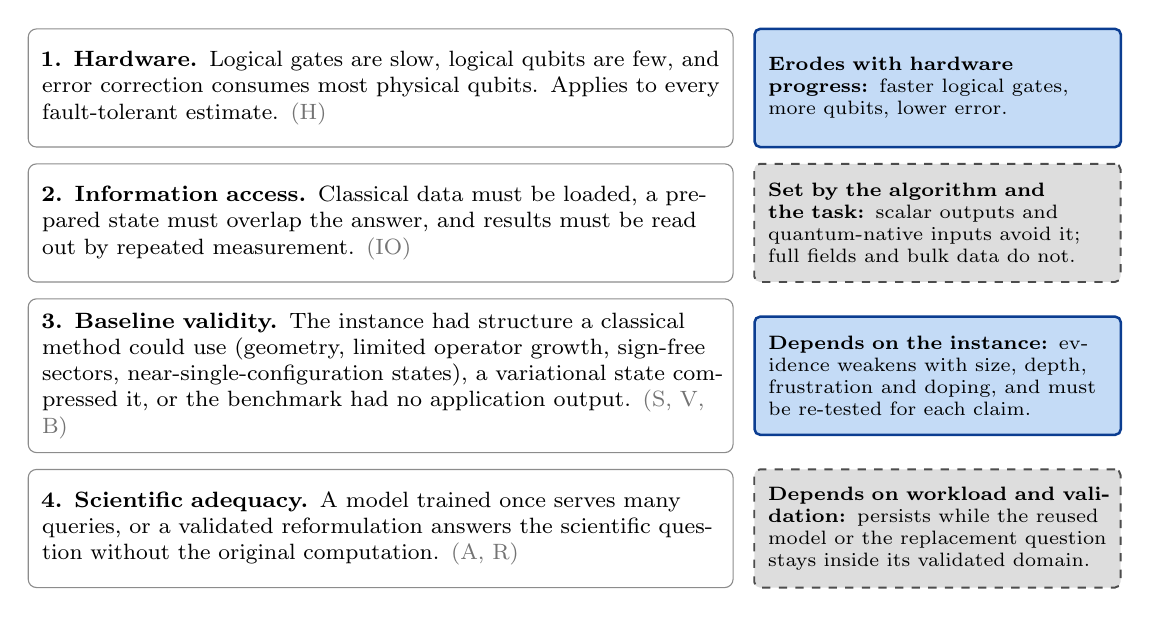
\begin{tikzpicture}[
  grp/.style={draw=black!45, rounded corners=3pt, align=left, inner sep=5pt, font=\footnotesize, text width=8.6cm, minimum height=1.5cm},
  tag/.style={rounded corners=2pt, align=left, font=\scriptsize, text width=4.3cm, inner sep=5pt, minimum height=1.5cm},
  node distance=0.2cm]
\node[grp] (h) {\textbf{1. Hardware.} Logical gates are slow, logical qubits are few, and error correction consumes most physical qubits. Applies to every fault-tolerant estimate. \textcolor{black!55}{(H)}};
\node[grp, below=of h] (io) {\textbf{2. Information access.} Classical data must be loaded, a prepared state must overlap the answer, and results must be read out by repeated measurement. \textcolor{black!55}{(IO)}};
\node[grp, below=of io] (s) {\textbf{3. Baseline validity.} The instance had structure a classical method could use (geometry, limited operator growth, sign-free sectors, near-single-configuration states), a variational state compressed it, or the benchmark had no application output. \textcolor{black!55}{(S, V, B)}};
\node[grp, below=of s] (a) {\textbf{4. Scientific adequacy.} A model trained once serves many queries, or a validated reformulation answers the scientific question without the original computation. \textcolor{black!55}{(A, R)}};
\node[tag, right=0.25cm of h, fill=qcFl!60, draw=qcQ, line width=0.9pt] {\textbf{Erodes with hardware progress:} faster logical gates, more qubits, lower error.};
\node[tag, right=0.25cm of io, fill=qcNl!70, draw=black!70, dashed, line width=0.7pt] {\textbf{Set by the algorithm and the task:} scalar outputs and quantum-native inputs avoid it; full fields and bulk data do not.};
\node[tag, right=0.25cm of s, fill=qcFl!60, draw=qcQ, line width=0.9pt] {\textbf{Depends on the instance:} evidence weakens with size, depth, frustration and doping, and must be re-tested for each claim.};
\node[tag, right=0.25cm of a, fill=qcNl!70, draw=black!70, dashed, line width=0.7pt] {\textbf{Depends on workload and validation:} persists while the reused model or the replacement question stays inside its validated domain.};
\end{tikzpicture}
\caption[Four explanations for classical capability]{Four groups of explanation for why a classical or AI method answers a problem proposed for a quantum computer, and how each responds to quantum progress. Right-hand boxes with a solid border: progress in hardware or a harder instance can remove the explanation. Right-hand boxes with a dashed border: the explanation persists under stated workload and adequacy conditions. Letters are the codes used in the appendix tables. An explanation that has not been exploited for an instance has not been shown to be absent, and several usually apply to one case.}
\label{fig:taxonomy}
\end{figure}

In the device claims we reviewed, the classical response rarely came from AI being clever where quantum computing is brute force. More often the instance was easier than the worst case its quantum algorithm was designed for, and a structured method found and used that slack. Fig.~\ref{fig:taxonomy} sorts the explanations into four groups.

\textbf{Hardware.} A logical quantum operation is many orders of magnitude slower than a classical one, so a quadratic speedup needs an enormous problem before it pays off~\cite{hoefler2023,babbush2021}. Section~\ref{sec:breakeven} gives the model. Structured speedups of higher degree are known exceptions~\cite{babbush2025}.

\textbf{Information access.} A quantum algorithm that is fast once its input is loaded and before its output is read can lose its advantage at either end~\cite{aaronson2015,hoefler2023}. Linear solvers are the clearest case (Section~\ref{sec:linear}). Phase estimation depends in the same way on the overlap between a prepared state and the state sought (Section~\ref{sec:qpe}).

\textbf{Baseline validity.} Three kinds of structure answered the device claims of Section~\ref{sec:devices}: tree-like correlations that belief propagation contracts efficiently~\cite{tindall2024}, limited growth of operators in the regime studied~\cite{begusic2024}, and boundary geometry that fixed the cost of contracting a circuit~\cite{manabe2026}. In chemistry, the hard part of one flagship model turned out to be ranking many states that are each close to a single configuration~\cite{zhai2026}, and Lee et al.\ find that features which make a state easy to prepare on a quantum computer also tend to make classical heuristics work~\cite{lee2023}. Some lattice instances have no sign problem for quantum Monte Carlo~\cite{hirsch1985}. Variational states, neural or not, are not limited by entanglement growth in the way matrix-product states are~\cite{mauron2025}. And some benchmarks have no application output at all. Where this evidence weakens depends on the method and the regime: doped and frustrated lattices, multireference active spaces where DMRG cost rises steeply~\cite{goings2022}, and long-time dynamics with high entanglement~\cite{bermejo2026}. A sign problem is a warning about one method, not a guarantee of quantum superiority.

\textbf{Scientific adequacy.} A model trained once can serve many queries, and a learned reformulation can answer the scientific question without the original computation (Section~\ref{sec:ai}). Both hold only inside a validated domain.

\subsection{The record behind the numbers}
Every number in a figure or a ratio comes from a ledger of eight linked tables (Appendix~\ref{app:ledger}). A value may enter a figure only if we read it at a table or section of a source whose version is identified by the document itself: an arXiv identifier with its version number, or a journal reference. Values known only from an abstract or at second hand stay in the tables, may be quoted in the text with that level stated, and are refused by the validation script if a figure cites them. For each headline comparison we record the task, output, accuracy and cost conditions; missing details are marked explicitly, and a completeness table shows how many remain (Appendix~\ref{app:ledger}). The same scrutiny is applied to both sides. A quantum record should state its state-preparation assumptions, its repetitions, the bias of any error mitigation and the domain in which that mitigation was tested. A learned-model record should state the shift between training and target domains, the cost and source of its labels, its uncertainty calibration and its dependence on seed and optimizer.

\subsection{The evidence in one table}
Table~\ref{tab:summary} condenses the map to twelve rows. The full list of \nEntries{} entries is in Appendix~\ref{app:entries}.

{\small
\setlength{\tabcolsep}{4pt}
\begin{longtable}{@{}L{3.0cm} L{4.7cm} L{4.1cm} L{4.1cm}@{}}
\caption{The evidence in brief, as of 11 November 2026. Identifiers refer to Appendix~\ref{app:entries} (entries) and Appendix~\ref{app:forward} (classes).}\label{tab:summary}\\
\toprule
Scientific task & Evidence obtained & What is unresolved & Next decisive test\\
\midrule\endfirsthead
\toprule
Scientific task & Evidence obtained & What is unresolved & Next decisive test\\
\midrule\endhead
\bottomrule\endfoot
Sampling benchmarks (E01, E02, E24--E26, E34--E36) & Four experiments answered at their validation statistic by tensor networks or a classical sampling algorithm and two challenged on it by mock-up samplers; the newest instances are unanswered & Efficient sampling of any full output distribution; later device generations & A classical response to the revised circuits, or fresh samples at stated fidelity\\
Kicked-Ising dynamics, 127 qubits (E03) & Reported observables reproduced in 12 days by tensor networks and Pauli propagation on a laptop & Larger and deeper circuits of the same family & A converged classical result at 100 spins and the depth of the related fault-tolerant estimate\\
Spin-glass quench dynamics on an annealer (E04) & Classical errors below the device in some regimes; other observables and lattices not reproduced & Three-dimensional lattices at long times; high-order correlations & Stable long-time variational or tensor-network dynamics at the claimed scales\\
Coherent dynamics on gate-model devices (E05--E07, E23) & Four claims with no converged classical method in the hardest regime tested; classical predictions disagree with each other in one & Whether the device results are accurate there; whether other classical methods converge & Validation across the hard regime with mitigation overhead costed; a converged classical reproduction\\
Approximate optimization (E18, E27) & Two scaling claims, each contested by a wider classical solver portfolio & Scaling on a defined instance family under one runtime convention & A separation from the full portfolio with matched accounting\\
Iron--sulfur clusters and embedded protein--ligand chemistry (E09, E28) & Hybrid workflows at scale with no advantage claimed; the circuit energy is classically computable for single-layer circuits & What the quantum samples add & An ablation that replaces quantum samples with classical ones\\
Ground states of 2D Hubbard and Heisenberg models (classes 6, 7) & Modelled quantum schedules of hours to a day against DMRG estimates on four CPU cores & The best classical cost; the half-filled Hubbard model is free of the sign problem & A Monte Carlo, neural-state or parallel DMRG time on the same lattice and tolerance\\
FeMoco and P450 energies (E10; classes 10, 11) & Classical energy of the 76-orbital model to about 1 kcal/mol by extrapolation; 2026 quantum estimates of 2.5 to 5.3 hours per accepted run on 1.2 to 2.7 million physical qubits & Overlap of the prepared state; repetitions; a spin gap needs two states; classical cost at matched confidence & A measured overlap and full protocol cost; a classical gap converged at a stated tolerance\\
Core-level X-ray absorption (class 9) & A quantum estimate that covers preparation, sampling and the full spectrum: about \xasHours{} hours at an assumed 1\,MHz logical clock & Initial-state quality; the error model; the clock; the best classical spectrum & A classical spectrum for the same cluster; validated preparation\\
Sparse linear systems, finite elements and fluid dynamics (E32, E33; class 38) & Limits to polynomial speedup for stated problems in fixed dimension; a partial estimate of $10^{21}$ to $10^{39}$ in qubits times T gates for the drag on a sphere; no practical advantage established & Conditional polynomial proposals for structured inputs and selected observables; high-dimensional and quantum-native linear problems & A complete estimate below a tuned classical solver at an industrial condition number; a classical spectral baseline for the compressed Navier--Stokes task\\
Materials and molecular screening (E12--E14) & AI+HPC screens validated by synthesis and measurement; a learned functional at chemical accuracy on main-group benchmarks & Transition-metal and multireference cases where labels are scarce & A decision-critical electronic-structure bottleneck shown to dominate the error budget\\
Neural wavefunctions for lattices, molecules and nuclei (E22, E29, E30) & Variational energies below DMRG on a frustrated lattice; nuclei to mass number 20 & Ansatz bias; cost at a fixed certified accuracy; no result on the instances of the quantum estimates & Neural-state results on those instances with convergence reported\\
\end{longtable}
}
% =====================================================================
\section{What device experiments show}
\label{sec:devices}

\pgfplotsset{timelineaxis/.style={ytick={1,...,16}, ymin=0.4, ymax=16.6, yticklabels={{Google Sycamore RCS, 53 q (2019)}, {Xanadu Borealis GBS (2022)}, {USTC Jiuzhang 3.0 GBS (2023)}, {IBM doped Clifford, 70 q (v1, 2026)}, {USTC Jiuzhang GBS, 100 modes (2020)}, {USTC Jiuzhang 2.0 GBS (2021)}, {IBM Eagle kicked Ising, 127 q (2023)}, {D-Wave annealing dynamics (v1, 2024)}, {D-Wave QAC optimization (v1, 2024)}, {Harvard Rydberg MIS, 289 atoms (2022)}, {Quantinuum H2 magnetism, 56 q (2025)}, {Google OTOC(2), 65 q (2025)}, {IBM--Algorithmiq OLE, 56 q (2025)}, {USTC ultracold atoms, 64 sites (v2, 2026)}, {IBM Heron Floquet, 74 q (v1, 2026)}, {IBM doped Clifford, 64 q (v2, 2026)}}}}

\begin{figure}[htbp]
\centering
\begin{tikzpicture}
\begin{axis}[
  xbar, width=0.56\textwidth, height=11.3cm,
  xmin=0, xmax=38, y dir=reverse, timelineaxis,
  yticklabel style={font=\footnotesize},
  xlabel={\footnotesize Months from first public claim (days / 30.44); open claims to 11 Nov 2026},
  xticklabel style={font=\footnotesize},
  bar width=7pt, bar shift=0pt,
  xmajorgrids, grid style={black!12},
  axis x line*=bottom, axis y line*=left, clip=false,
  legend style={font=\scriptsize, at={(0.5,1.02)}, anchor=south, draw=black!25, fill=white, legend columns=3}, legend cell align=left]
\addplot[fill=qcN, draw=black!75, line width=0.3pt, nodes near coords={\pgfmathprintnumber[fixed,precision=1]{\pgfplotspointmeta}\,mo, matched}, point meta=x, every node near coord/.append style={font=\scriptsize, anchor=west}] table[x=x,y=y] {figdata/timeline_validation.dat};
\addlegendentry{validation benchmark matched}
\addplot[fill=white, draw=black!75, line width=0.3pt, postaction={pattern=north east lines, pattern color=black!70}, nodes near coords={\pgfmathprintnumber[fixed,precision=1]{\pgfplotspointmeta}\,mo, challenged}, point meta=x, every node near coord/.append style={font=\scriptsize, anchor=west}] table[x=x,y=y] {figdata/timeline_challenged.dat};
\addlegendentry{validation statistic challenged}
\addplot[fill=black!85, draw=black!85, line width=0.3pt, nodes near coords={\pgfmathprintnumber[fixed,precision=1]{\pgfplotspointmeta}\,mo, reproduced}, point meta=x, every node near coord/.append style={font=\scriptsize, anchor=west}] table[x=x,y=y] {figdata/timeline_observables.dat};
\addlegendentry{observables reproduced}
\addplot[fill=qcNl, draw=black!75, line width=0.3pt, postaction={pattern=dots, pattern color=black!80}, nodes near coords={$\approx$\pgfmathprintnumber[fixed,precision=1]{\pgfplotspointmeta}\,mo, partly}, point meta=x, every node near coord/.append style={font=\scriptsize, anchor=west}] table[x=x,y=y] {figdata/timeline_partial.dat};
\addlegendentry{observables partly reproduced}
\addplot[fill=qcUl, draw=qcUd, line width=0.3pt, postaction={pattern=crosshatch, pattern color=qcU}, nodes near coords={\pgfmathprintnumber[fixed,precision=1]{\pgfplotspointmeta}\,mo, contested}, point meta=x, every node near coord/.append style={font=\scriptsize, anchor=west}] table[x=x,y=y] {figdata/timeline_contested.dat};
\addlegendentry{contested}
\addplot[fill=qcF, draw=qcQ, line width=0.3pt] table[x=x,y=y] {figdata/timeline_open.dat};
\addlegendentry{open (right-censored)}
\addplot[quiver={u=3.2,v=0}, -{Latex[length=2.2mm]}, qcF, line width=1.2pt, forget plot] table[x=x,y=y] {figdata/timeline_open.dat};
\addplot[only marks, mark=none, forget plot, nodes near coords={\textbf{$\ge$\pgfmathprintnumber[fixed,precision=1]{\pgfplotspointmeta}\,mo, open}}, point meta=x, every node near coord/.append style={font=\scriptsize, anchor=west, qcF, xshift=22pt}] table[x=x,y=y] {figdata/timeline_open.dat};
\end{axis}
\end{tikzpicture}
\caption[Time from quantum claim to classical response]{Time from first public claim to first classical response for the \nTimeline{} device claims that meet the eligibility rule: \emph{a claim that a quantum device performed a computation faster or at larger scale than the best stated classical method}. The kind of response (Section~\ref{sec:match}) is printed in words at the end of each bar and repeated in the fill: a plain mid-tone bar for a matched validation benchmark, diagonal hatching for a challenged validation statistic, a plain dark bar for reproduced observables, dots for a partial reproduction, cross-hatching for a contested response, and a bar ending in an arrow for an open claim; arrows mark claims still open on 11 November 2026, from which no rate is inferred. Each row is one instance and version. A short bar records a fast response to a specified test; an open bar records the absence of a qualifying response, not evidence of impossibility. For Jiuzhang~2.0 the bar is the 2021 challenge, and the 2023 match is described in the text. A response to the 70-qubit doped Clifford circuit does not stop the clock for its 64-qubit successor, and the ultracold-atom clock starts at the April 2026 version that first reported 64 sites. The operator-Loschmidt-echo row is plotted from 30 November 2025, a lower bound on its age. Later random-circuit generations and the newest boson-sampling generation are not entered. Dates and sources are in \texttt{entries.csv}.}
\label{fig:timeline}
\end{figure}

Fig.~\ref{fig:timeline} places \nTimeline{} device claims on a common clock. Of these, \wTLvalidation{} were answered by matching the statistic the experiment used to validate itself, \wTLchallenged{} were challenged on such a statistic by classical mock-up samplers, \wTLobservables{} by reproducing its reported observables and \wTLpartial{} in part; \wTLcontested{} are contested and \wTLopen{} have no published classical match as of 11 November 2026. The answered claims took between 12 days and 24 months. The open ones are between \eld{E25} and \eld{E05} days old. The figure is a record of what happened to these claims. It is not a survival curve, and the open bars predict nothing. Each case below is described by the same five questions: what scientific output is at stake, what each side computed, what kind of evidence that is, what remains unresolved, and what result would settle it.

\subsection{Sampling benchmarks}
\textbf{Question.} Can a device draw samples from a probability distribution that no classical computer can sample at comparable quality? These experiments test capability and have no application output.

\textbf{What was done.} Google's Sycamore sampled random 53-qubit circuits in 2019~\cite{arute2019}, and USTC's Jiuzhang sampled photons from a Gaussian boson network from 2020~\cite{zhong2020}; larger random-circuit experiments followed at Google, USTC and Quantinuum. In July 2026 IBM sampled a 70-qubit circuit of Clifford gates doped with 468 T gates, using error-detecting spacetime codes to certify fidelity~\cite{martiel2026}. USTC sampled a driven Bose--Hubbard system of up to 64 lattice sites and 20 atoms in a quantum gas microscope and reported a sampling rate three orders of magnitude above a supercomputer~\cite{zheng2026}; that claim dates from the April 2026 version of the paper, whose 2022 first posting described a 32-site chain as comparable to the fastest supercomputer.

\textbf{Classical side and evidence.} Tensor-network contraction produced Sycamore-sized samples at comparable XEB values after 24 months~\cite{pan2022}. The boson-sampling experiments are recorded one by one. Mock-up samplers built from low-order marginals came closer than the experiment to the ideal marginals, in total variation distance, for the 2020 100-mode data and for Jiuzhang~2.0, \eld{E34} and \eld{E02} days after those claims~\cite{villalonga2021}. A classically sampleable optical state was not ruled out as an explanation of the 2020 data, while the same tests favoured the quantum model for Jiuzhang~2.0~\cite{martinez2023}. These studies challenge particular validation statistics; they do not sample from the complete ideal distribution. A tensor-network algorithm later outperformed Jiuzhang~2.0~\cite{zhong2021}, Jiuzhang~3.0~\cite{deng2023} and Borealis~\cite{madsen2022} on the statistics used to validate them~\cite{oh2024}, \eld{E36} days after Jiuzhang~3.0 and \eld{E35} days after Borealis. A polynomial-time classical sampler now exists for the distribution used by graph applications of boson sampling; that is a result about that distribution and not about these experiments~\cite{anand2026}. For IBM's 70-qubit circuit, Manabe, Gu and Pan computed the amplitudes of all 2{,}051 published batches of bitstrings in \dcMin{} minutes on 256 GPUs, \eld{E24} days after the claim; the largest intermediate tensor was 256 times smaller than the experiment's authors had estimated~\cite{manabe2026}. The four matches are to a validation benchmark and the two challenges to a diagnostic of one, and each date in Fig.~\ref{fig:timeline} is that of the first response at the validation statistic, which need not be the first cost-competitive reproduction. Amplitudes of published outputs are not fresh samples, and none of these responses shows that a full output distribution can be sampled efficiently.

\textbf{Unresolved.} IBM replaced the circuit in September 2026 with a 64-qubit version of depth 73 with 314 T gates on a ring of qubits; its text states that periodic boundaries remove the contraction path the classical response used~\cite{martiel2026}. We found no classical response to that instance, to the ultracold-atom experiment, to later random-circuit experiments or to the newest boson-sampling generation. Hangleiter concludes that advantage holds for finite-fidelity random-circuit sampling at the level of experimental physics~\cite{hangleiter2026}. The ultracold-atom experiment is validated by Bayesian tests against alternative hypotheses, which do not certify closeness to the ideal distribution.

\textbf{Next test.} A classical response to either revised instance, or sampling at a stated fidelity. An unanswered instance is not an established hardness result, and the three doped Clifford records (original, response, revision) should not be merged into ``refuted'' or ``unrefuted''.

\subsection{Dynamics claims that were answered}
\textbf{Kicked Ising model on 127 qubits (E03).} IBM's Eagle processor ran up to 20 steps of a periodically kicked transverse-field Ising model on its heavy-hexagon lattice and estimated magnetizations by zero-noise extrapolation~\cite{kim2023}. The output is a set of local expectation values. Within 12 days, belief-propagation tensor networks matched to the lattice geometry gave results more accurate than the mitigated data~\cite{tindall2024,aps2024}, and sparse Pauli dynamics reproduced them on one laptop core~\cite{begusic2023,begusic2024}; a dissipative mean-field picture accounts for the experiment's resilience to noise~\cite{dallatorre}. The classical calculations targeted the ideal circuit, so this is reproduction of observables. The explanation is structure: correlations on this lattice are close to tree-like, where belief propagation is exact, and operators grow slowly in the parameter regime studied. A related fault-tolerant target, 100 spins for ten Trotter steps, has a published estimate of 230 logical qubits and $2.4\times10^6$ T gates per execution with repetitions uncosted~\cite{beverland2022}; a converged classical result at that size and depth would answer it.

\textbf{Spin-glass quenches on an annealer (E04).} D-Wave's Advantage2 annealer followed the quench dynamics of Ising spin glasses on two-, three- and infinite-dimensional lattices and reported agreement with the Schr\"odinger equation beyond the reach of the classical methods it tested~\cite{king2025}. A year later, lattice-matched tensor networks~\cite{tindall2025} and time-dependent variational Monte Carlo with Jastrow--Feenberg wavefunctions on up to 128 spins~\cite{mauron2025} reached lower errors than the device in some regimes. Full-state and fourth-order observables were not reproduced, and coverage by lattice, quench time and observable is partial~\cite{kingreply}. The claim is partly answered and contested. Stable long-time variational dynamics in three dimensions at the claimed scales would close it from the classical side; observables beyond classical coverage at matched error would close it from the quantum side.

\subsection{Dynamics claims that stand}
Four claims have no published classical reproduction in their hardest regime. In each, the status is scoped to the methods tested and the criterion stated. It is not a hardness theorem, and disagreement among classical methods shows classical difficulty, not correctness of the quantum result.

\textbf{Out-of-time-order correlators (E06).} An out-of-time-order correlator measures how a local disturbance spreads through a quantum system. Google measured a second-order correlator on 65 qubits of its Willow processor~\cite{google2025otoc}. The primary paper reports 2.1 hours of data collection per circuit and estimates about 3.2 years for tensor-network simulation of one circuit on the Frontier supercomputer, a reported ratio of roughly 13{,}000~\cite{google2025otoc,googleblog2025}. This compares a measured acquisition time with a modelled classical cost. At 40 qubits the measured correlator is checked against exact simulation; at 65 qubits its accuracy is estimated from an empirical error model, and the comparison has not been independently reproduced. We list the two figures and do not plot a ratio. A test by Google co-authors finds the circuits largely incompressible for tensor-network evolution in the Schr\"odinger picture~\cite{bermejo2026}. Open for \eld{E06} days.

\textbf{Floquet magnets on two platforms (E05, E23).} Quantinuum's H2 trapped-ion processor simulated a periodically driven Ising model on a $7\times8$ lattice of 56 qubits; tensor-network, neural-network and operator-truncation methods were tested and none converged in the hardest regime~\cite{haghshenas2025}. Open for \eld{E05} days. IBM's Heron processor, with the QESEM error-mitigation software, measured magnetization on heavy-hexagon ladders of up to 74 qubits and resolved long-lived oscillations~\cite{leviatan2026}. The authors report that tensor networks do not converge and that sparse Pauli-path results depend on truncation, including runs on GPUs and on Fugaku. Their validation has several layers: an unbiased and an extrapolated estimator agree over the time window they share; the deepest and largest results rely on extrapolation; trapped-ion hardware corroborates selected cycles; and the conclusion that oscillations persist in the thermodynamic limit is a finite-size extrapolation. Three questions are therefore separate: whether the trajectory was measured reliably in the tested domain, whether a tested classical method converged there, and whether the extrapolation holds. Open for \eld{E23} days. This is a different task from the 2023 Eagle experiment, and the earlier classical response does not answer it.

\textbf{Operator Loschmidt echo (E07).} IBM and Algorithmiq measured an echo observable on 56 qubits~\cite{barron2026,ibmalgo2026}. Three classical groups produced predictions that disagree with one another. The quantum evidence has two parts of different strength: a heuristic rescaling argument supported by consistency tests across five noise settings on two processors, and a conditional route to error bounds that relies on noise characterization.

\textbf{What would settle these.} From the classical side, a converged reproduction of the stated observable at the stated depth and precision. From the quantum side, validation across the hard regime with the measurement overhead of error mitigation included. Error mitigation estimates a less noisy result from additional noisy runs and a noise model; its bias and its cost both matter. No fault-tolerant compilation exists for any of these observables.

\subsection{Optimization claims that are contested}
\textbf{Annealing with error suppression (E18).} D-Wave hardware with quantum annealing correction, on more than 1{,}300 error-suppressed encoded variables, showed better scaling of time-to-solution than parallel tempering with cluster moves for approximate solutions within 1\% of optimal~\cite{munoz2025,dwave_qac}. A follow-up with the simulated bifurcation machine, a classical dynamical solver, finds comparable or better scaling and concludes that current annealers are unlikely to show a clear advantage on these problem families under its accounting~\cite{pawlowski2026}. The two sides use different runtime conventions and solver portfolios, and that difference is the substance of the dispute.

\textbf{Maximum independent set on Rydberg arrays (E27).} A Harvard experiment on up to 289 atoms reported a superlinear speedup over simulated annealing on the hardest graphs~\cite{ebadi2022}. Andrist et al.\ then solved quasi-planar instances with thousands of nodes to optimality within minutes on commodity hardware and found a relaxed annealer competitive with the quantum algorithm on those instances; the same authors propose harder instances~\cite{andrist2023}.

Both cases teach the lesson of the lattice models in Section~\ref{sec:lattice}: a wider classical portfolio changes an advantage claim. The test that would settle either is a scaling separation from the full portfolio on a defined instance family, with one runtime convention, a stated quality gap and wall time reported. Other proposals fit neither search nor annealing, such as quantum-proposed moves inside a classical Markov chain~\cite{layden2023,orfi2024,marshall2026,hsieh2026}; these need time per statistically independent sample as their metric (class 37).

\subsection{Hybrid workflows that claim no advantage}
\textbf{Iron--sulfur clusters and protein--ligand complexes (E09, E28).} In sample-based quantum diagonalization, a quantum processor samples electronic configurations and a supercomputer diagonalizes the Hamiltonian in the subspace they span. Experiments on IBM Heron processors with Fugaku reached a [4Fe-4S] cluster with 77 qubits, and a closed-loop run used all 152{,}064 Fugaku nodes~\cite{shirakawa2025}. A 2026 study embeds such fragment solvers in two protein--ligand complexes of about 12{,}000 atoms, using up to 94 qubits, \merzCircuits{} circuits and \merzQpu{} processor-hours~\cite{merz2026}. Neither claims an advantage, and both demonstrate integration at scale. Three classical results bound what the quantum part contributes. The energy of the single-layer circuits used can be evaluated classically in polynomial time, reproducing the 77-qubit energy on a laptop in under a minute~\cite{belagali2026}. Sampling from an ideal ground state yields less compact expansions than classical selection: 50{,}551 determinants against 4{,}260 at a 0.1\,Ha error for [2Fe-2S]~\cite{reinholdt2025}. And GPU-accelerated DMRG reaches the [4Fe-4S] active-space size in \feDmrgH{} hours on one node~\cite{legeza2026}, although we have not confirmed that its Hamiltonian is identical to the experiment's. In the protein--ligand study, fragment energies lie 0.10 to 2.3\,mHa above DMRG and classical selected configuration interaction is more accurate on one fragment. Agreement of a binding energy, the error of the fragment solver and the contribution of the quantum sampler are three separate tests; the study reports the second, presents a binding prediction and does not test the third. Further classical results on these subspace methods are reviewed in~\cite{bonilla2026}. What is missing in both is an ablation: the same selection, recovery and diagonalization pipeline fed with classical samples in place of quantum ones.

\textbf{Protein fragments and drug candidates (E15, E16).} Variational quantum folding of short peptides on a lattice produced a structure 1.781\,\AA{} from experiment where the exact optimum of the same lattice model gave 1.879\,\AA~\cite{robert2021,doga2024}. That is not a computational advantage: the device did not optimize the model better than an exact solver, and the model's optimum need not be the most accurate structure. A 2026 study reports better fragment structures than AlphaFold3 under identical post-processing~\cite{zhang2026}; whether classical samplers under the same selection rule match it is untested. A quantum generative prior for KRAS inhibitors gave a modest benchmark gain and two promising synthesized molecules, and its authors state that this does not show superiority over classical priors~\cite{kras2025,uoft2025}. In all three, the quantum contribution has not been isolated.

\subsection{What the device record shows}
Three observations follow. First, every successful response in this set used structured numerical or classical variational methods. No neural network was needed, which is a statement about these responses and not about neural methods (Section~\ref{sec:ai}). Second, a response answers one instance. The doped Clifford and ultracold-atom cases show how a revised experiment restarts the clock, and the Floquet cases show that an answer on one lattice and depth does not carry to another. Third, the standing claims are all coherent dynamics or sampling at depths where known classical representations fail to converge, and each rests on a validation step whose accuracy in that regime is what is in question. The step differs by case: error mitigation or an error model calibrated at smaller sizes for the digital dynamics experiments, error detection with post-selection for the doped Clifford circuits, and statistical tests against alternative hypotheses for the analog sampler. An analog experiment adds a different caution: a Rydberg-atom spin liquid was later simulated variationally at 288 atoms, and the simulated state shows topological order but lacks the entanglement-entropy signature of the resonating-valence-bond state usually associated with it~\cite{semeghini2021,mauron2025tee}; the entropy itself was not measured, although randomized measurements could estimate it~\cite{brydges2019}, so classical simulation there complements the experiment and does not replace it.
% =====================================================================
\section{Where fault-tolerant estimates stand}
\label{sec:ft}

\subsection{How to read a resource estimate}
A fault-tolerant quantum computer combines many \emph{physical} qubits into fewer \emph{logical} qubits that are protected against errors. A resource estimate for an algorithm reports some of the following, and the differences between them are large.
\begin{itemize}
\item \textbf{Logical width}: the logical qubits the algorithm occupies. Sources count it differently. Some give the minimum workspace; others include routing space or memory, or exclude the factories described next.
\item \textbf{Non-Clifford gate count}: the number of T gates, or of Toffoli (CCZ) gates. These are the expensive operations. Each consumes a specially prepared ``magic'' state produced by a \emph{factory}, an error-corrected subroutine that can occupy most of the machine. T and Toffoli counts are different units and are not interchangeable here.
\item \textbf{Physical qubits and runtime}: derived from a code, a physical error rate, a code-cycle time and a classical reaction time. Runtime may be quoted for one shot or as an expected value that includes repeats after detected failure.
\item \textbf{What is left out}: commonly the preparation of the initial state, the number of repetitions needed for a reliable answer, and every calculation after the first.
\end{itemize}
Fig.~\ref{fig:dumbbell} shows the five cases in which a modelled quantum time and an estimated classical time exist for one model and tolerance. None of the plotted values is a measured runtime, and the cases below explain what each one covers. The full list of resource records is Table~\ref{tab:worked} in Appendix~\ref{app:models}.

\begin{figure}[htbp]
\centering
\begin{tikzpicture}
\begin{axis}[
  xmode=log, width=0.56\textwidth, height=8.0cm,
  xmin=0.2, xmax=3e7, ymin=0.4, ymax=5.6, y dir=reverse,
  ytick={1,...,5},
  yticklabels={{Fermi--Hubbard 6$\times$6, half filling\\{\scriptsize\color{black!60} model schedule vs 4-core DMRG estimate}}, {Fermi--Hubbard 10$\times$10, half filling\\{\scriptsize\color{black!60} model schedule vs 4-core DMRG estimate}}, {$J_1$--$J_2$ Heisenberg 10$\times$10\\{\scriptsize\color{black!60} model schedule vs 4-core DMRG estimate}}, {FeMoco, 76 orbitals, 1 kcal/mol\\{\scriptsize\color{black!60} model expectation vs idealized estimate, not run}}, {P450 compound I, 58 orbitals\\{\scriptsize\color{black!60} model expectation vs 2022 source estimate}}},
  yticklabel style={font=\footnotesize, align=right},
  xlabel={\footnotesize Published time estimate (hours, log scale)},
  xticklabel style={font=\footnotesize},
  xmajorgrids, grid style={black!10}, axis y line*=left, axis x line*=bottom, clip=false,
  legend style={font=\scriptsize, at={(0.5,-0.15)}, anchor=north, draw=black!25, fill=white, legend columns=2}, legend cell align=left]
\draw[black!20, line width=1.4pt] (axis cs:3.4167,1) -- (axis cs:61.111,1);
\draw[black!20, line width=1.4pt] (axis cs:29.167,2) -- (axis cs:1.9722e6,2);
\draw[black!20, line width=1.4pt] (axis cs:15.667,3) -- (axis cs:21.944,3);
\draw[black!20, line width=1.4pt] (axis cs:1.11,5) -- (axis cs:720,5);
\draw[qcU!60, line width=1.4pt] (axis cs:5.26,4) -- (axis cs:42.08,4);

\addplot[only marks, mark=o, mark size=3pt, color=qcF, line width=1pt] table[x=x,y=y] {figdata/dumbbell_q_est.dat};
\addlegendentry{quantum, modelled schedule}
\addplot[only marks, mark=triangle, mark size=3.2pt, color=qcF, line width=0.9pt] table[x=x,y=y] {figdata/dumbbell_q_par.dat};
\addlegendentry{quantum, alternative schedule}
\addplot[only marks, mark=diamond, mark size=3.4pt, color=qcU, line width=1pt] table[x=x,y=y] {figdata/dumbbell_q_scen.dat};
\addlegendentry{quantum, repetition scenario (ours)}
\addplot[only marks, mark=square, mark size=2.8pt, color=black!65, line width=1pt] table[x=x,y=y] {figdata/dumbbell_c_est.dat};
\addlegendentry{classical, estimate}
% generated by ledger/make_figdata.py
\node[font=\scriptsize, inner sep=5pt, anchor=south] at (axis cs:61.1111,1) {61\,h};
\node[font=\scriptsize, inner sep=5pt, anchor=south] at (axis cs:1.97222e6,2) {$\sim$225\,y};
\node[font=\scriptsize, inner sep=5pt, anchor=south] at (axis cs:21.9444,3) {22\,h};
\node[font=\scriptsize, inner sep=5pt, anchor=north] at (axis cs:5.26,4) {5.3\,h};
\node[font=\scriptsize, inner sep=5pt, anchor=south] at (axis cs:22.9,4) {22.9\,h};
\node[font=\scriptsize, inner sep=5pt, anchor=north] at (axis cs:73.0556,5) {2022: 25--73\,h};
\node[font=\scriptsize, inner sep=5pt, anchor=south] at (axis cs:1.88,5) {2026: 1.1--1.9\,h};
\node[font=\scriptsize, inner sep=5pt, anchor=south] at (axis cs:720,5) {$\sim$1 month};

\node[font=\scriptsize, anchor=west, qcUd] at (axis cs:60,4.02) {\repAttempts{} or \repAttemptsSplit{} accepted runs: \repHours, \repHoursSplit\,h};
\end{axis}
\end{tikzpicture}
\caption[Modelled quantum and estimated classical times]{Modelled quantum times and estimated classical times for five cases in which both sides publish a value for one model and tolerance. No point is a measured runtime, and the type of each value is printed under its row. \emph{Lattice models:} circles are the single-factory phase-estimation schedules of the source's Table~S12 and triangles its 16-factory schedules, which use \parQubitLo--\parQubitHi{} times the physical qubits; squares are the source's DMRG estimates on four cores of one CPU for a variational state within 0.01 of the extrapolated energy~\cite{yoshioka2024}. \emph{FeMoco:} circle and triangle are the minimum-volume and fastest tabulated rows of the 2026 dense-code compilation~\cite{low2026dense}, each an expected duration that already includes repeats after detected logical failure; diamonds are our scenario for \repAttempts{} or \repAttemptsSplit{} accepted executions at a hypothetical hit probability of 0.5 (Section~\ref{sec:qpe}); the square is an idealized conversion for a DMRG calculation that was not performed~\cite{zhai2026}. \emph{P450:} circles are the 2022 estimates at physical error rates $10^{-3}$ and $10^{-5}$~\cite{goings2022}, triangles the 2026 rows~\cite{low2026dense}, and the square the 2022 source's own classical estimate. A connector shows that two values refer to one model. It implies no ranking where the two sides differ in confidence semantics or machine assumptions. Generated from the ledger.}
\label{fig:dumbbell}
\end{figure}

\subsection{Lattice models of correlated electrons}
\label{sec:lattice}
\textbf{Question.} The Fermi--Hubbard model, electrons hopping on a lattice with on-site repulsion $U$, and the frustrated $J_1$--$J_2$ Heisenberg spin model are the standard minimal models of correlated materials. The output considered here is a ground-state energy to a total-energy accuracy of 0.01 in the model's units.

\textbf{What was done.} Yoshioka et al.\ estimate the cost of quantum phase estimation in the surface code at a physical error rate of $10^{-3}$ and compare it with DMRG~\cite{yoshioka2024}. For the half-filled Hubbard model at $U/t=4$ on a $10\times10$ cylinder, the modelled schedule with one magic-state factory takes $1.05\times10^5$\,s (\hubTenQh{} hours) on $8.9\times10^5$ physical qubits; with sixteen factories it takes $1.46\times10^4$\,s on $5.4\times10^6$. For the Heisenberg model at $J_2/J_1=0.5$ on the same lattice the two schedules take $5.64\times10^4$\,s and $4.32\times10^3$\,s. The classical figures are the source's estimates of the DMRG time needed to produce a variational state within 0.01 of the extrapolated energy: $7.1\times10^9$\,s for the Hubbard case and $7.9\times10^4$\,s for the Heisenberg case (Fig.~\ref{fig:hubbard}).

\begin{figure}[htbp]
\centering
\begin{tikzpicture}
\begin{axis}[
  xmode=log, ymode=log, width=0.68\textwidth, height=6.6cm,
  xmin=12, xmax=130, ymax=3e10,
  xtick={16,32,36,64,100}, xticklabels={16,32,36,64,100},
  xlabel={\footnotesize Lattice sites (4$\times$4, 4$\times$8, 6$\times$6, 4$\times$16 and 8$\times$8, 10$\times$10)},
  ylabel={\footnotesize Estimated time to $\Delta E=0.01$ (s)}, ymin=1, clip=false,
  ticklabel style={font=\footnotesize}, grid=major, grid style={black!10},
  legend style={font=\scriptsize, at={(0.02,0.98)}, anchor=north west, draw=black!25, fill=white}, legend cell align=left]
\addplot[black!55, mark=square*, line width=0.9pt, mark size=2.2pt, dashed, mark options={solid}] table[x=x,y=y] {figdata/hubbard_U1.dat};
\addlegendentry{DMRG, square, $U/t=1$}
\addplot[qcF, mark=*, line width=1.2pt, mark size=2.4pt] table[x=x,y=y] {figdata/hubbard_U4.dat};
\addlegendentry{DMRG, square, $U/t=4$}
\addplot[qcU, mark=triangle*, line width=1.0pt, mark size=2.8pt, dashdotted, mark options={solid}] table[x=x,y=y] {figdata/hubbard_U8.dat};
\addlegendentry{DMRG, square, $U/t=8$}
\addplot[only marks, mark=o, mark size=2.6pt, qcF, line width=0.8pt] table[x=x,y=y] {figdata/hubbard_strip_U4.dat};
\addlegendentry{strips $4\times8$, $4\times16$ (hollow, same shapes)}
\addplot[only marks, mark=square, mark size=2.2pt, black!55, line width=0.8pt, forget plot] table[x=x,y=y] {figdata/hubbard_strip_U1.dat};
\addplot[only marks, mark=triangle, mark size=2.8pt, qcU, line width=0.8pt, forget plot] table[x=x,y=y] {figdata/hubbard_strip_U8.dat};
\addplot[only marks, mark=diamond*, mark size=3.6pt, qcQ] table[x=x,y=y] {figdata/hubbard_qpe_s.dat};
\addlegendentry{QPE, 1 factory (modelled)}
\addplot[only marks, mark=diamond, mark size=3.6pt, qcQ, line width=0.9pt] table[x=x,y=y] {figdata/hubbard_qpe_p.dat};
\addlegendentry{QPE, 16 factories (modelled)}
\end{axis}
\end{tikzpicture}
\caption[Half-filled Hubbard model: classical estimate and quantum model]{Half-filled two-dimensional Fermi--Hubbard model on cylinders. Filled symbols joined by lines (squares and a dashed line for $U/t=1$, circles and a solid line for $U/t=4$, triangles and a dash-dotted line for $U/t=8$): the source's estimated DMRG time, on four cores of one CPU, to a variational state within 0.01 of the extrapolated total energy, for square lattices (its Table~S2). Hollow symbols: narrow strips, which are far cheaper at equal site count and are not joined to the squares. Diamonds, filled and hollow: the source's modelled phase-estimation schedules at $U/t=4$ with one and with sixteen magic-state factories (its Table~S12)~\cite{yoshioka2024}. This instance has no sign problem for determinant and auxiliary-field quantum Monte Carlo~\cite{hirsch1985}; no Monte Carlo cost is shown because none has been compiled at this tolerance. Generated from the ledger.}
\label{fig:hubbard}
\end{figure}

\textbf{Evidence.} Both sides are models. Against this baseline the single-factory quantum schedule is faster by a factor of \ratioHubTen{} for the Hubbard lattice and \ratioHeis{} for the Heisenberg lattice. Three properties of the baseline limit what those ratios mean.
\begin{itemize}
\item \emph{Machine.} The DMRG times are for four cores of one CPU. The Hubbard figure is \hubTenCoreH{} core-hours, about three times the classical FeMoco campaign of Section~\ref{sec:chem} and the allocation equivalent of roughly \hubTenFugakuH{} hour of all Fugaku cores. That equivalence is a statement of budget and not a runtime, since DMRG does not parallelize ideally; the source itself expects about a tenfold gain from GPUs or several nodes, and GPU implementations now reach bond dimensions above $10^4$ on one node~\cite{legeza2026}.
\item \emph{Criterion.} The classical time is for a variational \emph{state} of the target accuracy. Phase estimation returns an energy, and the source notes that estimating the energy alone by extrapolation is much faster.
\item \emph{Method.} At half filling with nearest-neighbour hopping on a bipartite lattice, the Hubbard model has no sign problem for determinant and auxiliary-field quantum Monte Carlo~\cite{hirsch1985,leblanc2015}. The sign problem is the statistical cancellation that makes Monte Carlo expensive for most fermion problems; here it is absent. No Monte Carlo time-to-solution has been compiled at this tolerance, so the best classical baseline for this instance is unknown. For the Heisenberg benchmark on a periodic cluster, a transformer neural quantum state reaches a total energy 0.21 below a DMRG value at bond dimension 8{,}192~\cite{rende2024}. That is another geometry, but it shows that the cited DMRG calculation is not the best variational energy in that tabulated benchmark.
\end{itemize}

\textbf{Unresolved.} A measured classical speedup above \thrHeis{} over the four-core estimate would reverse the single-factory Heisenberg comparison, and one above \thrHeisPar{} would reverse the sixteen-factory comparison; neither has been measured. The Heisenberg case is therefore a small modelled margin whose sign depends on implementation and preparation assumptions. The Hubbard margin is large against DMRG and untested against Monte Carlo. On the quantum side, adiabatic state preparation is assumed to be cheap on the basis of fits up to 48 qubits. Doping, frustration or longer-range hopping restore the sign problem and define separate candidates, for which neural, tensor-network and embedding methods are the classical side (class 36). A recent experiment measured pairing correlations in a doped Hubbard model on trapped-ion hardware~\cite{granet2025}; pairing is a different observable from the ground-state energy.

\textbf{Next test.} A Monte Carlo, neural-state or parallel DMRG energy on the same cylinder at the same tolerance with a measured time; and a quantum estimate that includes preparation.

\subsection{Transition-metal chemistry: FeMoco and P450}
\label{sec:chem}

\textbf{Question.} FeMoco is the iron--molybdenum cofactor at which the enzyme nitrogenase reduces nitrogen, and cytochrome P450 is a family of enzymes that metabolize drugs. Their reactivity depends on the energies of closely spaced electronic states. Calculations treat an \emph{active space}: a chosen set of electrons and orbitals handled exactly, here 76 orbitals for FeMoco and 58 for the P450 intermediate compound~I. An active-space energy is not the chemistry of the enzyme. The usual target is \emph{chemical accuracy}, about 1\,kcal/mol or 1.6\,mHa.

\textbf{Quantum estimates.} Quantum phase estimation extracts an energy from a prepared state. Its cost for these models has fallen steadily. Tensor hypercontraction (2021) needs 2{,}196 logical qubits and $3.2\times10^{10}$ Toffoli gates for the 76-orbital FeMoco model; the frequently quoted four million physical qubits and four days belong to the smaller 54-orbital model, at 2{,}142 logical qubits and $5.3\times10^9$ Toffoli gates~\cite{lee2021thc}. A 2026 compilation into a dense surface-code layout tabulates a frontier of physical qubits against runtime for both molecules (Fig.~\ref{fig:dc76})~\cite{low2026dense}. For FeMoco it gives \femoT{} expected hours at \femoSevMinvolQ{} million physical qubits with \femoTofMinvol{} Toffoli gates (the row of minimum space--time volume), and \femoFastT{} hours at \femoSevFastQ{} million with \femoTofFast{} (the fastest row tabulated). For P450 it gives \pfMinvolH{} hours at 1.03 million and \pfFastH{} hours at 2.18 million, against 73 hours on 4.6 million in the 2022 estimate for the same model~\cite{goings2022}: about \pfSpeed{} times less time on \pfQubits{} times fewer qubits at the same error rate.

\begin{figure}[htbp]
\centering
\begin{tikzpicture}
\begin{groupplot}[group style={group size=2 by 1, horizontal sep=1.9cm}, width=0.47\textwidth, height=6.0cm, ticklabel style={font=\footnotesize}, label style={font=\footnotesize}, title style={font=\footnotesize}, xmode=log, ymode=log, xmin=5e4, xmax=8e6, grid=major, grid style={black!10}, xlabel={Physical qubits}, legend style={font=\scriptsize, draw=black!25, fill=white}, legend cell align=left]
\nextgroupplot[ymin=1, ymax=1e5, ylabel={Expected accepted runtime (hours)}, title={FeMoco, 76 orbitals}, legend pos=north east]
\addplot[qcF, mark=*, mark size=2.6pt, line width=0.6pt, densely dotted, mark options={solid}] table[x=x,y=y] {figdata/femoco76_dense.dat};
\addlegendentry{dense code, 2026}
\nextgroupplot[ymin=0.5, ymax=1e5, title={P450 Cpd I, model X (58 orbitals)}, legend pos=north east]
\addplot[qcF, mark=*, mark size=2.6pt, line width=0.6pt, densely dotted, mark options={solid}] table[x=x,y=y] {figdata/p450dc_dense.dat};
\addlegendentry{dense code, 2026}
\addplot[only marks, mark=square*, mark size=2.6pt, black!55] table[x=x,y=y] {figdata/p450dc_prior.dat};
\addlegendentry{THC, 2022}
\end{groupplot}
\end{tikzpicture}
\caption[FeMoco and P450: selected rows of the 2026 quantum cost frontier]{Each curve trades physical qubits against modelled time for one energy calculation; state preparation and the reliability of a useful answer are separate. Selected rows of the space--time frontier for phase estimation on the 76-orbital FeMoco model and the 58-orbital P450 model~\cite{low2026dense}. The vertical axis is the source's expected runtime. Dotted lines are guides to the eye between selected rows. Circles: rows of the 2026 dense-code compilation. Squares: the 2022 estimates for the same P450 model~\cite{goings2022}. Row selection and assumptions are in Appendix~\ref{app:models}. Generated from \texttt{resources.csv}.}
\label{fig:dc76}
\end{figure}

Two features of these numbers matter for any comparison. First, each runtime is an \emph{expected} value: the source divides the one-shot runtime by one minus the probability of a detected logical failure. For the FeMoco minimum-volume row that is \femoShot{} hours per shot at a failure probability of \femoPfail. Toward the low-qubit end failure dominates: at \femoSevLowQ{} physical qubits a 529-hour shot fails with probability \femoLowPfail{} and the expected time is 716 hours. Second, a successful shot is not yet a useful answer. Phase estimation returns the ground-state energy only with a probability set by how much the prepared state overlaps the ground state, so several accepted executions are needed, and no overlap has been measured for these models. Section~\ref{sec:qpe} works through the consequence: at a hypothetical hit probability of 0.5, \repAttempts{} or \repAttemptsSplit{} accepted executions, depending on how the failure budget is divided, or \repHours{} to \repHoursSplit{} expected hours.

\textbf{Classical results.} Zhai et al.\ computed the ground-state energy of the 76-orbital FeMoco model with unrestricted DMRG at bond dimensions up to 18{,}000 and high-order coupled cluster, starting from 78{,}750 broken-symmetry guesses~\cite{zhai2026}. The result agrees between methods to $\pm0.31$\,kcal/mol and has a conservative range of $\pm1.25$\,kcal/mol. Both rest on extrapolation, so this is approximately chemical accuracy with an empirical uncertainty, not a certified interval. The insight behind it is structural: the hard part is ranking many candidate states that are each close to a single configuration. The source's cost statements are three separate records.
\begin{itemize}
\item \emph{Measured:} the DMRG campaign took 2{,}768{,}994 core-hours, of which one sweep at bond dimension 18{,}000 took 317{,}440.
\item \emph{Modelled, not performed:} two variational sweeps at a bond dimension near 393{,}000 would take \femoClassCoreH{} core-hours by the fitted cost law, which the source converts to \femoClassIdeal{} hours on an exascale machine at ideal efficiency. The same conversion gives \femoUcc{} seconds for a coupled-cluster estimate. The source describes these as upper bounds that omit practical implementation factors.
\item \emph{Not costed:} constructing and ranking the candidate states.
\end{itemize}
For the P450 model the 2022 source measured DMRG on a smaller model and \emph{estimated} 36{,}564 CPU-hours, about a month, for model X at bond dimension 3{,}000, with no guarantee that this bond dimension suffices~\cite{goings2022}.

\textbf{What the comparison shows.} Three questions should be kept apart. \emph{Can classical methods reach the FeMoco model energy?} Yes, to an extrapolation-dependent uncertainty; this is well supported, and it removes this active-space model, at the source's extrapolation-dependent energy target, as an example of classical intractability; it certifies no error interval and says nothing about other observables or larger models. \emph{Which workflow reaches a stated target fastest?} Not settled. The \femoT-hour quantum figure is a model expectation for one accepted execution from a supplied state. The \femoClassIdeal-hour classical figure is an idealized conversion for a calculation that was not run. Neither includes the search for candidate states, which both approaches need. \emph{Which gives the required reliability?} Not settled: one side offers a per-execution probability that depends on an unmeasured overlap, the other an empirical extrapolation. For P450 the scientific target is a gap between spin states, which needs at least two calculations on either side with errors that must be shown to cancel; a one-hour quantum runtime for a single energy is not yet a comparison on that task.

\textbf{Related records.} A model of P450 with about 500 orbitals would need 9{,}000 logical qubits and $1.5\times10^{12}$ Toffoli gates~\cite{goings2022}. A ruthenium catalyst for carbon fixation was estimated in 2022 at 2{,}740 logical qubits and $5.4\times10^{11}$ T gates, a month to 260 years depending on the hardware scenario~\cite{beverland2022}; the 2026 compilation gives 0.46 hours at 1.57 million physical qubits for a different, 56-orbital model of the same catalyst family~\cite{low2026dense}, so the older figure is a historical example and not the current frontier. Across chemistry more generally, Lee et al.\ find no evidence of an exponential advantage in the classes they studied, which leaves polynomial advantages and specific strongly correlated cases open~\cite{lee2023}.

\textbf{Next test.} A measured or bounded overlap for the prepared state, with the full protocol costed, including candidate search and, for P450, both spin states; and a classical result at matched confidence for a model larger than the one already solved.

\subsection{Core-level spectroscopy}
\label{sec:xas}
\textbf{Question.} X-ray absorption spectra reveal oxidation states in battery cathodes, and interpreting them needs calculated spectra of many excited states. The output is a spectrum at a stated broadening.

\textbf{What was done.} Fomichev et al.\ give a time-domain quantum algorithm for a Li$_4$Mn$_2$O cluster with 22 electrons in 18 orbitals~\cite{fomichev2025}. In the current version of their resource table, the longest circuit uses \xasCirc{} Toffoli gates and the whole sampled spectrum \xasAlg{}, about \xasCircuits{} times as many, for a budget of 2{,}500 shots from an initial state built from $10^4$ Slater determinants. The quoted 100 logical qubits are the minimum workspace, excluding factories; the timed layout uses 350. On that layout the source counts $1.58\times10^{11}$ logical cycles for the whole algorithm and describes this as less than two days at megahertz logical clock rates; at exactly 1\,MHz it is \xasHours{} hours. The previous version of the paper gave \xasAlgOld{} gates and \xasHoursOld{} hours: the revision raised the gate count by a factor of \xasGateRatio{} and the cycle count by \xasCycleRatio.

\textbf{Evidence.} Among the chemistry and materials estimates of this section, this is the only one that costs its protocol end to end at the logical level: preparation, sampling and the full spectrum. Its assumptions are not validated. No machine has demonstrated a megahertz logical clock. The classical comparison is the source's estimate of about 32 days for 1{,}000 excited states by a restricted-active-space method, 0.76 hours per state, which the source itself calls likely optimistic on the classical side. No classical spectrum for this cluster is given; the algorithm is checked against an exact spectrum only for a system small enough to simulate.

\textbf{Unresolved and next test.} How well the $10^4$-determinant state represents the true initial state; how secure the perturbative estimate of spectral error is at this size; and whether the restricted-active-space estimate represents the best classical spectrum method, including neural excited-state solvers~\cite{pfau2024}. A classical spectrum for the same cluster at decision accuracy would answer the last.

\subsection{Linear systems and fluid dynamics: a negative case}
\label{sec:linear}
Sparse linear systems are the workhorse of engineering simulation. Finite-element structural analysis, implicit computational fluid dynamics (CFD), electromagnetics and weather prediction all spend most of their time solving $Ax=b$ for matrices with millions to trillions of unknowns. Quantum linear solvers are regularly proposed as accelerators for this work. Theory and the published estimates do not establish that they are. The evidence is of four different kinds, and we keep them apart.

\textbf{What a quantum linear solver does.} The algorithm of Harrow, Hassidim and Lloyd (HHL) prepares a quantum state whose amplitudes are proportional to the solution $x=A^{-1}b$~\cite{hhl2009}. For a sparse $N\times N$ matrix its cost grows as a polynomial in $\log N$, in the condition number $\kappa$ (the ratio of the largest to the smallest singular value, a measure of how strongly an input error is amplified in the solution; the value that matters is that of the matrix as encoded, after any preconditioning) and in the inverse accuracy; later solvers reach a cost linear in $\kappa$ and logarithmic in the inverse accuracy of the state, which is optimal~\cite{costa2022}. The general problem is BQP-complete under its stated access and output model, so a general efficient classical algorithm would imply efficient classical simulation of quantum computation~\cite{hhl2009}. This supports a conditional complexity advantage. It is not a proved exponential separation, and it says nothing by itself about the engineering instances considered here. The attractive regime is defined by four conditions~\cite{aaronson2015}: the right-hand side can be loaded as a quantum state quickly; the matrix entries can be computed on demand or the matrix otherwise encoded in a circuit (a block encoding, which embeds a scaled copy of the matrix in a larger unitary and whose scale factor and cost can cancel a nominal gain); $\kappa$ grows at most polylogarithmically in $N$; and the user needs only a few numbers derived from $x$, not $x$ itself. Table~\ref{tab:linreq} compares each condition with what engineering problems supply. The conditions mark where an advantage is possible; they do not guarantee one, since structured instances can be easy for both kinds of machine.

\begin{table}[htbp]
\centering\small
\caption{Conditions for an exponential speedup from a quantum linear solver, and what discretized engineering problems supply.}\label{tab:linreq}
\begin{tabular}{@{}L{3.0cm} L{6.0cm} L{6.8cm}@{}}
\toprule
Condition & In finite-element and CFD problems & Consequence\\\midrule
Small condition number & For a second-order elliptic operator on a uniform mesh in $d$ dimensions, $\kappa$ grows as $N^{2/d}$; practical CFD matrices reach $10^6$ and more~\cite{goldfriend2026} & Quantum cost cannot be made sublinear in $\kappa$ under standard complexity assumptions~\cite{hhl2009}. Classical multigrid solves the same systems in time proportional to $N$, independent of $\kappa$~\cite{brandt1977}\\
Size independent of accuracy & $N$ is set by the accuracy wanted: halving the discretization error multiplies $N$ by a fixed power & A speedup in $N$ becomes a speedup in the inverse accuracy, which is at most polynomial in fixed dimension~\cite{montanaro2016}\\
Efficient input & Meshes, geometries and boundary data are classical; the matrix must be block-encoded, which inflates the effective condition number~\cite{lapworth2025} & Encoding cost and classical preprocessing enter the total~\cite{lapworth2022}\\
Few numbers out & A drag coefficient is one number, estimated to accuracy $\epsilon$ at a cost growing as $1/\epsilon$; a pressure or velocity field is $N$ numbers & Scalar outputs lose the logarithmic accuracy dependence of classical iteration; full fields need at least $N$ state preparations\\
Unitary-like dynamics & Advection--diffusion operators are dissipative and non-normal & Proven overheads for quantum differential-equation solvers from both properties~\cite{an2025}\\
Weak nonlinearity & Turbulent flow is strongly nonlinear and chaotic & Linearization is efficient only for weak nonlinearity~\cite{liu2021c}; no efficient quantum algorithm for chaotic regimes under stated assumptions~\cite{lewis2024}\\
\bottomrule
\end{tabular}
\end{table}

\textbf{First kind of evidence: theorems for a stated problem and access model.} Montanaro and Pallister analyzed the finite-element method with the quantum solver and a classical conjugate-gradient solver held to the same final accuracy, for a linear functional of the solution of an elliptic boundary-value problem. Earlier work had claimed an exponential speedup. With accuracy accounted for, the speedup is at most polynomial when the spatial dimension is fixed and the solution is smooth; for a problem in three space dimensions and time it is roughly quadratic at best, and in low dimension with a smooth solution the quantum algorithm can be slower~\cite{montanaro2016}. With optimal preconditioning on both sides, their complexity table has the classical cost growing as $\epsilon^{-d/2}$ in $d$ dimensions and the quantum cost as $\epsilon^{-1}$, up to logarithms and norms of the solution: the two are equal at $d=2$ and the gap is quadratic only at $d=4$. Linden, Montanaro and Shao compared five classical and five quantum algorithms for the heat equation. The approach based on a quantum linear solver is never faster than the best classical method, and the best quantum method, amplitude estimation applied to a classical random walk, gains at most a quadratic factor in the accuracy~\cite{linden2022}. For time-dependent problems, An et al.\ prove worst-case lower bounds showing that quantum solvers pay for two kinds of departure from quantum dynamics, dissipation and non-normality, and conclude that quantum algorithms work best for quantum dynamics~\cite{an2025}. For nonlinear problems, the Carleman linearization that underlies most proposals is efficient only when nonlinearity is weak relative to dissipation, and the problem is intractable in the worst case beyond a threshold~\cite{liu2021c}; Lewis et al.\ show that, for the evolution and output encoding of their theorem, no efficient quantum algorithm recovers the state of a chaotic system over long times~\cite{lewis2024}. A long-horizon trajectory, a short-time prediction, a time-averaged drag and a stationary distribution are different computational products, and these results bear on them differently. What these results leave, for the problems they cover, is a polynomial speedup; Section~\ref{sec:breakeven} illustrates how sensitive a low-degree polynomial speedup is to the speed of error-corrected hardware.

\textbf{Second and third kinds: estimates for stated algorithms, and conditional proposals.} Table~\ref{tab:linstudies} lists seven studies. Scherer et al.\ and Penuel et al.\ each cost one algorithm for an application that had been put forward as promising: the electromagnetic-scattering problem for which an exponential speedup had been claimed~\cite{clader2013}, and drag calculation for ship-hull design. Their size is evidence about those algorithms and not a lower bound on every method. Jennings, Zhuang and Tu report conditional gains, each under an assumption named in the table, and the two preconditioning studies show what a full account must include. We read each source in the full text for the points quoted. None of the numbers enters a figure: they are not matched pairs on one accuracy.

\begin{table}[htbp]
\centering\small
\caption{Selected assessments of engineering quantum solvers: scope and unresolved costs. Each row gives one reported result and the main element missing from a comparison. Counts, assumptions and locators are in Table~\ref{tab:worked} and the ledger.}\label{tab:linstudies}
\begin{tabular}{@{}L{3.4cm} L{6.6cm} L{5.8cm}@{}}
\toprule
Study and problem & What it reports & What is missing\\\midrule
Scherer et al.~\cite{scherer2017}: electromagnetic scattering, $3.3\times10^8$ unknowns & An estimate for one algorithm: circuit depth $1.8\times10^{29}$ with oracles & Nothing that would rescue this compilation; it is not a bound on other methods\\
Penuel et al.~\cite{penuel2025}: drag on a sphere and ship hulls & A partial, optimistic estimate for one algorithm: qubits times T gates from $10^{21}$ to $10^{39}$, stated as lower bounds & Initial-state and boundary-condition costs; a time comparison (the product is a resource proxy); reconciliation with its public records\\
Jennings et al.~\cite{jennings2025}: incompressible lattice-Boltzmann flow & A repaired algorithm with bounded gain: at best $\mathrm{Re}^{3/4}$ for drag in three dimensions, and $\mathrm{Re}^{0.287}$ in two dimensions once its numerical conditioning is used & Evidence that any gain survives at the accuracy and Reynolds number of an engineering output\\
Zhuang et al.~\cite{zhuang2025}: Navier--Stokes on a $2^{80}$-point mesh & The only application-specific crossover: 42.6 days on 8.71 million physical qubits against a modelled 130 years & A classical solver given the same spectrally compact input and output\\
Lapworth and S\"underhauf~\cite{lapworth2025}: industrial CFD matrices & Preconditioning trades conditioning against encoding cost; in a worked example the total rises & An instance where the total falls, with the preprocessing credited to both sides\\
Goldfriend et al.~\cite{goldfriend2026}: hybrid nozzle-flow solver, $\kappa\approx80$ & Approximate coefficient preparation cuts one resource from 254 angles to 12, at twice the outer iterations & Total cost, success overhead and industrial conditioning\\
Tu et al.~\cite{tu2025}: generic sparse systems & A crossing in a kernel and hardware model from $N\approx2^{33}$ & Input and output costs; hardware with a 10\,ns logical gate\\
\bottomrule
\end{tabular}
\end{table}

\textbf{Fourth kind: what has not been shown.} None of these studies establishes a practical advantage over a matched, strong classical workflow at complete cost. The two compilations are tens of orders of magnitude from feasibility. The drag study makes the distance concrete: the classical runs it takes as its threshold of utility finished in hours on one workstation, with a turbulence model in place of resolved turbulence, while the resource products it derives as lower bounds start at $10^{21}$. The source sets a fitted exponent of 2.68 for that product beside a classical cost growing as $\mathrm{Re}^3$; the product is a resource proxy, and the two exponents are not a ratio of wall times. Its public per-instance records reach a product of $7.9\times10^{40}$ at $\mathrm{Re}=10^8$, 79 times the upper end of the published range, and the selection behind that range is not documented~\cite{qsub2025}; we quote the published range and record the difference as unresolved. The one application-specific crossover is reported for a mesh of $2^{80}$ points. Its quantum side relies on a spectrally compact input and output. Its classical side is an operation count for banded Cholesky factorization of the full system of dimension $2^{82}$, divided by a benchmark rate, and uses none of that compactness~\cite{zhuang2025}. The informative comparison is with a classical spectral solver given the same compact representation, and it has not been made; Section~\ref{sec:opps} sets it out as immediate future work. The crossing in the kernel model assumes a logical gate every 10\,ns, a hundred times the megahertz clock that Section~\ref{sec:xas} already notes is undemonstrated, and excludes input and output~\cite{tu2025}. The proposal that suggested an exponential advantage for fluid simulation by the lattice-Boltzmann route~\cite{li2025fluid} belongs to the family whose bottlenecks the two later studies document. A 2026 review reaches the same qualitative conclusion: any advantage is problem-dependent and governed by condition number, state preparation and measurement~\cite{cecile2026}. Solver research continues, including algorithms whose cost depends on an effective condition number of the instance and not on the worst case~\cite{dalzell2026}, but these do not remove the input and output conditions.

\textbf{The classical side keeps moving.} The incumbent here is strong and improving. For operators with a working multigrid hierarchy, multigrid-preconditioned Krylov solvers scale to the largest machines with cost near linear in the number of unknowns; nonsymmetric and nonnormal systems need other preconditioners and are harder. The fair baseline is a solver tuned to the instance. Learned models now add to them: machine-learned closures allow coarser grids at fixed accuracy~\cite{kochkov2021}, learned emulators produce medium-range weather forecasts in minutes on one accelerator~\cite{lam2023}, and many flow fields have compact tensor-network descriptions~\cite{mello2025}. A quantum method must beat this moving baseline, not the classical algorithm of the original speedup proof.

\textbf{Where a quantum linear solver could still matter.} The four conditions are most naturally met when the matrix comes from quantum physics or has structure a circuit can generate. These are the natural candidates, not the only ones the evidence permits. Response functions of a many-electron system require the inverse of a shifted Hamiltonian applied to a physical state: the matrix is encoded natively, the state is prepared by the simulation itself, and the wanted output is a scalar. High-dimensional linear problems are a second case. Babbush et al.\ give an exponential speedup for simulating $2^n$ coupled classical oscillators whose masses and couplings can be computed on demand, with a kinetic energy as output, and show the problem is as hard as general quantum computation~\cite{babbush2023osc}. That instance is not a mesh loaded from a design file, and for diffusion-type equations classical Monte Carlo already avoids the growth of cost with dimension. A third case is a linear solve inside a quantum workflow that must run anyway.

\textbf{Assessment.} For the engineering linear-system and flow problems reviewed, no practical quantum advantage over a matched, strong classical workflow is established. On present evidence we judge quantum linear solvers unlikely to accelerate the sparse solves and time stepping that dominate engineering simulation as it is practised. That is our assessment of this literature and not a theorem: the limits above hold for stated problems, algorithm families and compilations, and structured inputs and selected observables leave conditional polynomial opportunities whose complete costs and strongest classical competitors are unresolved. The test that would change the assessment is an end-to-end estimate, with input loading, readout and constant factors, that beats a tuned multigrid or Monte Carlo solver at an industrial condition number, for an output an engineer would use.

\subsection{A contrast: real-time gauge theory}
\label{sec:gauge}
Lattice gauge theory shows the opposite situation. For real-time evolution and for matter at finite density, standard importance-sampling methods face severe sign or phase problems: cancellations make Monte Carlo estimates statistically expensive. No general classical method with established accuracy and cost is known for the three-dimensional target, although restricted regimes and approximate methods still supply necessary baselines. What is missing is a controlled quantum estimate. Published T-gate counts for one fiducial calculation, the shear viscosity of SU(3) gauge theory on a $10^3$ lattice, range from about $10^9$ to more than $10^{48}$ across formulations and truncations (Fig.~\ref{fig:lgt} in Appendix~\ref{app:models})~\cite{lamm2026,ciavarella2025,rhodes2024}. The low values come from aggressive truncations that have not been shown to support a continuum limit, and all exclude state preparation and measurement. For the $\Sigma(72\times3)$ subgroup the primary gives $3.5\times10^{12}$ T gates for the Kogut--Susskind Hamiltonian and $7.1\times10^{12}$ for an improved one, on 27{,}000 data qubits before ancillas~\cite{osorio2025}; a count of $10^5$ to $10^6$ T gates is for one plaquette oracle and not for a simulation~\cite{draper2026}. These numbers are a strong motivation for further work and not a progress series at a common accuracy. Euclidean lattice QCD at zero density, by contrast, is mature classical practice; a quantum sampling algorithm has been demonstrated on a small model~\cite{yamamoto2022}, with no evidence yet of a practical gain over modern hybrid Monte Carlo.
% =====================================================================
\section{How AI changes the classical side}
\label{sec:ai}

The classical responses of Section~\ref{sec:devices} came from tensor networks, operator-propagation and variational methods. It does not follow that AI contributes only by imitation. Four roles appear in the evidence, and merging them is the source of much confusion about whether ``AI'' competes with quantum computing.

\subsection{Direct solvers}
A neural quantum state is a neural network used as a trial wavefunction and optimized against the Schr\"odinger equation by variational Monte Carlo~\cite{carleo2017,carleo2019}. In the examples considered here the network parameters are optimized against the Hamiltonian through a variational energy objective, with no labelled solutions; other neural-state workflows add pretraining or data. A flexible ansatz still has limits of expressivity, sampling and optimization. On the frustrated $J_1$--$J_2$ Heisenberg model at $J_2/J_1=0.5$ on a $10\times10$ lattice, a transformer wavefunction reaches an energy per site of $-0.497634(1)$, below a DMRG value of $-0.495530$, in four days on twenty GPUs~\cite{rende2024}; that is a measured optimization run, not the cost of reaching a certified accuracy. Transformer wavefunctions have been applied to doped Hubbard models with longer-range hopping~\cite{gu2026}, neural variational Monte Carlo to molecular excited states~\cite{pfau2024,schatzle2026}, and hidden-nucleon networks to nuclei up to mass number 20, giving binding energies, charge radii and magnetic moments for interactions from pionless effective field theory and related models~\cite{lovato2022,gnech2024,lovato2026}. For spin glasses, autoregressive networks annealed variationally outperform both simulated annealing and a classical emulation of quantum annealing over the sizes studied~\cite{hibat2021,hibat2021b}.

These are the classical methods a fair comparison must now include, and they come with their own limits. A Monte Carlo error bar is not a bound on the bias of the ansatz, and a lower variational energy is not a certified interval. Results depend on optimizer and random seed; long-time dynamics is unstable on current evidence~\cite{tindall2025}; and the cost of reaching a fixed, verified accuracy is rarely reported. None of the results above is on the instance of a quantum estimate reviewed in Section~\ref{sec:ft}: the lattice results use other geometries and the molecular results other Hamiltonians. They are candidates, not matches.

\subsection{Amortization}
A model trained once can answer many queries, and this changes the comparison whenever the workload is large. Fig.~\ref{fig:funnel} shows a complete example. A Microsoft--PNNL workflow combined learned models, density functional theory and molecular dynamics to reduce 32.6 million candidate solid electrolytes to 18 in under 80 hours, and the leading family was then synthesized and its ionic conductivity measured~\cite{chen2024}. Graph networks have likewise predicted 2.2 million crystal structures stable against earlier data, about 381{,}000 of them on the updated convex hull~\cite{merchant2023}; predicted stability is not synthesizability.

\begin{figure}[htbp]
\centering
\begin{tikzpicture}
\begin{axis}[
  xbar, xmode=log, log origin=infty, width=0.72\textwidth, height=6.0cm,
  xmin=5, xmax=3e8, y dir=reverse, ytick={1,...,6},
  yticklabels={Generated (AI), Predicted stable (ML), Functional filter (ML), DFT + ML-MD (HPC), Practicality filter, Predicted new candidates},
  yticklabel style={font=\footnotesize}, xlabel={\footnotesize Candidates remaining (log scale)},
  xticklabel style={font=\footnotesize}, bar width=10pt, enlarge y limits=0.1,
  nodes near coords, point meta=rawx, every node near coord/.append style={font=\scriptsize, anchor=west},
  axis x line*=bottom, axis y line*=left, xmajorgrids, grid style={black!10}]
\addplot[fill=qcN, draw=none, bar shift=0pt] table[x=x,y=y] {figdata/funnel_screen.dat};
\addplot[fill=qcF, draw=qcQ, line width=0.3pt, bar shift=0pt, postaction={pattern=north east lines, pattern color=white}] table[x=x,y=y] {figdata/funnel_new.dat};
\node[font=\scriptsize\itshape, anchor=west, align=left, black!80] at (axis cs:300,5.6) {after the screen (not in the 80 h):\\one family synthesized, structure\\and ionic conductivity measured};
\end{axis}
\end{tikzpicture}
\caption[An AI+HPC workflow: solid-electrolyte screening]{A complete classical workflow: solid-electrolyte screening by machine-learned models, density functional theory and molecular dynamics on about 1{,}000 cloud virtual machines, from 32.6 million candidates to 18 predicted new compositions in under 80 hours of wall time~\cite{chen2024}. Plain bars are screening stages; the last bar, hatched, is the set of predicted new compositions. The step from 23 to 18 is a novelty filter against known compounds, not a validation rate. Synthesis and measurement of the Na$_x$Li$_{3-x}$YCl$_6$ series followed the screen and are a separate endpoint. No quantum processor was used. Stage counts are in \texttt{values.csv}.}
\label{fig:funnel}
\end{figure}

These workflows succeed without solving the strongly correlated problems proposed for quantum computers, so they are not solver comparisons. Their proper measure is the quality, cost and reliability of the decision they support. A quantum solver could matter at the few decision points where the error of density functional theory dominates the error budget, and the test is to identify such a point. Theory supports a narrower statement: given measurement data from related systems, classical learning predicts ground-state properties efficiently within a gapped phase~\cite{huang2022}. The data must come from somewhere, possibly a quantum device, and with a quantum memory there is an exponential advantage in the number of experiments needed for certain learning tasks~\cite{huang2022exp}. Amortization therefore cuts both ways. Quantum results can also be reused, as training labels or across observables.

\subsection{Reformulation}
A learned model can replace the hard computation with a different one that answers the same scientific question. The Skala functional learns the exchange--correlation term of density functional theory from high-accuracy wavefunction data and reaches chemical accuracy on a standard set of atomization energies, with weighted errors of 3.89 and 2.72\,kcal/mol on a broad thermochemistry benchmark in its two releases, at the cost of semi-local density functional theory~\cite{luise2025,skala10,skala11}. AlphaFold learns the map from sequence to protein structure~\cite{jumper2021}. A reformulation is only as good as its validated domain. Skala is validated on main-group molecules like those in its training data and gives no per-prediction uncertainty. For transition-metal and multireference chemistry the labels themselves are the bottleneck, and fitting labels that share an unknown systematic bias does not remove the bias. Accurate labels for strongly correlated systems are one place where a quantum computer could feed a classical workflow, if their value to the downstream decision can be shown. A failure of a learned model outside its domain creates a need for a better solver, not automatically a quantum one.

\subsection{Theory}
In November 2026 a proof was posted of a 2014 conjecture of Aaronson and Ambainis in query complexity, with the central inequality checked in the Lean proof assistant~\cite{aa2014,turturean2026}. By its author's account, AI models produced the mathematical statements, the first draft and the formalization.

\begin{rulebox}{A query-complexity result, and what it does not say}
A query model charges for looking up input data and lets all other computation run free. The claimed proof limits one kind of quantum query advantage: for yes-or-no questions, a classical procedure can approximate the acceptance probability of any quantum procedure on most uniformly random inputs using polynomially many queries. This extends a relation long known for the worst case~\cite{beals2001,abkrt2021}. It does not bound the classical procedure's running time, it does not cover sampling or problems with a promise such as period finding, and it does not rank any chemistry, dynamics or sampling workload in this survey. Its relevance here is methodological: the promise on the input and the model of data access decide what a speedup claim means. The proof is a preprint; the formal statement, its verification status and a numerical illustration are in Appendix~\ref{app:query}.
\end{rulebox}

We record this as mathematics about the boundary between quantum and classical computing, produced with AI assistance. It is not a case of AI+HPC against quantum computing, and it is not evidence about the scientific problems reviewed here.

\subsection{AI methods need baselines too}
The discipline asked of quantum claims applies equally to learned methods. A physics-inspired graph neural network was reported to match or beat existing solvers for maximum independent set at million-variable scale; a simple greedy algorithm then found larger sets and ran $10^4$ times faster at $10^6$ nodes, and the network's authors replied that this sparse problem is unrepresentative~\cite{angelini2022,schuetz2023}. One weak neural baseline does not make neural optimization uncompetitive, any more than one weak classical baseline establishes a quantum advantage. Learned-model results in this survey are therefore read with the same questions as quantum ones: what domain was validated, what the labels cost, how uncertainty is calibrated, and what the strongest non-learned baseline achieves.
% =====================================================================
\section{What determines a crossover}
\label{sec:cross}

A crossover is the problem size, accuracy or workload at which one method becomes cheaper than another for the same output. This section gives the minimum set of models needed to locate one. Derivations of secondary quantities, the comparison with announced hardware roadmaps and the remaining figures are in Appendix~\ref{app:models}.

\subsection{Complete cost on both sides}
\label{sec:cost}
For a workload of $K$ related problem instances, the classical and quantum costs are
\begin{align}
T_C(K) &= T_{\rm setup}+T_{\rm shared}+\sum_{j=1}^{K}T_{{\rm solve},j}+T_{\rm validation}+T_{\rm post},\label{eq:tck}\\
T_Q(K) &= T_{\rm pre}+T_{\rm compile}+T_{\rm calib}+\sum_{j=1}^{K}\sum_{r=1}^{R_j}\left(t_{{\rm prep},jr}+t_{{\rm circ},jr}+t_{{\rm read},jr}\right)+T_{\rm post}.\label{eq:tqk}
\end{align}
$T_{\rm shared}$ is work reused across instances, such as generating labels and training a model. For a reused learned model the solve term is a cheap inference and the shared term dominates. For a direct solver, such as a neural quantum state optimized afresh for each Hamiltonian or a DMRG run, the shared term is small and each solve is expensive. The quantum sum runs over $R_j$ repetitions per instance, each with preparation, circuit and readout. Estimating one bounded observable to accuracy $\epsilon$ by independent shots needs of order $\epsilon^{-2}\log(1/\delta)$ repetitions for failure probability $\delta$; other estimators change this, so the estimator should be named. Costs are best reported as a vector of wall time, allocated machine hours, energy and time to a decision. A conversion of a core-hour count into wall time on a large machine at perfect scaling is an allocation equivalent and is labelled as such.

Agreement with an exact model Hamiltonian is also not agreement with experiment. For chemistry and materials the error of a decision has several sources,
\begin{equation}
\epsilon_{\rm decision}\ \lesssim\ \epsilon_{\rm model}+\epsilon_{\rm basis/embedding}+\epsilon_{\rm solver}+\epsilon_{\rm sampling}+\epsilon_{\rm generalization},
\label{eq:errbudget}
\end{equation}
where the terms are bookkeeping categories, not a rigorous bound. A better solver helps only when the solver term dominates.

\subsection{Runtime of a fault-tolerant execution}
A fault-tolerant execution cannot be faster than its slowest required resource. When magic-state production is the bottleneck,
\begin{equation}
T_{\rm run}\ \approx\ \frac{N_{\rm nc}}{R_{\rm nc}},\qquad R_{\rm nc}=\frac{n_f}{t_f},
\label{eq:tq}
\end{equation}
for $N_{\rm nc}$ non-Clifford gates, $n_f$ factories and a time $t_f$ per distilled state; reaction-limited stages, code depth and routing give further lower bounds (Appendix~\ref{app:models}). As a check, the estimate of Beverland et al.\ for two-dimensional Ising dynamics uses 199 factories that each produce a T state every 46.8\,$\mu$s, a rate of $4.25\times10^6$ per second, so its $2.4\times10^6$ T gates take 0.56\,s, the published runtime per execution~\cite{beverland2022,beverland_qualtran}. Those factories occupy 94.5\% of the 682{,}020 physical qubits. A rate obtained this way describes one schedule and is not portable to another algorithm, code or platform.

\subsection{What one phase-estimation run delivers}
\label{sec:qpe}
Quantum phase estimation (QPE) samples energies according to the spectral content of the state it is given. A useful answer needs both enough weight near the wanted energy and enough estimation accuracy to stay within the final tolerance. We therefore divide the tolerance between the two and bound the probability of the resulting good event from below.

Let the prepared state have weight $w_k$ on the eigenstate with energy $E_k$, let $\widehat E$ be the energy returned by one execution, and let $F$ denote that no fault invalidated it. Choose $a,b\ge0$ with $a+b\le\epsilon$. Then
\begin{equation}
p_{\rm hit}:=\Pr\bigl(|\widehat E-E_0|\le\epsilon\bigr)\ \ge\ p_{\rm good}:=\sum_{k:\,|E_k-E_0|\le a}w_k\,\Pr\bigl(|\widehat E-E_k|\le b,\ F\mid k\bigr)\ \ge\ \underline w_a\,s_{\min},
\label{eq:phit}
\end{equation}
where $\underline w_a$ is a lower bound on the total weight within $a$ of $E_0$ and $s_{\min}$ a lower bound on the conditional probability in the sum. The first inequality is the triangle inequality; no independence between spectral selection, estimation error and faults is assumed. The weight within a window can exceed the squared overlap with a single eigenstate. An overlap value bounds the ideal spectral-selection probability, not $p_{\rm hit}$ itself, and an upper bound of any kind cannot size a guarantee: if the true probability is 0.1 and seven executions are chosen for an assumed 0.5, the chance of a hit is $1-0.9^7=0.52$, not 0.99.

A guarantee over repeated executions must also divide its failure budget. Let $p_{\min}$ be a lower bound on $p_{\rm hit}$ for each of $R$ independent executions and $q_{\rm low}$ the probability that one execution returns an energy below $E_0-\epsilon$. Taking the lowest of the $R$ readings fails with probability at most $(1-p_{\min})^R+R\,q_{\rm low}$. With a budget $\delta_{\rm hit}+\delta_{\rm low}+\delta_{\rm other}\le\delta_{\rm total}$ the requirements are
\begin{equation}
R\ \ge\ \left\lceil\frac{\log\delta_{\rm hit}}{\log(1-p_{\min})}\right\rceil,\qquad R\,q_{\rm low}\ \le\ \delta_{\rm low}.
\label{eq:qperep}
\end{equation}
None of this certifies that the lowest energy found is the global ground state if the prepared state has no weight on it~\cite{berry2024}.

\begin{figure}[htbp]
\centering
\begin{minipage}[c]{0.58\textwidth}
\begin{tikzpicture}
\begin{axis}[
  ymode=log, width=\textwidth, height=6.0cm,
  xmin=0.05, xmax=0.95, ymin=3, ymax=3000, legend image post style={sharp plot},
  xlabel={\footnotesize Hit probability per accepted execution, $p$ (hypothetical)},
  ylabel={\footnotesize Expected duration (hours)},
  ticklabel style={font=\footnotesize}, grid=major, grid style={black!10},
  legend style={font=\scriptsize, at={(0.98,0.98)}, anchor=north east, draw=black!25, fill=white}, legend cell align=left]
\addplot[qcF, line width=1.2pt, const plot] table[x=p,y=fixed] {figdata/rep_curves.dat};
\addlegendentry{$R$ runs, misses $\le0.01$, no low-outlier budget}
\addplot[qcU, line width=1.4pt, dash pattern=on 5pt off 2.5pt, const plot] table[x=p,y=split] {figdata/rep_curves.dat};
\addlegendentry{$R$ runs, budget 0.01 split equally}
\addplot[qcQ, line width=1.2pt, densely dotted] table[x=p,y=herald] {figdata/rep_curves.dat};
\addlegendentry{$\femoT/p$: mean only if a hit could be recognized}
\draw[black!35, dashed] (axis cs:0.05,5.26) -- (axis cs:0.95,5.26) node[pos=0.97, below, anchor=north east, font=\scriptsize]{one accepted execution, 5.26\,h expected};

\end{axis}
\end{tikzpicture}
\end{minipage}\hfill
\begin{minipage}[c]{0.38\textwidth}
\centering\small
\begin{tabular}{@{}rrrrr@{}}
\toprule
 & \multicolumn{2}{c}{no low budget} & \multicolumn{2}{c}{split budget}\\
$p$ & $R$ & hours & $R$ & hours\\\midrule
\reptablerows
\bottomrule
\end{tabular}
\end{minipage}
\caption[FeMoco repetition scenario]{Repetition scenario for the 76-orbital FeMoco model. One attempt is one logically accepted execution of the minimum-volume schedule of the 2026 dense-code compilation: \femoShot{} hours per shot, a logical failure probability of \femoPfail{} per shot, and therefore \femoT{} hours expected per accepted execution~\cite{low2026dense}. The horizontal axis is a \emph{hypothetical} probability that an accepted execution returns an energy within tolerance of the ground state; no measured value exists. Solid line: the number of accepted executions $R$ that keeps the probability of no hit below 0.01 when downward outliers are assigned no budget. Dashed line: the same total budget divided equally between misses and downward outliers (Eq.~\ref{eq:qperep}). Durations are $R\times\femoT$ hours, a modelled mean and not a deadline. The dotted curve is the mean under a stopping rule that recognizes a hit, which ordinary phase estimation does not provide. A scenario calculation generated by the ledger script, not a benchmark result.}
\label{fig:rep}
\end{figure}

\emph{Two kinds of retry.} A resource estimate may already include repeats after a \emph{detected logical failure}. Those must not be counted again in the hit probability. We use one convention throughout: an attempt is one logically accepted execution, its duration is the source's expected accepted runtime, and $p$ is the hit probability conditional on acceptance. For the FeMoco minimum-volume schedule, one accepted execution costs \femoT{} expected hours (Section~\ref{sec:chem}). At a hypothetical $p=0.5$, \repAttempts{} accepted executions give a hit with probability \repHit{} if downward outliers are assigned no budget, for an expected \repHours{} hours. If a total budget of 0.01 is split equally between misses and downward outliers, \repAttemptsSplit{} executions are needed, an expected \repHoursSplit{} hours, with $q_{\rm low}\le{}$\repQlow{} (Fig.~\ref{fig:rep}). These durations are means for a fixed number of accepted executions. A deadline guarantee would also need the tail of the runtime distribution. A rule that stops at the first hit would have a mean of $\femoT/p$ hours, but ordinary QPE provides no such rule: detecting a damaged circuit is not the same as recognizing the ground state. The numbers are sensitivity scenarios, not measured overlaps, certified identifications or crossovers at matched confidence.

\subsection{What a polynomial speedup is worth}
\label{sec:breakeven}
Suppose a classical evaluation of some function costs $t_C$ on each of $P$ effectively usable processors, a quantum evaluation of the same function costs $t_Q$ on each of $Q$ quantum processors, and the quantum algorithm needs the $d$-th root of the classical number of evaluations. For a search over $M$ items that can be partitioned across the quantum processors, the costs are $Mt_C/P$ and $(M/Q)^{1/d}t_Q$, and they are equal at a runtime
\begin{equation}
T^*=\left(\frac{P\,t_Q}{Q^{1/d}\,t_C}\right)^{\!d/(d-1)}\frac{t_C}{P},\qquad\text{so for } d=2:\quad T^*=\frac{P\,t_Q^2}{Q\,t_C}.
\label{eq:tstar}
\end{equation}
Below $T^*$ the classical machine wins. With $t_C=10$\,ns, $P=10^6$ and one quantum processor, the quadratic case gives $T^*$ of about \beYms{} years at $t_Q=1$\,ms, \beDhundred{} days at 100\,$\mu$s and \beHten{} hours at 10\,$\mu$s (Fig.~\ref{fig:quadratic} in Appendix~\ref{app:models}). The quantum evaluation time is bounded below by the classical reaction time of the error-correction system, about 10\,$\mu$s in the designs assumed by current estimates~\cite{low2026dense}, times the number of sequential reaction-dependent stages in the evaluation. The model has premises that must be checked for each use: $t_C$ and $t_Q$ must be costs of the same function; $P$ is effective parallelism, not installed core count; and partitioning holds for unstructured search but not for every algorithm with a polynomial speedup. Within those premises it reproduces the conclusion that quadratic speedups do not pay off on early fault-tolerant hardware~\cite{babbush2021,hoefler2023}. The calculation illustrates how sensitive a low-degree polynomial speedup is to a slow logical clock. It is not a forecast for the finite-element and fluid algorithms of Section~\ref{sec:linear}, whose partitioning, effective classical parallelism and oracle costs differ.

\subsection{Input and output}
\label{sec:output}
When the scientific product is large, both sides must deliver it, and the quantities to compare are totals, $T^{\rm solve}+T^{\rm out}$ on each side. A slow output stage alone does not decide the comparison, because a much faster solve can outweigh it.

Quantum linear and differential-equation solvers encode their solution in the amplitudes of a state. A selected scalar, such as a drag force, can be estimated from that state at a cost that grows as the inverse of the accuracy. A full field of $N$ values is different: reconstructing it to a stated error has a cost that grows with $N$~\cite{aaronson2015}, which removes a logarithmic dependence on $N$ unless the solve is cheaper by more than the readout costs. We make no general claim beyond that; the precise cost depends on the reconstruction criterion. An information-rate scenario in Appendix~\ref{app:models} illustrates the scale, and it does not apply when the field has a short description or when only selected observables are wanted. The input side is symmetric: loading unstructured classical data into a quantum state costs time proportional to the data, and algorithms whose speedup assumes fast loading have in several cases been matched by classical algorithms given comparable access~\cite{tang2021,tang2023}.
% =====================================================================
\section{Opportunities and the evidence each needs}
\label{sec:opps}

We assess \nClasses{} problem classes on two independent questions: what is the present comparative status, and how much of a quantum protocol has been costed. The full records, with the specific results that would move each one, are in Appendix~\ref{app:forward}. Of these, \nFstanding{} are standing device claims, \nFcontested{} are contested, \nFtheory{} have a status set by theory, \nFnotcompared{} have no matched comparison, \nFclasscap{} are demonstrated classical capabilities without a matched quantum workflow, and one each is a scoped matched result and a capability benchmark. Partial resource estimates exist for \nMpartial{} classes, and an estimate complete at the logical level for one. These are counts of labels in a curated and overlapping set, not a distribution of scientific opportunity.

\subsection{Where a quantum contribution is plausible}
Table~\ref{tab:opps} selects six. Each is conditional, and for each the missing evidence is specific.

\begin{table}[htbp]
\centering\small
\caption{Selected candidates for a quantum contribution and the evidence that would decide each. Class numbers refer to Appendix~\ref{app:forward}.}\label{tab:opps}
\begin{tabular}{@{}L{3.3cm} L{5.8cm} L{6.7cm}@{}}
\toprule
Candidate & Why it is a candidate & Decisive open evidence\\\midrule
Coherent dynamics in two dimensions (classes 1--4) & Device claims stand where tested classical methods do not converge; a fault-tolerant estimate exists at 230 logical qubits and $2.4\times10^6$ T gates per execution & Device accuracy validated across the hard regime with mitigation cost included; repetitions and preparation costed; a classical convergence test at the same size and depth\\
Doped and frustrated lattice models (classes 6, 36) & The sign problem returns away from half filling; modelled quantum schedules run in hours & Neural-state, tensor-network or embedding results on the same instance and tolerance with measured cost; a costed preparation\\
Multireference chemistry beyond solved benchmarks (classes 10, 11, 14, 20) & Selected modelled estimates of hours on one to three million physical qubits, each for one energy of a named active-space model with preparation excluded; DMRG cost rises steeply with active-space size & A measured or bounded initial-state overlap; a target with decision value (a gap or barrier, not one energy); a classical result at matched confidence on a larger model\\
Core-level and excited-state spectroscopy (class 9) & One estimate covers its protocol end to end at the logical level & A classical spectrum for the same cluster; validated initial state and error model; a machine with the assumed logical clock\\
Real-time and finite-density gauge theory (class 16) & Importance sampling faces severe sign or phase problems, and no general classical method with established accuracy and cost is known for the three-dimensional target & One formulation with a controlled truncation, with preparation and measurement costed for a physical observable\\
Quantum data and labels (classes 13, 15) & A proven advantage in the number of experiments needed for some learning tasks with quantum memory; accurate labels are scarce for correlated chemistry & A task-level demonstration at scale; shown value of better labels against the downstream error budget\\
\bottomrule
\end{tabular}
\end{table}

Three patterns hold across these candidates. No class carries an unqualified lead in either direction: classical results are capabilities for a task, tolerance and workflow, and the one matched comparison that favours the classical side concerns a narrowly stated objective. Every candidate with a resource estimate involves coherent dynamics, strong correlation or core-excited states. And validation of assumptions, not coverage, is the binding gap: no estimate has a measured overlap, a tested error model at scale or a comparison with a best-effort classical baseline on the same instance.

\subsection{Where the evidence points away}
\begin{itemize}
\item \textbf{Sparse linear solves, finite elements and fluid dynamics} (class 38). The speedup is at most polynomial in fixed dimension, published estimates for specific algorithms are tens of orders of magnitude from feasibility, and the classical incumbent is strong and improving (Section~\ref{sec:linear}). On present evidence we judge quantum linear solvers unlikely to accelerate engineering linear algebra as it is practised. This is an assessment of the reviewed literature and not a theorem: structured inputs and selected observables leave conditional polynomial opportunities, and the test set out below would change the assessment.
\item \textbf{Unstructured search and other quadratic speedups} (class 29). The break-even runtime is days to years at realistic logical speeds against a parallel classical machine (Section~\ref{sec:breakeven}).
\item \textbf{Machine learning on classical data with low-rank structure} (class 31). Several proposed exponential speedups disappear when the classical algorithm is given comparable access to the data~\cite{tang2021,tang2023}. Problems as hard as general quantum computation cannot be treated this way, and rigorous separations exist for constructed tasks~\cite{liu2021}, so this is a statement about the workloads reviewed and not a general impossibility.
\item \textbf{High-throughput screening, structure prediction and full-field forecasting} (classes 24, 27, 34, 35). These are validated classical practice with no costed quantum workflow that delivers the same product. A quantum comparison first needs a named bottleneck inside them.
\end{itemize}
In each of these a specific result would reopen the question, and Appendix~\ref{app:forward} states it.

\paragraph{Immediate future work: a compressed classical baseline for Navier--Stokes.} The decisive test for the one application-specific crossover of Section~\ref{sec:linear} is classical and can be run now. We plan it as the immediate follow-up to this survey; it is not part of it. Take the source's initial data, forcing, boundaries, time horizon and error norm. Solve with a Fourier or other spectral representation whose mode count adapts to the solution, at mesh sizes where a resolved reference is affordable, and with a spectral Newton--Krylov or time-stepping solver, not only a dense-grid model. Record retained modes, residual, observable error, nonlinear mode generation, wall time and conditioning as resolution and evolution time grow. If the field stays compact and the classical solve is cheap, the claimed comparison weakens. If modes proliferate, the quantum proposal owes a readout and preparation cost it has not counted. A regime with validated compact quantum access and a well-supported classical bottleneck would be the informative positive result. Two further tests need only public data: a preconditioning study on the published industrial CFD matrices with the preprocessing credited to both sides~\cite{lapworth2025}, and a sweep of preparation tolerance and condition number on the hybrid nozzle solver at fixed application error~\cite{goldfriend2026}.

\subsection{What a fair comparison reports}
\begin{itemize}
\item The output, tolerance, failure probability and workload, the level at which two computations are ``the same'' and the kind of match claimed (Section~\ref{sec:compare}).
\item The strongest classical method for the chosen instance, including sign-free Monte Carlo sectors, structure-aware tensor networks, neural quantum states and GPU implementations, and the machine it ran on.
\item Complete costs on both sides (Eqs.~\ref{eq:tck}--\ref{eq:tqk}), with measured, estimated, idealized and scenario values marked.
\item Success semantics: the useful event, a lower bound on its probability if a guarantee is claimed, how the failure budget is divided, and whether retries are already in the runtime (Section~\ref{sec:qpe}); and the basis of the classical uncertainty.
\item The source version and a table or section locator for every number.
\item Ablations: quantum samples replaced by classical ones; a learned model replaced by the best structured method.
\item Circuits, Hamiltonians and raw data, published to an open tracker with a fixed challenge window~\cite{pq_ibm3}.
\end{itemize}

\subsection{Implications for computing strategy}
\label{sec:strategy}
This subsection is the author's perspective. It is informed by the evidence above, and a survey with no cost--benefit experiment cannot establish an optimal architecture or procurement mix; that would need reliability, queueing, energy, utilization and staffing data that we do not have. On current evidence, sustained investment in classical algorithms, AI methods and rigorous benchmarking alongside targeted quantum development is well supported, with quantum processors integrated where a defined bottleneck exists and their contribution can be isolated. Three recommendations follow directly from the cases reviewed. Every hybrid workflow should include an ablation that shows whether the quantum processor changes the answer or its cost. The assumptions behind resource estimates (overlaps, error models, clock rates) should be measured before the estimates are used for planning. And classical challengers to quantum claims deserve dedicated support, with modern baselines on current machines, because they are a main source of truth about advantage.
% =====================================================================
\section{Limitations and conclusion}
\label{sec:end}

\subsection{Limitations}
\label{sec:limits}
\begin{itemize}
\item \textbf{Selection.} The evidence map is curated. The original searches were not logged query by query, and counts describe this map, not the prevalence of opportunities.
\item \textbf{No new experiments.} We performed no new physical simulations or hardware benchmarks. Reported values are reconciled and scenario arithmetic is provided; no scenario is a benchmark result.
\item \textbf{Depth of reading.} Primary-source extraction now covers the OTOC acquisition time, the Navier--Stokes Toffoli and rotation counts, two gauge-theory evolution counts and the plaquette-oracle counts, and the per-instance records of the drag study. These checks establish what the sources report, not that their assumptions hold. The drag study's published range and fit are not reconciled with its public per-instance files, whose tolerance is recorded only in a task string, and we have not yet asked the source's authors. The spectral-amplification schedule is still a second-hand value, because the article of record could not be read by our tools. Values known only from an abstract or at second hand are marked in the ledger and kept out of figures and ratios.
\item \textbf{Incomplete comparison records.} For most device and resource-estimate entries, the tolerance, the meaning of the failure probability and the access model have not been extracted from the sources; Appendix~\ref{app:ledger} gives the counts. Boson-sampling experiments are now recorded separately; later random-circuit experiments are not. Of the seven pair records, the two lattice-model pairs and the spectroscopy pair still lack the source's failure allocation.
\item \textbf{Classical baselines not costed.} No Monte Carlo time-to-solution exists for the half-filled Hubbard cylinder; we found no neural-state or GPU DMRG result on the lattices of the published crossover; and the match between the GPU DMRG iron--sulfur calculation and the hardware experiment is not established.
\item \textbf{A moving target.} Status is recorded as of 11 November 2026. Sources are revised, and a summary can differ from the table it summarizes: one source used here changed its gate and cycle counts between versions, and its abstract page and its PDF named different gate units. The ledger therefore identifies the version and the artifact read for every plotted value.
\item \textbf{One author.} The assessments are one author's reading of the literature, from the institutional position described under Competing interests.
\end{itemize}

\subsection{Conclusion}
\label{sec:conclusion}
The evidence reviewed here supports neither a general claim that AI makes quantum computing unnecessary nor a general claim that quantum hardware already outperforms the best classical workflows for scientific applications. Of \wTimeline{} device claims, \wTLvalidation{} received classical responses at their validation benchmark and \wTLchallenged{} were challenged on it, \wTLobservables{} at its reported observables and \wTLpartial{} in part; \wTLcontested{} are contested and \wTLopen{} remain unresolved in the regimes tested. The responses came from structured numerical and variational methods. Neural methods contribute by other routes, as direct wavefunction solvers and through reusable predictions and validated reformulation. Classical and neural methods continue to improve, and fault-tolerant quantum estimates have also fallen substantially for selected models, to hours on about a million physical qubits for two flagship molecules.

The practical question is which method can deliver a specified scientific answer at an acceptable cost and reliability. That comparison depends on the instance, the observable, the accuracy, the access to data, state preparation, repetitions and the surrounding workflow. The strongest current opportunities, in coherent dynamics, correlated lattice models, multireference chemistry, core-level spectroscopy and gauge theory, are therefore conditional research targets and not established application-wide rankings. For one large class the evidence points the other way: sparse linear systems and fluid dynamics at engineering scale, where complexity limits allow at most a polynomial speedup and published end-to-end estimates are far from practical. Query-complexity results explain why access assumptions and promises must be stated; they do not determine the runtime ranking of the workloads reviewed here.

The evidence ledger records the conditions behind each assessment and the tests that would change it. Progress will be most informative when both sides publish complete cost accounting, strong baselines and ablations that isolate their contribution to the scientific result.

% =====================================================================
\section*{Data and code availability}
\addcontentsline{toc}{section}{Data and code availability}
The evidence ledger and its scripts are provided as ancillary files with this submission: eight tables (\texttt{entries}, \texttt{pairs}, \texttt{resources}, \texttt{values}, \texttt{models}, \texttt{forward\_classes}, \texttt{figure\_points} and \texttt{update\_log}, each a CSV file); three scripts (\texttt{build\_ledger.py}, the authoritative source of the tables; \texttt{make\_figdata.py}, validation and generation; \texttt{test\_negative.py}, fourteen corruptions the validator must reject); and \texttt{README.md} and \texttt{CHANGELOG.md}. Running the first two scripts regenerates the plotted data and the numbers quoted in the text (Appendix~\ref{app:ledger}). The scripts check internal consistency and source locators. They do not validate the scientific judgments, and they support the reproducibility of this survey, not the correctness of any cited result.

\section*{Competing interests}
\addcontentsline{toc}{section}{Competing interests}
The author directs RIKEN R-CCS, which operates the supercomputer Fugaku, and leads the FugakuNEXT project. R-CCS participates in the RIKEN--IBM quantum-centric supercomputing programme. Three lines of work discussed here have RIKEN co-authors and used Fugaku: the sample-based diagonalization experiments and their closed-loop integration, the embedded protein--ligand workflow, and the Heron Floquet experiment, whose classical comparisons include Fugaku runs (Section~\ref{sec:devices}). The Quantum Advantage Tracker cited in several cases is described in~\cite{legeza2026} as maintained by IBM and RIKEN. The author had no technical role in any of these studies or in the tracker; his connection to them is institutional. Section~\ref{sec:strategy} is the author's perspective.

\section*{Use of AI tools}
\addcontentsline{toc}{section}{Use of AI tools}
Large language models were used extensively throughout this work. Models from Anthropic (Claude) were used for literature retrieval, reading and checking of sources, drafting and revision of the text, and generation of the figures, the evidence ledger and its scripts. Models from OpenAI (ChatGPT) were used for several rounds of adversarial review of the manuscript, ledger and scripts, and the revisions respond to those reviews. One result discussed in Section~\ref{sec:ai} was itself obtained by others with a non-public Anthropic model. The author directed the work, made the judgments recorded here, reviewed the content, and is solely accountable for its accuracy and conclusions; errors that remain are the author's responsibility, not that of any tool.
% =====================================================================
\appendix

\section{Glossary}
\label{app:glossary}
{\small
\begin{longtable}{@{}L{3.4cm} L{7.1cm} L{5.2cm}@{}}
\toprule Term & Plain-language meaning & Why it matters here\\ \midrule\endhead
\bottomrule\endfoot
Quantum advantage & Better cost or capability for a stated output, accuracy and classical comparator & There is no unqualified winner\\
Physical and logical qubits & Many physical devices are combined to protect one logical qubit against errors & Resource counts differ by orders of magnitude\\
Fault tolerance & Error correction that sustains a long computation at a stated failure rate & Distinct from today's error-mitigated experiments\\
Error mitigation & Estimating a less noisy result from extra noisy runs and a noise model & Bias and measurement overhead matter\\
Phase estimation (QPE) & A quantum procedure that estimates energies from a prepared state's spectral content & One run need not find the wanted state\\
Spectral weight, overlap & How much of the prepared state lies in the wanted energy region & Sets the probability of a useful run\\
One-shot and expected runtime & Time for one execution; time including repeats after detected failure & Retries must be counted once\\
Magic-state factory & An error-corrected subroutine that supplies the resource for costly logical gates & Can occupy most physical qubits\\
T, Toffoli, CCZ & Different costly gate types used in compilation & Counts are not interchangeable\\
Code cycle, reaction time & The clock of error correction; the delay of the classical controller & Set how fast logical gates can run\\
Tensor network & A compressed representation of a many-body state or computation that exploits structure & Classical cost depends on geometry and entanglement\\
DMRG, bond dimension & A variational tensor-network solver; the bond dimension sets the size of the representation & Accuracy and cost depend on convergence in it\\
Neural quantum state & A trainable wavefunction optimized directly for a Hamiltonian & A direct solver, not a surrogate trained on labels\\
Sign problem, sign-free & Statistical cancellation that makes Monte Carlo costly; absent in special cases & Changes the classical baseline\\
Active space & The electrons and orbitals treated explicitly in a chemistry model & A model result is not the molecule or enzyme\\
Chemical accuracy & An energy scale near 1\,kcal/mol, about 1.6\,mHa & The observable may need another tolerance\\
XEB & A score comparing measured outputs with ideal circuit probabilities & Matching it is not simulating the distribution\\
OTOC, Loschmidt echo & Diagnostics of how quantum dynamics spreads or reverses information & The observable, not the full state, is the task\\
Amortization & Paying a data and training cost once and reusing the result & Workload size changes the comparison\\
Condition number & Ratio of a matrix's largest to smallest singular value & Sets the cost of quantum linear solvers; grows with mesh refinement\\
HHL, QSVT & Quantum algorithms that prepare a state proportional to $A^{-1}b$ & Fast in size, slow in condition number and readout\\
Block encoding & Embedding a matrix inside a quantum circuit so that it can be applied & Its cost and scaling factor enter the total\\
Carleman linearization & Rewriting a nonlinear equation as a larger linear one & Efficient only for weak nonlinearity\\
Multigrid & A classical solver whose cost is proportional to the number of unknowns & The incumbent for elliptic problems\\
Query complexity & Number of input lookups, with other computation free & Does not determine total runtime\\
\end{longtable}
}

% =====================================================================
\section{Evidence entries}
\label{app:entries}
Table~\ref{tab:master} lists every entry. An entry is a pairing: the same Hamiltonian, circuit family, molecule, material or optimization class addressed on quantum hardware or in a fault-tolerant estimate, and by a classical method; or a theoretical result that bears directly on such a pair; or, as context, an AI result commonly cited as making quantum computing unnecessary. Stated assumptions: agreement is categorized by the kind of match (Section~\ref{sec:match}); fault-tolerant estimates are not yet subject to engineering losses; roadmap figures are announced targets; and where only parallel progress exists we infer no winner.

{\scriptsize
\setlength{\tabcolsep}{3pt}
\begin{longtable}{@{}r L{0.7cm} L{2.25cm} L{1.9cm} L{3.1cm} L{3.4cm} L{1.85cm} L{1.3cm}@{}}
\caption{The \nEntries{} evidence entries (status as of 11 November 2026). Type: E1 device comparison, E2 resource estimate, E3 theory, E4 context (Section~\ref{sec:types}). Method class: AI = learned; CV = classical variational; SC = structured numerical. ``Resource'' gives the coverage of the linked problem class in Table~\ref{tab:forward}; ``---'' where the entry has no forward task. Entry numbers are stable identifiers (\#$n$ is E$n$ in the ledger). Dates of claims and responses, tolerances and workloads are in \texttt{entries.csv}.}\label{tab:master}\\
\toprule
\# & Type & Problem & Quantum side & Classical/AI counter (class) & Accuracy and cost & Present result & Resource\\
\midrule\endfirsthead
\toprule
\# & Type & Problem & Quantum side & Classical/AI counter (class) & Accuracy and cost & Present result & Resource\\
\midrule\endhead
\bottomrule\endfoot
\multicolumn{8}{@{}l}{\textit{Quantum many-body physics and optics}}\\
1 & E1 & Random circuit sampling, 53\,q & Google Sycamore, 2019 & Tensor-network contraction (SC)~\cite{pan2022,hangleiter2026} & Samples at comparable XEB; later RCS experiments not entered individually & Validation benchmark matched & ---\\
2 & E1 & Gaussian boson sampling, Jiuzhang 2.0 & USTC, 2021~\cite{zhong2021} & Marginal-based mock-up samplers~\cite{villalonga2021}; later a tensor-network algorithm~\cite{oh2024} (SC) & Mock-up closer than the experiment to the ideal marginals (\eld{E02} d); benchmark statistics outperformed in 2023; quantum model favoured over a squashed-state alternative~\cite{martinez2023} & Validation statistic challenged, later matched & ---\\
3 & E1 & Kicked Ising, 127\,q, 20 steps & IBM Eagle, 2023 & BP tensor networks~\cite{tindall2024}; sparse Pauli dynamics~\cite{begusic2023,begusic2024} (SC) & Ideal-circuit observables within or below experimental error; one laptop core & Observables reproduced & class \#4: \mtP\\
4 & E1 & Spin-glass annealing dynamics, 2D/3D & D-Wave Advantage2~\cite{king2025} & BP-TN~\cite{tindall2025} (SC); Jastrow--Feenberg t-VMC to 128 spins~\cite{mauron2025} (CV) & Lower error than QPU in some regimes; not all observables~\cite{kingreply} & Partly reproduced; \psC & \mtN\\
5 & E1 & 2D TFIM Floquet prethermalization, 56\,q & Quantinuum H2~\cite{haghshenas2025} & TN, NN, operator truncation (SC+AI) & No tested method converged in the hardest regime & \psQ{} (\eld{E05} d) & \mtN\\
6 & E1 & OTOC(2), 65\,q & Google Willow~\cite{google2025otoc} & TN contraction, TNMC, TNBP (SC)~\cite{bermejo2026} & 2.1\,h of data collection per circuit (measured) against 3.2\,y on Frontier per circuit (cost model); accuracy at 65 qubits from an error model & \psQ{} (\eld{E06} d) & \mtN\\
7 & E1 & Operator Loschmidt echo, 56\,q & IBM Heron + Algorithmiq~\cite{barron2026} & Three classical groups (SC) & Classical predictions mutually inconsistent & \psQ{} (preprint) & \mtN\\
8 & E4 & Rydberg spin-liquid diagnostics & Harvard simulator, 2021 & Time-dependent VMC (CV)~\cite{mauron2025tee} & R\'enyi TEE $\approx$0.48 vs $\ln2$; topological order without RVB TEE & Comple\-mentary inference & \mtN\\
\multicolumn{8}{@{}l}{\textit{Quantum chemistry and electronic structure}}\\
9 & E1 & Fe--S clusters by SQD & IBM Heron + Fugaku~\cite{shirakawa2025} & Selected CI; single-layer UCJ energy evaluation~\cite{belagali2026}; GPU DMRG~\cite{legeza2026} (SC); ML selectors (AI) & Ideal QSCI 50{,}551 vs HCI 4{,}260 dets at 0.1\,Ha error~\cite{reinholdt2025}; single-layer [4Fe-4S] energy on a laptop $<$1\,min; CAS(54,36) DMRG in \feDmrgH\,h on one GPU node & No advantage claimed; \psM{} for the single-layer energy objective & ---\\
10 & E2 & FeMoco 76-orbital model & THC~\cite{lee2021thc}; dense code~\cite{low2026dense} & UDMRG + UCCSDTQ~\cite{zhai2026} (SC) & $\pm$0.31 (consensus) / $\pm$1.25 (conservative) kcal/mol, extrapolation-dependent; quantum \femoT\,h expected per accepted run & Classical feasibility; operational ranking unresolved & class \#10: \mtP\\
11 & E3 & Generic ground-state chemistry & QPE hypothesis & Empirical complexity of classical heuristics~\cite{lee2023} (SC) & No evidence of generic exponential separation in studied classes & Theory & \mtN\\
12 & E4 & Main-group thermochemistry & --- & Skala XC functional~\cite{luise2025} (AI) & W4-17 at chemical accuracy; GMTKN55 WTMAD-2 3.89 (v1.0), 2.72 (v1.1) kcal/mol & No quantum comparator & ---\\
\multicolumn{8}{@{}l}{\textit{Materials}}\\
13 & E4 & Solid-electrolyte discovery & --- & ML+DFT+MD on $\sim$1{,}000 cloud VMs (AI)~\cite{chen2024} & 32.6\,M $\to$ 18 candidates in $<$80\,h; Na$_x$Li$_{3-x}$YCl$_6$ synthesized, conductivity measured & Validated classical result & ---\\
14 & E4 & Crystal stability at scale & --- & GNoME~\cite{merchant2023} (AI) & 2.2\,M stable vs prior data; $\sim$381{,}000 on updated hull & No quantum comparator & ---\\
\multicolumn{8}{@{}l}{\textit{Life sciences}}\\
15 & E1 & Lattice protein folding & VQE, 9--127\,q~\cite{robert2021,doga2024,zhang2026} & Exhaustive/Gurobi on same Hamiltonian (SC) & RMSD 1.781\,\AA{} (quantum best) vs 1.879\,\AA{} (classical model optimum) vs 3.53\,\AA{} (AF2) & Objectives differ; no computational advantage shown & ---\\
16 & E1 & KRAS inhibitor generation & QCBM+LSTM, IBM~\cite{kras2025} & Classical generative priors (AI) & Modest benchmark gain; no superiority claimed~\cite{uoft2025} & Quantum contribution unisolated & \mtN\\
\multicolumn{8}{@{}l}{\textit{Optimization}}\\
17 & E4 & Spin-glass ground states & Simulated QA (emulation) & Variational neural annealing~\cite{hibat2021} (AI) & Beats SA and SQA over studied sizes & No hardware comparator & ---\\
18 & E1 & Approx.\ optimization, 2D spin glass & D-Wave + QAC~\cite{munoz2025} & PT-ICM; simulated bifurcation~\cite{pawlowski2026} (SC) & QAC scaling advantage vs PT-ICM at gap $\ge$1\%; follow-up finds no clear advantage vs SBM & \psC & \mtN\\
27 & E1 & Maximum independent set, $\le$289\,q & Harvard Rydberg array~\cite{ebadi2022} & Exact and heuristic solvers; relaxed SA (SC)~\cite{andrist2023} & Superlinear speedup claimed vs SA on hardest graphs; quasi-planar instances solved to optimality at thousands of nodes in minutes & \psC & \mtN\\
19 & E4 & MIS on $10^6$-node graphs (control) & --- & Physics-inspired GNN vs greedy~\cite{angelini2022,schuetz2023} & Greedy $10^4\times$ faster and better on sparse MIS & Benchmarking control & ---\\
\multicolumn{8}{@{}l}{\textit{Machine learning theory}}\\
20 & E3 & Recommendation, PCA, low-rank SDP & Quantum linear algebra & Dequantized sampling~\cite{tang2023,tang2021} (SC) & Polynomial slowdown under $\ell^2$ sampling access & Theory & \mtN\\
21 & E3 & Ground-state properties within a phase & QC simulation target & Classical ML on classical shadows~\cite{huang2022} (AI) & Efficient after data access, gapped within-phase assumptions & Theory & ---\\
\multicolumn{8}{@{}l}{\textit{Nuclear physics}}\\
22 & E4 & Nuclear ground states, $A\le20$ & Few-nucleon QC demos & NQS VMC to $^{16}$O and $A{=}20$~\cite{lovato2022,gnech2024,lovato2026} (AI) & Energies, radii, magnetic moments for cited interactions & No matched comparator & ---\\
\multicolumn{8}{@{}l}{\textit{Further device, workflow and theory entries}}\\
23 & E1 & Heavy-hex Floquet magnetization, $\le$74\,q & IBM Heron + QESEM~\cite{leviatan2026} & Tensor networks; sparse Pauli-path on GPUs and Fugaku (SC) & Authors: TN not converged, Pauli-path truncation-dependent; unbiased and extrapolated estimators agree where both exist; cross-platform checks at selected cycles & \psQ{} (\eld{E23} d) & \mtN\\
24 & E1 & Doped Clifford sampling, 70\,q (original) & IBM Heron, spacetime codes~\cite{martiel2026} & Tensor-network contraction (SC)~\cite{manabe2026} & Amplitudes of the 2{,}051 published bitstring batches in \dcMin\,min on 256 H100 GPUs & Validation benchmark matched (16 d) & ---\\
25 & E1 & Doped Clifford sampling, 64\,q (revised) & IBM Heron; depth 73, 314 T, periodic boundaries~\cite{martiel2026} & None found & Fidelity lower bound 0.349 (95\%) per authors; periodic boundaries remove the contraction path of \#24 & \psQ{} (\eld{E25} d) & ---\\
26 & E1 & Driven Bose--Hubbard sampling, 64 sites, 20 atoms (version of April 2026) & USTC quantum gas microscope~\cite{zheng2026} & Tensor networks (authors' comparison) & Authors: sampling rate $10^3\times$ a supercomputer; validated by Bayesian tests & \psQ{} (\eld{E26} d) & ---\\
28 & E1 & Embedded protein--ligand electronic structure & Two IBM Heron r2, $\le$94\,q; \merzQpu\,QPU-h~\cite{merz2026} & SCI, DMRG, CCSD on fragments (SC) & Fragment errors 0.10--2.3\,mHa vs DMRG; SCI better on one fragment; no sampler ablation & No advantage claimed & ---\\
29 & E4 & Frustrated and doped lattice models & --- & Transformer NQS~\cite{rende2024,gu2026} (AI) & $J_1$--$J_2$ $10\times10$: $E/N=-0.497634(1)$, below DMRG; 4 days on 20 A100 GPUs & No matched comparator & classes \#6, 36\\
30 & E4 & Molecular excited states & --- & Neural-network VMC~\cite{pfau2024,schatzle2026} (AI) & Excited states and transition observables; numbers not extracted & No matched comparator & ---\\
31 & E3 & Unstructured decision problems, query model & Any $T$-query algorithm & Classical queries to influential variables~\cite{aa2014,turturean2026} (SC) & $\le(4T)^8\epsilon^{-14}\delta^{-8}$ classical queries on all but a $\delta$ fraction of inputs & Theory; claimed proof, machine-checked core & class \#29\\
32 & E3 & Engineering PDEs by quantum linear and differential-equation solvers & HHL/QSVT; quantum ODE solvers; Carleman linearization & Multigrid and Krylov solvers; explicit time stepping; Monte Carlo (SC)~\cite{montanaro2016,linden2022,an2025,lewis2024} & At most polynomial speedup in fixed dimension; overheads from dissipation, non-normality and strong nonlinearity & Theory & class \#38\\
33 & E2 & Drag force by quantum lattice-Boltzmann solvers & Resource estimates~\cite{penuel2025,jennings2025,zhuang2025} & Explicit classical CFD, $O(\mathrm{Re}^3)$ (SC) & $10^{21}$--$10^{39}$ logical qubits $\times$ T gates for a sphere; bounded gain $\mathrm{Re}^{3D/8}$; one crossover reported at $2^{80}$ grid points (source-reported range; public records reach $7.9\times10^{40}$) & No practical advantage established; conditional polynomial proposals & class \#38: \mtP\\
34 & E1 & Gaussian boson sampling, Jiuzhang (2020), 100 modes & USTC, 2020~\cite{zhong2020} & Marginal-based mock-up samplers~\cite{villalonga2021}; squashed-state model~\cite{martinez2023} (SC) & Mock-up closer than the experiment to the ideal marginals (\eld{E34} d); a classical explanation not ruled out; no sampling of the full ideal distribution & Validation statistic challenged & ---\\
35 & E1 & Gaussian boson sampling, Borealis & Xanadu, 2022~\cite{madsen2022} & Tensor-network GBS algorithm~\cite{oh2024} (SC) & Benchmark statistics of the experiment outperformed (\eld{E35} d) & Validation benchmark matched & ---\\
36 & E1 & Gaussian boson sampling, Jiuzhang 3.0 & USTC, 2023~\cite{deng2023} & Tensor-network GBS algorithm~\cite{oh2024} (SC) & Benchmark statistics of the experiment outperformed (\eld{E36} d); newest generation open~\cite{hangleiter2026} & Validation benchmark matched & ---\\
\end{longtable}
}

% =====================================================================
\section{Forward records}
\label{app:forward}
Each of the \nClasses{} problem classes has two independent records, present comparative status and resource coverage (Section~\ref{sec:types}), and three statements of the evidence that would change it. A class takes the least mature coverage label among the records its statement depends on. ``Not applicable'' means that no resource-comparison label is assigned to that record; it does not mean that resource accounting is unnecessary. A trigger has a fixed target: moving from half filling to doping, from a proteome to a fragment, or from a full field to one scalar opens a new record and does not reverse the old one. A classical estimate that fails reopens a comparison; it does not establish a quantum result. The six screens of Table~\ref{tab:checklist} organize the evidence; they are not sequential gates and none is an exclusion proof. The classes are not independent units: several share sources, Hamiltonians or nested scopes, linked by the task-family field of the ledger, and classes 34 and 35 are placed in Fig.~\ref{fig:grid} by their full-field sub-task.

\begin{table}[htbp]
\centering\scriptsize
\setlength{\tabcolsep}{4pt}
\caption{Screening checklist. ``Unknown'' is always a permitted answer. Answers inform the two records of Fig.~\ref{fig:grid}; they do not by themselves decide a class.}\label{tab:checklist}
\begin{tabular}{@{}L{3.1cm} >{\columncolor{qcF!10}}L{3.0cm} >{\columncolor{qcNl!40}}L{3.0cm} >{\columncolor{qcUl!60}}L{2.5cm} L{3.2cm}@{}}
\toprule
Screen & Supports quantum opportunity & Supports classical capability & Unknown & Evidence needed\\\midrule
S1 Speedup on the actual instance family & Exponential or structured super-quadratic & Unstructured decision problem (polynomial query limit; quadratic search under the Sec.~\ref{sec:breakeven} model) & Speedup unproven for these instances & Algorithm analysis on representative instances\\
S2 Input and output & Few scalars or observables out; native quantum input & Bulk classical data in; full-state readout from an amplitude-encoded solution & Access model unstated & Loading model; estimator and shot count\\
S3 Workload & One or few hard instances & Many moderate queries a validated surrogate amortizes & $K$ and surrogate adequacy unknown & $T_C(K)$, $T_Q(K)$ (Eqs.~\ref{eq:tck}--\ref{eq:tqk})\\
S4 Adequacy & The question still needs this computation & A validated reformulation answers it & Validation domain unclear & Error budget (Eq.~\ref{eq:errbudget})\\
S5 Classical structure & No tested classical method converges at relevant sizes & A structured, variational or neural method reaches the tolerance (incl.\ sign-free sectors) & Classical scaling not established & Converged SC, CV and AI baselines on the same instance\\
S6 Resource evidence & Coverage \mtC{} with validated assumptions & --- & Partial, scenario or missing; assumptions unvalidated & Execution record (Appendix~\ref{app:models})\\
\bottomrule
\end{tabular}
\end{table}
\begin{figure}[htbp]
\centering
\resizebox{\linewidth}{!}{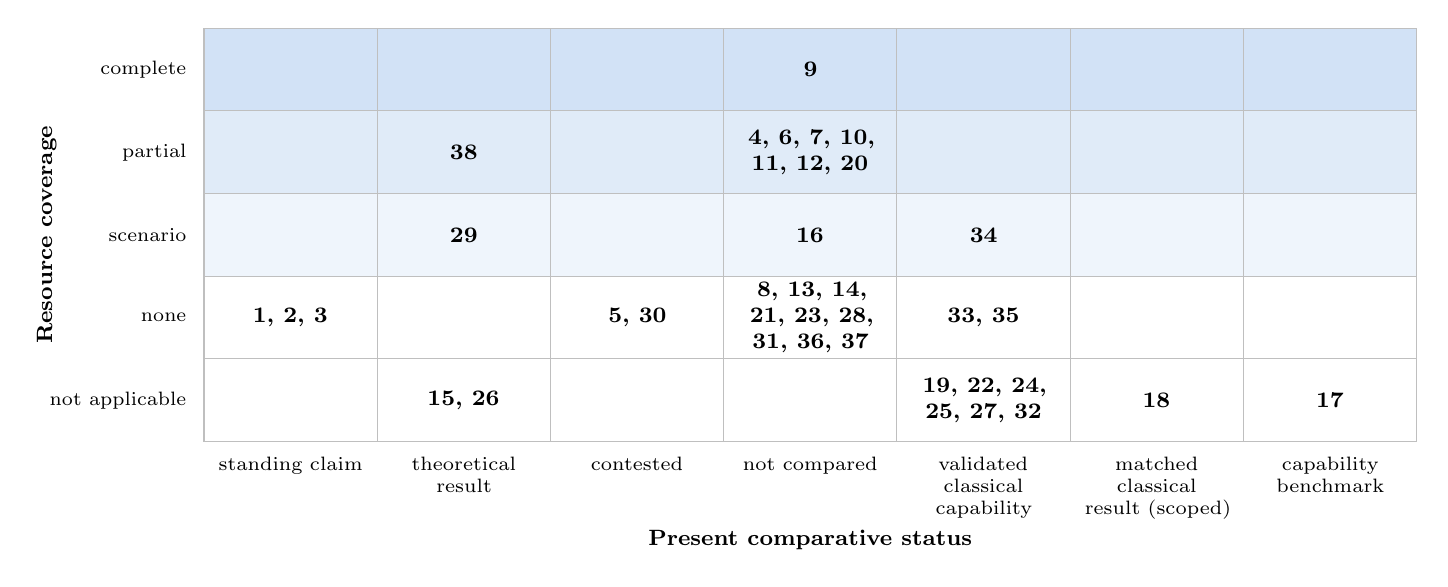
\begin{tikzpicture}[gridcell/.style={font=\footnotesize\bfseries, text width=2.0cm, align=center, inner sep=1pt}]
% background cells
\fill[qcF!20] (0,0) rectangle (15.4,-1.05);
\fill[qcF!14] (0,-1.05) rectangle (15.4,-2.1);
\fill[qcF!7] (0,-2.1) rectangle (15.4,-3.15);
\foreach \i in {0,...,6} {\foreach \j in {0,...,4} {
  \draw[black!25] (\i*2.2,-\j*1.05) rectangle ++(2.2,-1.05);
}}
% generated by ledger/make_figdata.py
\node[gridcell] at (1.100,-3.675) {1, 2, 3};
\node[gridcell] at (7.700,-1.575) {4, 6, 7, 10, 11, 12, 20};
\node[gridcell] at (5.500,-3.675) {5, 30};
\node[gridcell] at (7.700,-3.675) {8, 13, 14, 21, 23, 28, 31, 36, 37};
\node[gridcell] at (7.700,-0.525) {9};
\node[gridcell] at (3.300,-4.725) {15, 26};
\node[gridcell] at (7.700,-2.625) {16};
\node[gridcell] at (14.300,-4.725) {17};
\node[gridcell] at (12.100,-4.725) {18};
\node[gridcell] at (9.900,-4.725) {19, 22, 24, 25, 27, 32};
\node[gridcell] at (3.300,-2.625) {29};
\node[gridcell] at (9.900,-3.675) {33, 35};
\node[gridcell] at (9.900,-2.625) {34};
\node[gridcell] at (3.300,-1.575) {38};

% axis labels
\foreach \lab [count=\i from 0] in {standing claim, theoretical result, contested, not compared, validated classical capability, matched classical result (scoped), capability benchmark} {
  \node[font=\scriptsize, text width=2.05cm, align=center, anchor=north] at (\i*2.2+1.1,-5.32) {\lab};
}
\foreach \lab [count=\j from 0] in {complete, partial, scenario, none, not applicable} {
  \node[font=\scriptsize, anchor=east] at (-0.1,-\j*1.05-0.525) {\lab};
}
\node[font=\footnotesize\bfseries, anchor=north] at (7.7,-6.25) {Present comparative status};
\node[font=\footnotesize\bfseries, rotate=90, anchor=south] at (-1.75,-2.625) {Resource coverage};
\end{tikzpicture}}
\caption[Forward classes on two independent axes]{The \nClasses{} problem classes (numbers as in Table~\ref{tab:forward}) placed on two independent axes. The shading only separates the three coverage rows and carries no other meaning. Cell contents are generated from \texttt{forward\_classes.csv}. The ``not compared / partial'' cell holds resource-estimated candidates whose classical comparison is unresolved. The single entry in the top row is complete in coverage at the logical level, with unvalidated assumptions. No column means ``classical lead'': ``validated classical capability'' records a demonstrated classical result with no matched quantum workflow. Classes 34--35 are placed by their full-field sub-task. The classes are not independent units; several share sources, Hamiltonians or nested scopes, linked by the task-family field of the ledger, so the cell counts are counts of coded labels and not a survey statistic.}
\label{fig:grid}
\end{figure}
{\scriptsize
\setlength{\tabcolsep}{3pt}
\begin{longtable}{@{}r L{2.4cm} L{2.4cm} L{3.1cm} L{2.3cm} L{2.4cm} L{1.9cm}@{}}
\caption{Forward records for \nClasses{} problem classes (\texttt{forward\_classes.csv}). ``Resource evidence'' is in original units with coverage in brackets. The last three columns give the evidence that would favour the classical method ($\to$C), favour a quantum workflow ($\to$Q), or firm up the resource estimate ($\to$R). Each is a question that would change some assessment, not a sufficient condition for moving a whole class. Letter codes as in Fig.~\ref{fig:taxonomy}.}\label{tab:forward}\\
\toprule
\# & Class & Present status & Resource evidence [coverage] & $\to$C & $\to$Q & $\to$R\\
\midrule\endfirsthead
\toprule
\# & Class & Present status & Resource evidence [coverage] & $\to$C & $\to$Q & $\to$R\\
\midrule\endhead
\bottomrule\endfoot
1 & OTOC(2) scrambling, 2D & \psQ{} (\eld{E06} d), conditional & 65\,q measured; no FT compilation [\mtN] & Converged classical reproduction of the stated observable, depth and precision & Validated accuracy and full cost at larger scale & FT compilation\\
2 & Operator Loschmidt echo & \psQ, conditional & 56\,q measured [\mtN] & Majorana/Pauli propagation converged over the full regime & Bounded-error estimator costed for the same regime & FT compilation\\
3 & Floquet prethermal 2D magnetism: H2 and Heron instances & \psQ{} (\eld{E05} d; \eld{E23} d), two separate instances & 56\,q and 74\,q measured [\mtN] & Converged TN, NQS or Pauli-path result in the hardest regime of either instance & Validation across the hard regime, mitigation overhead costed & FT compilation\\
4 & 2D TFIM dynamics, 100 spins, 10 Trotter steps & \psN & 230 LQ, $2.4\times10^6$ T per execution [\mtP] & Converged classical result for the stated time, state and observable & Costed estimation below classical & Repetitions, preparation\\
5 & 3D spin-glass quenches & \psC{} (\mech{S}, \mech{V}), analog scope & Analog only [\mtN] & Stable long-time t-VMC or 3D BP-TN & Observables beyond classical coverage & Gate-model compilation\\
6 & 2D frustrated $J_1$--$J_2$ Heisenberg, $10\times10$ cylinder & \psN{} (baseline is 4-core DMRG) & $5.6\times10^4$\,s single factory [\mtP] & NQS, PEPS or GPU DMRG on the same cylinder at $\epsilon=0.01$ total, with measured cost & Validated adiabatic preparation & Gap scaling\\
7 & 2D Fermi--Hubbard energy, half filling & \psN{} (\mech{S}: sign-free; best classical baseline unresolved) & $1.05\times10^5$\,s at $10\times10$ vs 4-core DMRG $7.1\times10^9$\,s [\mtP] & QMC or parallel DMRG at $\epsilon=0.01$ total with measured time below the modelled schedule & Estimate below the best measured classical cost & Preparation\\
8 & Strongly correlated materials & \psN & No multi-orbital estimate [\mtN] & Downfolded classical solution at decision accuracy & Multi-orbital estimate with downfolding error and decision tolerance & Multi-orbital estimate\\
9 & Core-level XAS & \psN{} (resource-estimated candidate) & \xasCirc{} Toffoli longest circuit; \xasAlg{} total; \xasHours\,h at 1\,MHz [\mtC, assumptions unvalidated] & Classical spectrum at decision accuracy from the best available method & Validated preparation and error model, cost below that spectrum & Physical-level compilation\\
10 & FeMoco precision and other models & \psN & Dense code: \femoT\,h expected at \femoSevMinvolQ\,M physical, \femoTofMinvol{} Toffoli; THC $3.2\times10^{10}$ Toffoli [\mtP] & Classical estimate at matched confidence for larger models & Measured overlap; complete protocol & Larger-model counts\\
11 & P450 Cpd I spin gaps & \psN & 2022: $7.8\times10^9$ Toffoli, 73\,h; 2026: \pfMinvolH\,h at 1.03\,M physical [\mtP] & Converged classical spin gap at a stated tolerance & Cost for both spin states with error cancellation & Preparation, success criterion and both spin states on an architecture\\
12 & Ru CO$_2$-fixation catalysts & \psN & 2740 LQ, $5.4\times10^{11}$ T (older model); 56-orbital model 0.46\,h at 1.57\,M physical [\mtP] & Classical multireference result & Model-specific modern count & Modern count, older model\\
13 & Transition-metal ML labels & \psN & --- [\mtN] & Classical labels adequate & Incremental value of better labels against the downstream error budget & Label cost\\
14 & Enzyme active sites & \psN & No estimate for a named cluster [\mtN] & Embedding with a classical or neural solver adequate for a named cluster and observable & Solver error dominating a validated budget & Embedded estimates\\
15 & Learning from quantum data & \psT{} (quantum-side sample-complexity separation) & Separation with quantum memory~\cite{huang2022exp} [n/a] & Equivalent classical access model & Task demonstrations at scale & Copies, memory, access\\
16 & Real-time SU(3) gauge theory & \psN & $10^9$--$6.5\times10^{48}$ T across formulations, evolution only [\mtS] & Classical real-time method for a controlled physical observable & Controlled-truncation estimate incl.\ preparation and measurement & Single formulation, full observable\\
17 & Sampling capability: RCS, GBS, doped Clifford, analog atoms & \psCap & --- & --- & --- & ---\\
18 & SQD, single-layer circuit-energy objective & \psM{} (\mech{B}); workflow as a whole \psN & --- & --- & Sampler ablation under a common selection, recovery and diagonalization procedure & ---\\
19 & FeMoco-76 model energy & \psV{} (feasibility, extrapolation-dependent; operational ranking unresolved) & --- & --- & --- (a failed estimate would reopen the comparison) & ---\\
20 & P450 $\sim$500-orbital model & \psN & 9000 LQ, $1.5\times10^{12}$ Toffoli [\mtP] & Embedding solves the decision & A gap or decision target with a complete comparison & Modern count\\
21 & Generic ground-state chemistry & \psN & --- [\mtN] & --- & Representative family, fixed accuracy, with empirical or proven exponential classical scaling & ---\\
22 & Main-group thermochemistry & \psV{} (named benchmarks; \mech{R}) & --- & --- & Validated-domain failure with consequence (a solver need, not yet a quantum result) & ---\\
23 & Rydberg topological diagnostics & \psN & --- [\mtN] & --- & A matched computational task & Measurement cost\\
24 & High-throughput materials discovery & \psV{} (\mech{A}; experimentally validated~\cite{chen2024}) & --- & --- & Decision-critical electronic-structure bottleneck identified & Bottleneck estimate\\
25 & Binding free energies, MD & \psV{} (mature practice; \mech{A}); one unmatched hybrid workflow~\cite{merz2026} & --- & --- & Quantum subproblem dominating the budget, shown by ablation & Subproblem estimate\\
26 & Property learning within a phase & \psT{} (classical-side guarantee in theorem scope; \mech{A}) & --- & --- & Labels unobtainable classically & ---\\
27 & Protein structure prediction, proteome scale & \psV{} (\mech{R}); fragments are a separate record & --- & --- & Fragment gain under identical selection and cost rules & ---\\
28 & Generative molecular design & \psN & --- [\mtN] & Matched ablation shows no gain & Matched ablation incl.\ downstream selection shows gain & ---\\
29 & Unstructured search & \psT{} (conditional model; query-model limit~\cite{turturean2026}; \mech{H}) & Model only [\mtS] & --- & $t_Q\lesssim10\,\mu$s with $Q\gg1$ within a stated latency, or a structured speedup & Oracle estimate\\
30 & Approximate optimization: annealing (QAC) and Rydberg MIS & \psC, family-specific & QAC $>$1300 encoded variables; Rydberg $\le$289\,q [\mtN] & Classical portfolio matches scaling on the defined family & Separation vs the full portfolio with stated runtime accounting & ---\\
31 & QML on classical data & \psN & Constructed separations~\cite{liu2021} [\mtN] & --- & Practical separation on a stated workload and access model & ---\\
32 & Nuclear ground states, $A\le20$ & \psV{} (cited interactions; \mech{V}); no quantum comparator identified & --- & --- & A quantum comparator in scope at matched precision & ---\\
33 & Euclidean lattice QCD, zero density & \psV{} (mature practice); no demonstrated practical matched quantum advantage & Small-model sampling proposal~\cite{yamamoto2022} [\mtN] & --- & Lower autocorrelation and full observable cost than modern HMC at relevant lattice spacing & ---\\
34 & CFD: full field / selected outputs & \psV{} (full field: no costed quantum workflow) / selected outputs: see class 38 & Bounded advantage, modest for selected observables~\cite{jennings2025} [\mtS] & --- & Selected-observable workload with value and an end-to-end cost below explicit classical CFD & Selected-output estimate at an engineering Reynolds number\\
35 & Weather/climate: forecasts / statistics & \psV{} per named forecast or component / \psN & --- [\mtN] & --- & A named component with a costed advantage & Component estimate\\
36 & Doped 2D Fermi--Hubbard (sign-problem instances) & \psN{} (new record) & --- [\mtN] & NQS, PEPS, constrained-path or embedding result at stated density, $U/t$, $t'$ and tolerance, with measured cost & Costed QPE estimate for the same instance & Doped-lattice estimate\\
37 & Quantum-enhanced MCMC sampling & \psN{} (conditional candidate) & Proposals and early hardware experiments~\cite{layden2023,marshall2026} [\mtN] & Classical nonlocal updates matching time per independent sample & Lower time per independent sample incl.\ proposal generation and noise & Proposal circuit cost\\
38 & Sparse linear solves and time stepping for engineering PDEs (FEM, CFD) & \psT{} (at most polynomial speedup in fixed dimension~\cite{montanaro2016}; \mech{IO}, \mech{H}) & $10^{21}$--$10^{39}$ logical qubits $\times$ T gates for drag on a sphere~\cite{penuel2025}; depth $1.8\times10^{29}$ for EM scattering~\cite{scherer2017}; one crossover at $2^{80}$ grid points~\cite{zhuang2025} [\mtP] & --- (classical practice is the incumbent) & A high-dimensional or quantum-native linear problem with scalar output and an end-to-end cost below tuned multigrid or Monte Carlo & Constant-factor estimate at industrial condition numbers with input and readout\\
\end{longtable}
}

% =====================================================================
\section{Resource models, records and further figures}
\label{app:models}

\paragraph{Rows shown in Fig.~\ref{fig:dc76}.} The rows are from Table~XXVII of the dense-code compilation (physical error rate $10^{-3}$, 1\,$\mu$s code cycle, 10\,$\mu$s reaction time). From left to right: the minimum-qubit row, the rows the source highlights as running within a month and within a day, the minimum-volume row and the fastest tabulated row; for FeMoco a second fast row at \femoSevSelQ\,M qubits is also shown. The vertical axis is the source's expected runtime, which is the one-shot runtime divided by one minus the logical failure probability (its Sec.~VI.B). At the low-qubit end most shots fail: the minimum-qubit FeMoco row has a failure probability of \femoMinqPfail, so \femoMinqShot{} hours per shot become \femoMinqH{} expected hours. Spectral-hit repetitions, state preparation and the second spin state needed for a P450 gap are not included, and classical reference values are given in the text with their own scopes.

\subsection{Runtime bounds and implied rates}
In general a fault-tolerant execution is bounded below by its slowest required resource stream,
\begin{equation}
T_{\rm run}\ \gtrsim\ \max\!\left\{\frac{N_T}{R_T},\ \frac{N_{\rm CCZ}}{R_{\rm CCZ}},\ D_{\rm adapt}\,t_{\rm react},\ D_{\rm code}\,t_{\rm cycle},\ T_{\rm routing/readout}\right\},
\label{eq:bottleneck}
\end{equation}
where $R_T$ and $R_{\rm CCZ}$ are the production rates of T and CCZ states, $D_{\rm adapt}$ the number of sequential reaction-dependent stages and $D_{\rm code}$ the logical depth in code cycles. State preparation, resets and outer repetitions come on top. Inverting published estimates gives the effective rates of Fig.~\ref{fig:rates}. A complete execution record would list
$(Q_{\rm data}, Q_{\rm work}, Q_{\rm factory}, N_{\rm T}, N_{\rm CCZ}, D_{\rm adapt}, p_{\rm fail}, t_{\rm cycle}, t_{\rm react})$; most published estimates report a subset.

\begin{figure}[htbp]
\centering
\begin{tikzpicture}
\begin{axis}[
  xbar, xmode=log, log origin=infty, width=0.66\textwidth, height=6.6cm,
  xmin=10, xmax=2e7, y dir=reverse, ytick={1,...,8}, ymin=0.4, ymax=8.6,
  yticklabels={{TFIM, ns gates, $p{=}10^{-4}$}, {TFIM, ns gates, $p{=}10^{-3}$}, {Ru catalyst, ns, $p{=}10^{-4}$}, {Ru catalyst, ns, $p{=}10^{-3}$}, {TFIM, $\mu$s gates, $p{=}10^{-4}$}, {Ru catalyst, $\mu$s, $p{=}10^{-4}$}, {P450 model X, THC, $p{=}10^{-3}$}, {FeMoco-54, THC, 4\,M phys.}},
  yticklabel style={font=\footnotesize},
  xlabel={\footnotesize Effective non-Clifford rate $N/T$ (states per second)},
  xticklabel style={font=\footnotesize}, bar width=7pt, bar shift=0pt,
  xmajorgrids, grid style={black!10},
  nodes near coords={\pgfmathprintnumber[sci,precision=1]{\pgfplotspointmeta}}, point meta=x, every node near coord/.append style={font=\scriptsize, anchor=west},
  axis x line*=bottom, axis y line*=left,
  legend style={font=\scriptsize, at={(0.98,0.03)}, anchor=south east, draw=black!25, fill=white}]
\addplot[fill=qcF, draw=none] table[x=x,y=y] {figdata/rates_T.dat};
\addlegendentry{T states (Beverland et al.)}
\addplot[fill=black!20, draw=black!75, line width=0.3pt, postaction={pattern=north east lines, pattern color=black!80}] table[x=x,y=y] {figdata/rates_CCZ.dat};
\addlegendentry{Toffoli/CCZ}
\end{axis}
\end{tikzpicture}
\caption[Rates implied by particular schedules]{Effective non-Clifford rates $N/T$ implied by particular published schedules, from \texttt{resources.csv}. T-state and Toffoli rates are different quantities and are drawn with different fills (plain bars for T states, hatched bars for Toffoli gates); the validator refuses a Toffoli record in the T series. Each value belongs to its source schedule (factory count, code, width, gate speed) and is not a portable platform performance. Sources: TFIM and Ru catalyst~\cite{beverland2022}; P450, $7.8\times10^9$ Toffoli in 73\,h~\cite{goings2022}; FeMoco 54-orbital layout, $6.7\times10^9$ Toffoli in 3 days at a stated 25\,kHz~\cite{lee2021thc}.}
\label{fig:rates}
\end{figure}

\subsection{Comparison with announced hardware targets}
\label{app:vendor}
Public hardware roadmaps provide scale references, not application schedules (Table~\ref{tab:vendor}). T counts, Toffoli counts and vendor ``operations'' are different units, and the vendor unit is not defined in the announcements. We therefore compare only under a named accounting convention and draw only one-sided conclusions about named compiled circuits.

\begin{rulebox}{Convention X and bound logic}
\textbf{Convention X (illustrative):} one vendor operation implements at most one counted non-Clifford gate (T or CCZ alike), with Clifford, routing and memory operations free. This is an accounting convention, not a property of any architecture. A source circuit's count is not a lower bound on every circuit for the same task.
\begin{itemize}
\item If a \emph{named compiled circuit} has count $N\ge L$ and $L>B$, that circuit does not fit budget $B$ under convention X or any costlier one: a count obstruction for that circuit.
\item If $N\le U$ and $U\le B$, the count is within $B$ under convention X only; compatibility with a real architecture is \emph{not established}.
\item A workload of many independent circuits is tested one circuit at a time. A cumulative count is comparable only with a cumulative budget, which the announcements do not state.
\item A compiled width above the announced logical-qubit count, under the same width convention, is a width obstruction as compiled. A record with no reported width has unknown compatibility.
\end{itemize}
\end{rulebox}
Logical error and circuit volume must also agree. Under an independent-failure model with failure probability $p_L$ per counted operation, $P(\text{success})\approx e^{-Gp_L}$, so $G=10^8$ operations at 99\% success need $p_L\lesssim10^{-10}$ and $G=10^9$ need $p_L\lesssim10^{-11}$.

\begin{table}[htbp]
\centering\small
\caption{Announced vendor targets used as scale references. Targets are forward-looking statements, not delivery commitments.}\label{tab:vendor}
\begin{tabular}{@{}L{3.1cm} L{1.6cm} L{2.4cm} L{2.3cm} L{5.0cm}@{}}
\toprule
System & Target date & Logical qubits & Logical operations & Error target and implied success\\\midrule
IBM Starling~\cite{ibmroadmap2025} & 2029 & 200 & $10^8$ & Unit not specified in announcement; $10^8$ ops at 99\% success implies $p_L\lesssim10^{-10}$\\
IBM Blue Jay~\cite{ibmroadmap2025,hpcwire2025} & 2033+ & 2000 & $10^9$ & As above; implies $p_L\lesssim10^{-11}$\\
Quantinuum Apollo~\cite{quantinuum2024,quantFiling} & 2029 & hundreds & not stated as an operation count & Logical fidelity target ``Ten Nines'', error as low as $\sim10^{-10}$ per filing\\
\bottomrule
\end{tabular}
\end{table}
\begin{figure}[htbp]
\centering
\begin{tikzpicture}
\begin{axis}[
  xmode=log, ymode=log, width=0.82\textwidth, height=8.2cm,
  xmin=60, xmax=1e5, ymin=1e6, ymax=1e13,
  xlabel={\footnotesize Logical qubits, in each source's width convention}, ylabel={\footnotesize Non-Clifford count in source unit},
  ticklabel style={font=\footnotesize}, grid=major, grid style={black!10}, clip=false,
  legend style={font=\scriptsize, at={(0.5,-0.16)}, anchor=north, draw=black!25, fill=white, legend columns=2}, legend cell align=left]
\draw[dashed, draw=qcQ, line width=0.8pt] (axis cs:60,1e8) -- (axis cs:200,1e8) -- (axis cs:200,1e6);
\draw[dashed, draw=qcQ, line width=0.8pt] (axis cs:60,1e9) -- (axis cs:2000,1e9) -- (axis cs:2000,1e6);
\node[font=\scriptsize, qcQ, anchor=west] at (axis cs:62,2.5e7) {200 LQ / $10^8$ ops};
\node[font=\scriptsize, qcQ, anchor=south west] at (axis cs:62,1.15e9) {2000 LQ / $10^9$ ops (IBM targets, per circuit)};
\addplot[only marks, mark=*, mark size=2.6pt, color=qcF] table[x=x,y=y] {figdata/resmap_T_point.dat};
\addlegendentry{T count, one circuit}
\addplot[only marks, mark=triangle*, mark size=3.2pt, color=black!70] table[x=x,y=y] {figdata/resmap_Toff_point.dat};
\addlegendentry{Toffoli count, one circuit}
% generated by ledger/make_figdata.py
\node[font=\scriptsize, inner sep=5pt, anchor=west] at (axis cs:230,2.4e6) {2D TFIM dynamics, per execution};
\node[font=\scriptsize, inner sep=5pt, anchor=north] at (axis cs:2740,5.4e11) {Ru CO$_2$ catalyst};
\node[font=\scriptsize, inner sep=5pt, anchor=west] at (axis cs:25481,1.5e10) {RSA-2048};
\node[font=\scriptsize, inner sep=5pt, anchor=west] at (axis cs:100,3.54e8) {XAS, longest circuit (min.\ workspace)};
\node[font=\scriptsize, inner sep=5pt, anchor=north west] at (axis cs:2142,5.3e9) {FeMoco-54 (Reiher), THC};
\node[font=\scriptsize, inner sep=5pt, anchor=west] at (axis cs:2196,3.2e10) {FeMoco-76 (Li), THC};
\node[font=\scriptsize, inner sep=5pt, anchor=south east] at (axis cs:9000,1.5e12) {P450 $\sim$500-orbital model};

\end{axis}
\end{tikzpicture}
\caption[Single-circuit resource estimates and announced vendor targets]{Published single-circuit resource estimates in their original units; only records read at table or section level with a reported compiled width are shown. Dashed lines are announced IBM targets, drawn as reference lines and not as feasibility regions. By the bound logic of Appendix~\ref{app:vendor}, a point beyond a line is an obstruction for that compiled circuit under convention X; a point inside a line establishes nothing about a real architecture. The XAS point is the longest circuit at the minimum algorithm workspace of 100 logical qubits, excluding factories~\cite{fomichev2025}. Cumulative counts over many circuits, such as the \xasAlg{} Toffoli gates of the full XAS spectrum, are not comparable with a per-circuit budget and are not drawn. The two FeMoco points are different Hamiltonians~\cite{lee2021thc}. Records without a reported width (lattice models, dense-code compilations, most gauge formulations) are omitted. Sources: TFIM, Ru, RSA~\cite{beverland2022}; P450~\cite{goings2022}.}
\label{fig:resource}
\end{figure}

\subsection{Break-even and output scenarios}
Fig.~\ref{fig:quadratic} plots Eq.~(\ref{eq:tstar}). The cubic and quartic curves are sensitivities for hypothetical structured algorithms (\beCubic\,s and \beQuartic\,s at $t_Q=1$\,ms and $P=10^6$); they are not known search algorithms.

\begin{figure}[htbp]
\centering
\begin{tikzpicture}
\begin{axis}[
  xmode=log, ymode=log, width=0.56\textwidth, height=6.4cm,
  xmin=1, xmax=1e7, ymin=1e-3, ymax=1e10,
  xlabel={\footnotesize Effective classical parallelism $P$ (cores)},
  ylabel={\footnotesize Break-even runtime $T^*$ (s)},
  ticklabel style={font=\footnotesize}, grid=major, grid style={black!10},
  legend style={font=\scriptsize, at={(1.04,0.5)}, anchor=west, draw=black!25, fill=white}, legend cell align=left]
\addplot[qcF, line width=1.3pt, mark=*, mark size=1.8pt, mark repeat=5] table[x=P,y=d2ms] {figdata/breakeven_curves.dat};
\addlegendentry{$d=2$, $t_Q=1$\,ms, $Q=1$}
\addplot[qcF!75, line width=1.0pt, mark=square*, mark size=1.7pt, mark repeat=5, mark phase=2] table[x=P,y=d2hundred] {figdata/breakeven_curves.dat};
\addlegendentry{$d=2$, $t_Q=100\,\mu$s, $Q=1$ (= 1\,ms, $Q=100$)}
\addplot[qcF!55, line width=1.0pt, mark=triangle*, mark size=2.2pt, mark repeat=5, mark phase=4] table[x=P,y=d2ten] {figdata/breakeven_curves.dat};
\addlegendentry{$d=2$, $t_Q=10\,\mu$s, $Q=1$}
\addplot[black!60, line width=1.0pt, dashed] table[x=P,y=d3ms] {figdata/breakeven_curves.dat};
\addlegendentry{hypothetical $d=3$, $t_Q=1$\,ms}
\addplot[black!60, line width=1.0pt, dotted] table[x=P,y=d4ms] {figdata/breakeven_curves.dat};
\addlegendentry{hypothetical $d=4$, $t_Q=1$\,ms}
\draw[black!40, dashed] (axis cs:1,86400) -- (axis cs:1e7,86400) node[pos=0.02, above, font=\scriptsize, anchor=south west]{1 day};
\draw[black!40, dashed] (axis cs:1,3.16e7) -- (axis cs:1e7,3.16e7) node[pos=0.02, above, font=\scriptsize, anchor=south west]{1 year};
\node[circle, fill=qcF, inner sep=1.5pt] at (axis cs:1e6,1e8) {};
\node[font=\scriptsize, anchor=east, inner sep=5pt] at (axis cs:1e6,1e8) {3.2 y};
\node[circle, fill=qcF!70, inner sep=1.5pt] at (axis cs:1e6,1e6) {};
\node[font=\scriptsize, anchor=west, inner sep=5pt] at (axis cs:1e6,1e6) {11.6 d};
\node[circle, fill=qcF!45, inner sep=1.5pt] at (axis cs:1e6,10000) {};
\node[font=\scriptsize, anchor=west, inner sep=5pt] at (axis cs:1e6,10000) {2.8 h};
\node[circle, fill=black!60, inner sep=1.5pt] at (axis cs:1e6,4.64159) {};
\node[font=\scriptsize, anchor=north, inner sep=5pt] at (axis cs:1e6,4.64159) {4.6 s};

\end{axis}
\end{tikzpicture}
\caption[Break-even runtime for polynomial speedups]{Break-even runtime $T^*$ (Eq.~\ref{eq:tstar}) with $t_C=10$\,ns per equivalent oracle evaluation; a formula figure whose parameters are in \texttt{models.csv}. Solid lines with markers are the quadratic case (circles, squares and triangles mark the three gate times of the legend), which corresponds to unstructured search. Dashed and dotted lines are model sensitivities for hypothetical structured algorithms of higher degree, not known search algorithms. The model assumes equivalent oracle work on both sides, effective parallelism $P$, a problem that partitions across $Q$ quantum processors, and reaction-dependent stages that set $t_Q$. No acceptable-latency threshold is implied.}
\label{fig:quadratic}
\end{figure}

For output, suppose a receiver needs $N$ values of $b$ bits that are independent of everything it already holds, obtained from fresh preparations of an $n$-qubit state. Each shot yields at most $n$ classical bits, so
\begin{equation}
T^{\rm out}_Q \;\ge\; \frac{N\,b\,t_{\rm shot}}{n\,Q},\qquad T^{\rm out}_C \;\approx\; \frac{N\,b}{B_{\rm mem}},
\label{eq:output}
\end{equation}
for $Q$ quantum devices and a classical memory bandwidth $B_{\rm mem}$. With $N=10^9$, $b=32$, $n=10^3$, $t_{\rm shot}=1$\,ms and $B_{\rm mem}=10^{12}$\,bits/s the floor is \outQ\,s per quantum device against \outC\,s of classical writing (Fig.~\ref{fig:readout}). The scenario is a conditional floor for one information model. A simulated field is a deterministic function of its inputs, so it need not carry $Nb$ bits of new information; a smooth field has a short description; and an algorithm that outputs selected observables is not subject to the floor.

\begin{figure}[htbp]
\centering
\begin{tikzpicture}
\begin{axis}[
  xmode=log, ymode=log, width=0.66\textwidth, height=6.0cm,
  xmin=1e6, xmax=1e21, ymin=1e-6, ymax=1e18,
  xlabel={\footnotesize Independent information to deliver: $N$ values of 32 bits},
  ylabel={\footnotesize Output time (s)},
  ticklabel style={font=\footnotesize}, grid=major, grid style={black!10},
  legend style={font=\scriptsize, at={(0.02,0.98)}, anchor=north west, draw=black!25, fill=white}, legend cell align=left]
\addplot[qcF, line width=1.2pt] table[x=N,y=q_ms] {figdata/readout_curves.dat};
\addlegendentry{quantum floor, $n=10^3$, $t_{\rm shot}=1$\,ms}
\addplot[qcF!55, line width=1.1pt, dashed] table[x=N,y=q_us] {figdata/readout_curves.dat};
\addlegendentry{quantum floor, $n=10^3$, $t_{\rm shot}=1\,\mu$s}
\addplot[black!75, line width=1.2pt, dashdotted] table[x=N,y=c_node] {figdata/readout_curves.dat};
\addlegendentry{classical node, $10^{12}$ bits/s}
\draw[black!40, dashed] (axis cs:1e6,86400) -- (axis cs:1e21,86400) node[pos=0.98, above, anchor=south east, font=\scriptsize]{1 day};
\draw[black!40, dashed] (axis cs:1e6,3.16e7) -- (axis cs:1e21,3.16e7) node[pos=0.98, above, anchor=south east, font=\scriptsize]{1 year};
\end{axis}
\end{tikzpicture}
\caption[Output time under an information-rate scenario]{An information-rate scenario for output (Eq.~\ref{eq:output}): time to deliver $N$ independent 32-bit values from one quantum device by fresh preparations of a 1{,}000-qubit state, against writing them on one classical node. The scenario assumes that the receiver holds no information that shortens the description, which a deterministic simulated field need not satisfy. The curves exclude the solve on both sides, do not rank total runtimes and do not apply to algorithms that output selected observables. A formula figure; parameters in \texttt{models.csv}.}
\label{fig:readout}
\end{figure}

\subsection{Resource records}
{\scriptsize
\setlength{\tabcolsep}{3pt}
\begin{longtable}{@{}L{2.5cm} L{1.15cm} L{1.55cm} L{2.85cm} L{3.0cm} L{3.05cm} L{0.95cm}@{}}
\caption{Resource records used in this paper, one per model, algorithm and schedule (\texttt{resources.csv}). LQ = logical qubits as compiled unless stated. ``Capability'' applies the bound logic of Appendix~\ref{app:vendor} under convention X to the named circuit against the IBM targets (200 LQ / $10^8$; 2000 LQ / $10^9$). Coverage: \mtC{} = preparation, observable, repetitions and error budget costed for the stated protocol; \mtP{} = listed omissions; \mtS{} = evolution-only or truncation-dependent. Coverage says nothing about whether the assumptions are validated. Rows marked $\ddagger$ carry a value known at second hand or from an abstract only; no such value is used in a figure or ratio. $^\S$n.c.\ = not constructed: the dense-code source tabulates compute, hot-storage and cold-storage regions separately, and we do not add them into a logical width.}\label{tab:worked}\\
\toprule
Record & LQ & $N_{\rm nc}$ & Quantum time & Classical time & Capability (convention X) & Cov.\\
\midrule\endfirsthead
\toprule
Record & LQ & $N_{\rm nc}$ & Quantum time & Classical time & Capability (convention X) & Cov.\\
\midrule\endhead
\bottomrule\endfoot
2D TFIM dynamics, 100 spins, 10 steps~\cite{beverland2022} & 230 & $2.4\times10^6$ T & 0.56\,s per execution (ns, $p{=}10^{-4}$); repetitions excluded & No current baseline compiled & Width obstruction vs 200 as compiled; count within $10^8$ under X only & \mtP\\
Fermi--Hubbard $6\times6$ cylinder, $U/t{=}4$, half filling, $\epsilon=0.01$ total~\cite{yoshioka2024} & 72 (system) & not reported & $1.23\times10^4$\,s (1 factory, $4.3\times10^5$ physical); $1.59\times10^3$\,s (16 factories, $3.4\times10^6$) & DMRG $2.2\times10^5$\,s on 4 cores (est.); QMC sign-free, not costed & --- & \mtP\\
Fermi--Hubbard $10\times10$, same~\cite{yoshioka2024} & 200 (system) & not reported & $1.05\times10^5$\,s (1 factory, $8.9\times10^5$ physical); $1.46\times10^4$\,s (16 factories, $5.4\times10^6$) & DMRG $7.1\times10^9$\,s on 4 cores (est.) = \hubTenCoreH{} core-h; QMC not costed & --- & \mtP\\
$J_1$--$J_2$ Heisenberg $10\times10$ cylinder, $J_2/J_1{=}0.5$~\cite{yoshioka2024} & 100 (system) & not reported & $5.64\times10^4$\,s (1 factory, $5.1\times10^5$ physical); $4.32\times10^3$\,s (16 factories, $4.4\times10^6$) & DMRG $7.9\times10^4$\,s on 4 cores (est.); NQS on another geometry: 4 d on 20 GPUs~\cite{rende2024} & --- & \mtP\\
XAS, Li$_4$Mn$_2$O, CAS(22e,18o)~\cite{fomichev2025}: longest circuit & 100 (min.\ work\-space, excl.\ factories) & \xasCirc{} Toffoli & \xasCircS\,s at a 1\,MHz logical clock ($1.08\times10^8$ cycles) & --- & Width within 200 by that convention; count obstruction vs $10^8$ for this circuit; within $10^9$ under X only & \mtC\\
XAS, same: full sampled spectrum & 350 (active-volume implementation) & \xasAlg{} Toffoli over all circuits & \xasHours\,h at 1\,MHz (source: less than two days) & RAS: $\sim$32 days for 1{,}000 states (source's estimate, which it calls likely optimistic on the classical side) & Cumulative count; not comparable with a per-circuit budget & \mtC\\
FeMoco, 76 orbitals, THC~\cite{lee2021thc} & 2196 & $3.2\times10^{10}$ Toffoli & no physical layout in the source & --- & Count obstruction vs $10^9$ for this algorithm & \mtP\\
FeMoco, 54 orbitals, THC~\cite{lee2021thc} & 2142 & $5.3\times10^9$ Toffoli ($6.7\times10^9$ in the layout) & 3 days at 25\,kHz on 4\,M physical (abstract: under four days) & --- & Count obstruction vs $10^9$ for this algorithm & \mtP\\
FeMoco, 76 orbitals, dense code, minimum volume~\cite{low2026dense} & n.c.$^\S$ & \femoTofMinvol{} Toffoli & \femoT\,h expected (\femoShot\,h per shot, $p_{\rm fail}=\femoPfail$), \femoSevMinvolQ\,M physical & Three classical records (Section~\ref{sec:chem}) & Count obstruction vs $10^9$ for this compilation & \mtP\\
FeMoco, 76 orbitals, dense code, fastest tabulated~\cite{low2026dense} & n.c.$^\S$ & \femoTofFast{} Toffoli & \femoFastT\,h expected, \femoSevFastQ\,M physical & as above & Count obstruction vs $10^9$ & \mtP\\
FeMoco, 76 orbitals, dense code, within a month~\cite{low2026dense} & n.c.$^\S$ & $1.49\times10^{10}$ Toffoli & 716\,h expected (529\,h per shot, $p_{\rm fail}=\femoLowPfail$), \femoSevLowQ{} physical & as above & Count obstruction vs $10^9$ & \mtP\\
FeMoco, 76 orbitals, spectrum amplification (count)~\cite{low2025sa} & 1459 & $9.99\times10^8$ Toffoli per run & no physical layout with this count & --- & Width within 2000; count within $10^9$ under X only, with no margin & \mtP\\
FeMoco, 54 orbitals, spectrum amplification (count)~\cite{low2025sa} & 1137 & $3.41\times10^8$ Toffoli per run & no physical layout with this count & --- & Width within 2000; count within $10^9$ under X only & \mtP\\
FeMoco, 76 orbitals, spectrum amplification (schedule)$^\ddagger$~\cite{low2025sa,zhai2026} & not extracted & not extracted & 8.6\,h per attempt, four CCZ factories, $\sim$4.5\,M physical & --- & --- & \mtP\\
FeMoco, candidate-refinement protocol~\cite{berry2024} & not extracted & $7.3\times10^{10}$ Toffoli (2 or 3 phase-estimation rounds; 2.3 times the single-shot THC count) & --- & --- & Count obstruction vs $10^9$ & \mtP\\
FeMoco, 76 orbitals, classical campaign~\cite{zhai2026} & --- & --- & --- & 2.77\,M core-h measured; $\pm$0.31/$\pm$1.25 kcal/mol & --- & ---\\
FeMoco, 54 orbitals, dense code, minimum volume~\cite{low2026dense} & n.c.$^\S$ & $4.55\times10^8$ Toffoli & 1.13\,h expected, 1.15\,M physical (Fig.~\ref{fig:femoco}) & --- & Within $10^9$ under X only & \mtP\\
P450 Cpd I model X, 2022~\cite{goings2022} & not reported$^\dagger$ & $7.8\times10^9$ Toffoli & 73\,h on 4.6\,M physical ($p{=}10^{-3}$); 25\,h on 0.5\,M ($10^{-5}$) & DMRG $M{=}3000$: 36{,}564 CPU-h, $\sim$1 month (both estimated in source) & Count obstruction vs $10^9$ for this algorithm & \mtP\\
P450 Cpd I model X (58o63e), dense code, 2026~\cite{low2026dense} & n.c.$^\S$ & \pfTofMinvol{} (minimum volume); \pfTofFast{} (fastest) Toffoli & \pfMinvolH\,h at 1.03\,M physical; \pfFastH\,h at 2.18\,M; \pfMinqDays{} days at 81{,}000 & as above & Within $10^9$ under X only & \mtP\\
P450 $\sim$500-orbital model~\cite{goings2022} & 9000 & $1.5\times10^{12}$ Toffoli & --- & --- & Width and count obstructions & \mtP\\
Ru CO$_2$-fixation catalyst~\cite{beverland2022} & 2740 & $5.4\times10^{11}$ T & 1 month (ns); 130\,y ($\mu$s) & Not reported & Width and count obstructions for this circuit & \mtP\\
Ru catalyst XVIII, 56o64e (another active space), dense code~\cite{low2026dense} & n.c.$^\S$ & $2.25\times10^8$ Toffoli (fastest row); $5.55\times10^9$ (minimum qubits) & 0.46\,h at 1.57\,M physical; 3{,}200\,h at 76{,}000 & Not reported & --- & \mtP\\
EM scattering by finite elements, $3.3\times10^8$ unknowns~\cite{scherer2017} & $\sim10^8$ (width incl.\ oracles) & depth $1.8\times10^{29}$; T-depth $8.2\times10^{28}$ & --- & big-O comparison only & Width and count obstructions & \mtP\\
Drag on a sphere, Carleman lattice Boltzmann$^\ddagger$~\cite{penuel2025} & \multicolumn{2}{L{3.0cm}}{$10^{21}$--$10^{39}$ logical qubits $\times$ T gates} & --- & steady RANS on one workstation, 1--10\,h for $\mathrm{Re}=10^3$--$10^7$ (source's reference); explicit CFD scales as $O(\mathrm{Re}^3)$ & not assessed (abstract-level value) & \mtP\\
Navier--Stokes, $2^{80}$-point mesh~\cite{zhuang2025} & 181 & $9.41\times10^7$ Toffoli and $3.94\times10^8$ rotations per preparation; 1{,}000 preparations & 42.6 days, 8.71\,M physical (94\% factories), distance 25 & 130 years: banded-Cholesky operation count for the full system at a benchmark rate & Width within 200; count within $10^8$ per preparation under X only & \mtP\\
Drag on a sphere, public per-instance records~\cite{qsub2025}: $\mathrm{Re}=10$ and $10^8$ & 5{,}679; $8.6\times10^{10}$ & $9.3\times10^{17}$; $9.2\times10^{29}$ T & --- & as above & not assessed (unreconciled with the published range) & \mtP\\
SU(3) shear viscosity, $\Sigma(72\times3)$ subgroup~\cite{osorio2025} & 27{,}000 (data registers only) & $3.5\times10^{12}$ T (Kogut--Susskind); $7.1\times10^{12}$ T (improved) & evolution only & as below & Width and count obstructions & \mtS\\
SU(3) plaquette block encoding, one oracle~\cite{draper2026} & not a total width & $1.2\times10^5$ T ($B{=}6$); $1.2\times10^6$ T ($B{=}9$) & subroutine only & --- & not an application count & \mtS\\
SU(3) shear viscosity, $10^3$: separate formulations (Fig.~\ref{fig:lgt})~\cite{lamm2026,ciavarella2025} & per formulation; mostly not reported & $10^9$ to $6.5\times10^{48}$ T & evolution only & No scalable classical route known for the full theory & The one record with a width does not fit; unknown where no width is reported & \mtS\\
Unstructured search~\cite{babbush2021,hoefler2023} & any & $\sqrt{M/Q}$ calls & Eq.~(\ref{eq:tstar}) & $Mt_C/P$ & --- & \mtS\\
RSA-2048 (reference)~\cite{beverland2022} & 25{,}481 & $1.5\times10^{10}$ T & 18\,h ($10^{-4}$, ns) & --- & Width and count obstructions & ref.\\
\end{longtable}
}
\noindent{\scriptsize $^\dagger$A secondary summary lists $\sim$4{,}900 logical qubits; not confirmed in the primary source and not used.}

\subsection{Further figures for the chemistry, lattice and gauge cases}
Fig.~\ref{fig:femoco} shows the frontier for the smaller FeMoco model and its history. Fig.~\ref{fig:sqd} gives the sampling limits of quantum-selected configuration interaction discussed in Section~\ref{sec:devices}. Fig.~\ref{fig:dmrg} shows how DMRG cost grows with bond dimension for the P450 models: with CPU time growing as the cube of the bond dimension, a value of 12{,}000 would cost \planCoreH{} core-hours and about \planMemTB\,TB of memory, a budget available at supercomputer scale, although whether that bond dimension converges the spin gap is a separate and empty evidence field. Fig.~\ref{fig:platform} shows how one fixed algorithm depends on the hardware scenario, and Fig.~\ref{fig:lgt} the spread of gauge-theory estimates.

\begin{figure}[htbp]
\centering
\begin{tikzpicture}
\begin{groupplot}[group style={group size=2 by 1, horizontal sep=1.9cm}, height=6.0cm, ticklabel style={font=\footnotesize}, label style={font=\footnotesize}]
\nextgroupplot[width=0.56\textwidth, xmode=log, ymode=log, xmin=4e4, xmax=1.5e7, ymin=0.3, ymax=5000, xlabel={Physical qubits}, ylabel={Expected runtime (hours)}, grid=major, grid style={black!10}, clip=false]
\addplot[only marks, mark=square*, mark size=2.6pt, color=black!55] table[x=x,y=y] {figdata/femoco54_prior.dat};
\addplot[only marks, mark=*, mark size=2.8pt, color=qcF] table[x=x,y=y] {figdata/femoco54_dense.dat};
\addplot[qcF!60, dashed] table[x=x,y=y] {figdata/femoco54_dense.dat};
\node[font=\scriptsize, anchor=west] at (axis cs:6.3e6,1440) {DF};
\node[font=\scriptsize, anchor=west] at (axis cs:4.2e6,72) {THC};
\node[font=\scriptsize, anchor=west] at (axis cs:3.4e6,3) {DFTHC+SA};
\node[font=\scriptsize, anchor=south west, qcF] at (axis cs:9.5e4,720) {compact};
\node[font=\scriptsize, anchor=north east, qcF] at (axis cs:1.9e5,20) {balanced};
\node[font=\scriptsize, anchor=north east, qcF] at (axis cs:1.0e6,1.0) {efficient};
\node[font=\scriptsize, anchor=north west, qcF] at (axis cs:2.1e6,0.75) {fast};
\draw[{Latex[length=2mm]}-{Latex[length=2mm]}, black!50] (axis cs:88840,2.2) -- node[below, font=\scriptsize]{36$\times$ fewer qubits} (axis cs:3.2e6,2.2);

\nextgroupplot[width=0.40\textwidth, ybar, ymode=log, log origin=infty, ymin=0.5, ymax=2e4, xtick={1,...,7}, xticklabels={DF,THC,DFTHC,compact,balanced,efficient,fast}, xmin=0.4, xmax=7.6, xticklabel style={rotate=45, anchor=east, font=\scriptsize}, ylabel={Space-time volume ($10^6$ qubit-h)}, bar width=8pt, bar shift=0pt, nodes near coords, point meta=rawy, every node near coord/.append style={font=\tiny}]
\addplot[fill=black!20, draw=black!75, line width=0.3pt, postaction={pattern=north east lines, pattern color=black!80}] table[x=x,y=y] {figdata/femoco54vol_prior.dat};
\addplot[fill=qcF, draw=none] table[x=x,y=y] {figdata/femoco54vol_dense.dat};
\end{groupplot}
\end{tikzpicture}
\caption[FeMoco, 54 orbitals: quantum cost frontier]{Phase estimation on the 54-orbital FeMoco model at 1\,mHa, all values from one source~\cite{low2026dense}. Squares, and hatched bars in the right panel: prior estimates as tabulated there, by double factorization (DF), tensor hypercontraction (THC) and THC with spectrum amplification (DFTHC+SA). Circles and plain bars: the 2026 dense planar surface code at a 1\,$\mu$s cycle and 10\,$\mu$s reaction time, in four rows of its Table~XXVII that the source names compact (within a month), balanced (within a day), efficient (minimum volume) and fast. The source's summary table gives the first two as upper limits (under a month, under a day); the tabulated expected runtimes are plotted here. Against the best prior point the source reports \femoSpace$\times$ fewer physical qubits and \femoVol$\times$ smaller minimum space-time volume. Larger ratios against the oldest point describe progress across algorithms, not the frontier at a fixed qubit budget.}
\label{fig:femoco}
\end{figure}
\begin{figure}[htbp]
\centering
\begin{tikzpicture}
\begin{groupplot}[group style={group size=2 by 1, horizontal sep=2.0cm}, width=0.43\textwidth, height=5.4cm, ticklabel style={font=\footnotesize}, label style={font=\footnotesize}, title style={font=\footnotesize, align=center}]
\nextgroupplot[ybar, ymin=0, ymax=60000, xtick={1,2}, xticklabels={QSCI, HCI}, xmin=0.3, xmax=2.7, bar width=22pt, ylabel={Determinants}, title={[2Fe-2S] at 0.1\,Ha ($\approx$63\,kcal/mol):\\ideal QSCI vs HCI}, nodes near coords, every node near coord/.append style={font=\scriptsize}, scaled y ticks=false, yticklabel style={/pgf/number format/fixed}]
\addplot[fill=qcF, draw=none] table[x=x,y=y] {figdata/sqd_dets.dat};
\nextgroupplot[xmode=log, ymode=log, xmin=1e2, xmax=1e15, ymin=1e-6, ymax=1, xlabel={Shots}, ylabel={New determinants per shot}, title={N$_2$ CAS(10e,12o) discovery rate}, grid=major, grid style={black!10}]
\addplot[only marks, mark=*, color=qcF, mark size=2.5pt, nodes near coords={\pgfmathprintnumber[sci,precision=1]{\pgfplotspointmeta}}, point meta=rawy, every node near coord/.append style={font=\scriptsize, anchor=south west}] table[x=x,y=y] {figdata/sqd_rate.dat};
\addplot[dashed, black!40] table[x=x,y=y] {figdata/sqd_interp.dat};
\draw[qcU, line width=0.9pt] (axis cs:4e14,1e-6) -- (axis cs:4e14,1);
\node[font=\scriptsize, anchor=north east, align=right, qcUd] at (axis cs:3e14,0.5) {$4\times10^{14}$ samples for\\ $\mu$Ha precision\\ (Reinholdt et al.)};

\end{groupplot}
\end{tikzpicture}
\caption[QSCI compactness and sampling]{Quantum-selected CI against classical selected CI, from Reinholdt et al.~\cite{reinholdt2025} (values in \texttt{values.csv}). Left: determinant counts at a 0.1\,Ha error ($\approx$63\,kcal/mol) for ideal ground-state-distribution QSCI versus heat-bath CI with a chemically informed start, in individually selected determinants. This is not a chemical-accuracy comparison and not the count of the hardware SQD experiment, which uses spin-string product subspaces. Right: determinant discovery per shot for N$_2$ (two published points; the dashed line only interpolates between them). The vertical line marks the source's own estimate of $4\times10^{14}$ samples for micro-hartree precision; the discovery-rate curve does not by itself determine energy error, and micro-hartree precision is one example and not the requirement of every application.}
\label{fig:sqd}
\end{figure}
\begin{figure}[htbp]
\centering
\begin{tikzpicture}
\begin{axis}[
  xmode=log, ymode=log, width=0.72\textwidth, height=6.2cm,
  xmin=1000, xmax=30000, ymin=1e3, ymax=1e8, xtick={1000,2000,5000,10000,20000}, xticklabels={1000,2000,5000,10000,20000},
  xlabel={\footnotesize Bond dimension $M$ (or $D$)}, ylabel={\footnotesize CPU core-hours},
  ticklabel style={font=\footnotesize}, grid=major, grid style={black!10},
  legend style={font=\scriptsize, at={(0.98,0.02)}, anchor=south east, draw=black!25, fill=white}, legend cell align=left]
\addplot[only marks, mark=square*, mark size=2.6pt, color=qcF] table[x=x,y=y] {figdata/dmrg_measured_G.dat};
\addlegendentry{P450 model G, 41--43 orbitals (measured)}
\addplot[only marks, mark=o, mark size=2.8pt, color=qcF, line width=1pt] table[x=x,y=y] {figdata/dmrg_estimated_X.dat};
\addlegendentry{P450 model X, 58 orbitals (estimated in source)}
\addplot[qcF, dashed] table[x=M,y=cpuh] {figdata/dmrg_plan.dat};
\addlegendentry{$M^3$ scaling, planning scenario}
\addplot[only marks, mark=triangle*, mark size=3pt, color=black!65] table[x=x,y=y] {figdata/dmrg_femoco_sweep.dat};
\addlegendentry{FeMoco-76 UDMRG, one sweep (measured)}
\draw[black!40, dashed] (axis cs:1000,7.63e6) -- (axis cs:30000,7.63e6) node[pos=0.03, above, anchor=south west, font=\scriptsize, black!60]{allocation equivalent: all Fugaku cores for one hour (not a runtime)};

\end{axis}
\end{tikzpicture}
\caption[DMRG cost versus bond dimension]{DMRG cost for the P450 active spaces~\cite{goings2022}. Only model G was measured. Both model-X values are the source's own estimates from theoretical scaling, so they do not independently validate $M^3$ scaling, and the source gives no guarantee that $M=3000$ suffices. The dashed curve extends that scaling as a resource-planning scenario and is not evidence of a converged gap. The FeMoco-76 sweep~\cite{zhai2026} shows that budgets of this size are affordable; it does not show that a P450 spin gap converges at any particular $M$, since bond-dimension requirements are basis- and problem-dependent.}
\label{fig:dmrg}
\end{figure}
\begin{figure}[htbp]
\centering
\begin{tikzpicture}
\begin{axis}[
  ybar, ymode=log, log origin=infty, width=0.76\textwidth, height=6.0cm,
  ymin=0.1, ymax=5e10, xtick={1,2,3,4}, xticklabels={{$\mu$s, $p{=}10^{-3}$}, {$\mu$s, $p{=}10^{-4}$}, {ns, $p{=}10^{-3}$}, {ns, $p{=}10^{-4}$}}, xmin=0.4, xmax=4.6,
  ylabel={\footnotesize Runtime per execution (s)}, ticklabel style={font=\footnotesize}, bar width=14pt,
  legend style={font=\scriptsize, at={(0.5,1.03)}, anchor=south, draw=black!25, legend columns=1},
  ymajorgrids, grid style={black!10}]
\addplot[fill=qcF, draw=none] table[x=x,y=y] {figdata/platform_TFIM.dat};
\addlegendentry{2D TFIM dynamics (230 LQ, $2.4\times10^6$ T)}
\addplot[fill=black!20, draw=black!75, line width=0.3pt, postaction={pattern=north east lines, pattern color=black!80}] table[x=x,y=y] {figdata/platform_RU.dat};
\addlegendentry{Ru catalyst (2740 LQ, $5.4\times10^{11}$ T)}
\end{axis}
\end{tikzpicture}
\caption[Source schedule sensitivity]{Source schedule sensitivity: one fixed algorithm per target under four qubit scenarios from Beverland et al.~\cite{beverland2022}. Each scenario has its own factory allocation and code distance as set by the source, so this compares source schedules and does not isolate gate speed. For the catalyst the runtime spans a factor of about \ruSpread{} across the four scenarios and about \ruSpreadFixed{} between the two gate platforms at a fixed physical error rate.}
\label{fig:platform}
\end{figure}
\begin{figure}[htbp]
\centering
\begin{tikzpicture}
\begin{axis}[
  xmode=log, width=0.70\textwidth, height=4.4cm, title={\footnotesize Different approximations and error criteria: not a progress series}, title style={font=\footnotesize},
  xmin=1e7, xmax=1e52, ymin=0.4, ymax=3.6, y dir=reverse, ytick={1,...,3},
  yticklabels={{Electric-basis Trotter (Kan--Nam type)}, {Electric-basis LCU}, {Large-$N_c$/Krylov truncations}},
  yticklabel style={font=\footnotesize}, xlabel={\footnotesize T gates for time evolution only},
  xticklabel style={font=\footnotesize},
  axis x line*=bottom, axis y line*=left, xmajorgrids, grid style={black!10}, clip=false]
\addplot[only marks, mark=|, mark size=5pt, black!65, line width=1.5pt] table[x=x,y=y] {figdata/gauge_lo.dat};
\addplot[only marks, mark=|, mark size=5pt, black!65, line width=1.5pt] table[x=x,y=y] {figdata/gauge_hi.dat};
\node[font=\scriptsize, anchor=east, inner sep=5pt] at (axis cs:6.5e48,1) {$6.5\times10^{48}$ T, $\sim10^5$ LQ};
\draw[black!60, line width=4pt] (axis cs:1e11,2) -- (axis cs:1e14,2);
\node[font=\scriptsize, anchor=west, inner sep=5pt] at (axis cs:1e14,2) {$10^{11}$--$10^{14}$ T};
\draw[black!60, line width=4pt] (axis cs:1e9,3) -- (axis cs:1e12,3);
\node[font=\scriptsize, anchor=west, inner sep=5pt] at (axis cs:1e12,3) {$10^{9}$--$10^{12}$ T};

\end{axis}
\end{tikzpicture}
\caption[Lattice gauge theory estimates by formulation]{Published T-gate estimates for time evolution in a fiducial real-time SU(3) shear-viscosity calculation (pure gauge, $10^3$ spatial lattice), one row per formulation, from the compilation by Lamm~\cite{lamm2026} with the truncations of Ciavarella et al.~\cite{ciavarella2025}. The $\sim10^5$ logical-qubit width of the first row is as cited by Carena et al.~\cite{carena2022}; the other rows report no width. The rows use different approximations and error criteria and are \emph{not} a progress series at a common controlled accuracy: several aggressive truncations are not shown to support continuum extrapolation, and synthesis precision is not the error in a transport coefficient. All exclude state preparation, correlator measurement and observable extraction. Two discrete-subgroup estimates near $10^{12}$ T~\cite{lamm2026,osorio2025} are omitted because we have not read them at table level.}
\label{fig:lgt}
\end{figure}

\subsection{The query-complexity result in detail}
\label{app:query}
\textbf{Statement.} Let $f$ be a real polynomial of degree at most $d\ge1$ in $N$ variables with $0\le f(x)\le1$ for all $x\in\{0,1\}^N$, and let its variance under the uniform measure be at least $\epsilon$. Then some variable has influence at least a fixed polynomial in $\epsilon/d$, with influence defined as in~\cite{aa2014}. This is Conjecture~1.7 of Aaronson and Ambainis; a proof was posted by Turturean on 6 November 2026~\cite{turturean2026,psi2026}.

\textbf{Consequence.} By a theorem of the 2014 paper, the acceptance probability of any quantum algorithm making $T$ queries can then be approximated to within $\epsilon$, on all but a fraction $\delta$ of inputs, by a deterministic classical algorithm making at most $(4T)^8\epsilon^{-14}\delta^{-8}$ queries~\cite{turturean2026}. An earlier special case covers algorithms with a bounded number of parallel query rounds~\cite{bdst2026}, and equivalent statements hold for biased product and slice distributions~\cite{gmnr2026}.

\textbf{Verification status.} Three layers. (i) The influence inequality is formalized in Lean~4; the repository reports no unfinished steps and no added axioms in the library, at commit \texttt{2a6ceae}. We read the formal statement, which matches the conjecture as printed, and did not rebuild the proof. (ii) That the formal statement is the conjecture is a human judgment; an expert exposition exists~\cite{blancexpo2026}, and Aaronson states that he believes the proof correct~\cite{aaronsonblog2026}. (iii) The query consequence follows through the peer-reviewed 2014 theorem and is not part of the formal development. The work is a preprint, and an earlier proof of the same conjecture, announced in 2019~\cite{aaronson2019}, was later found to contain an error. We record it as a claimed proof with a machine-checked core.

\textbf{What ``polynomial'' is worth.} With $T=10^3$ and $\epsilon=\delta=0.1$ the bound is \aaBound{} classical queries. The purpose of the example is to separate an asymptotic upper bound from an operational cost: the theorem excludes an exponential separation in queries and says nothing about a practical crossover. It does not enter the break-even model.

\textbf{How it was produced.} According to the author, the mathematical statements, the first draft and the formalization were produced by AI models in a research harness, using a non-public model; the author scoped the problem, reviewed the paper and takes responsibility for it~\cite{turturean2026,psi2026}. The mathematical artifact can be checked by anyone. The reported discovery run cannot be independently reproduced from the released artifacts, and the separate contributions of harness, model and author are not isolated.

% =====================================================================
\section{Evidence ledger, search and update record}
\label{app:ledger}
The ledger, provided as ancillary files, consists of eight linked tables with stable identifiers.
\begin{itemize}
\item \texttt{entries.csv} (\nEntries{} rows): comparison level, model, observable, kind of match, timeline eligibility, dates with precision flags, elapsed days; the fields of the comparison record (instance and version, boundaries, tolerance, meaning of the failure probability, workload, access model); and three status fields, one of which records the basis on which a classical result is validated (a measured run, a benchmark evaluation, an experimental confirmation, an empirical extrapolation, a scaling law or a theorem).
\item \texttt{pairs.csv} (\nPairs{} rows): the same comparison record for the headline comparisons that are problem classes and not entries.
\item \texttt{resources.csv} (\nResources{} rows): one row per Hamiltonian, algorithm, layout and schedule, with source version, locator and locator level, the artifact read and the day it was retrieved, gate type, count and its scope, width and width convention, physical qubits, expected and one-shot runtime with the logical failure probability, space--time volume, coverage, unvalidated assumptions and our own extraction gaps.
\item \texttt{values.csv} (\nValues{} rows): classical times and other scalar facts with unit, kind, machine or criterion, version, locator and artifact.
\item \texttt{models.csv}: parameters of the formula figures and of the repetition scenario.
\item \texttt{forward\_classes.csv} (\nClasses{} rows) and \texttt{figure\_points.csv} (\nPoints{} rows; for each plotted point, the record, field and named transformation that each coordinate is computed from).
\item \texttt{update\_log.csv} (\nLog{} rows): each source check, with the version inspected, any access issue, and a marker on checks that a later one superseded.
\end{itemize}
Missing values carry one of four codes: \texttt{not\_reported} (the source does not give it), \texttt{not\_extracted} (we have not read it out), \texttt{not\_applicable}, \texttt{not\_estimated}.

\paragraph{Build and validation.} \texttt{build\_ledger.py} is the authoritative source and writes the tables. \texttt{make\_figdata.py} then runs \nChecks{} checks and writes the plot data only if all pass.
\begin{itemize}
\item Each of the \nCoords{} plotted coordinates is recomputed from its cited record and transformation and compared with the stored coordinate.
\item A point is refused if its record is known only from an abstract or at second hand.
\item A point is refused unless its source version is an arXiv identifier with a version number or a journal reference. Strings such as ``latest'' or ``as read for an earlier draft'' are rejected.
\item Units are checked: each transformation declares the unit it accepts and returns, and the result must be the unit of the axis. T-state and Toffoli counts cannot share a series.
\item A point's bound kind must equal that of its source row, and a one-sided value may be written only to a series drawn with a limit marker. No plotted value in this version is one-sided.
\item Every row taken from the dense-code table must satisfy that table's two internal relations: volume equals qubits times expected runtime, and expected runtime equals one-shot runtime divided by one minus the failure probability.
\item Links, vocabularies and the coverage-aggregation rule are checked.
\end{itemize}
\texttt{test\_negative.py} corrupts a copy of the ledger in fourteen ways, one for each kind of check, and passes only if the validator rejects each. The validation establishes that figures agree with tables and that tables are internally consistent. It does not establish that a value was read correctly from its source, which rests on the locators, and it does not make the identity of a version certain: we record the version stamp of the artifact we read, because a request for an older version of a page can silently return the current one.

\paragraph{What is and is not generated.} All data points, connectors, range bars and ratios quoted in the text are generated from the tables. Figs.~\ref{fig:quadratic} and~\ref{fig:readout} are formula figures whose parameters are in \texttt{models.csv}. Fig.~\ref{fig:taxonomy} is a diagram. Axis labels, legend text, the names printed beside some points, the vendor target lines of Fig.~\ref{fig:resource} and guide lines are typed in the manuscript. The summary tables in the text and Table~\ref{tab:master} are typed and were checked against the ledger by hand.

\paragraph{Completeness of the comparison records.} Table~\ref{tab:complete} counts, for the \nEoneEtwo{} device-comparison and resource-estimate entries, how many have each field of the comparison record filled. Most fields are still empty for most entries, so the comparison record is a schema we apply and report against, not yet a complete description of each pair. Table~\ref{tab:pairs} gives the records for the headline comparisons, with what is missing from each.

\begin{table}[htbp]
\centering\small
\caption{Completeness of the comparison record for the \nEoneEtwo{} entries of types E1 and E2, generated from \texttt{entries.csv}.}\label{tab:complete}
\begin{tabular}{@{}lrr@{}}
\toprule
Field & Filled & Not extracted\\\midrule
\completenessrows
\bottomrule
\end{tabular}
\end{table}

{\scriptsize
\setlength{\tabcolsep}{3pt}
\begin{longtable}{@{}L{2.1cm} L{2.5cm} L{3.2cm} L{2.8cm} L{2.1cm} L{2.9cm}@{}}
\caption{Comparison records for the headline pairs, generated from \texttt{pairs.csv}.}\label{tab:pairs}\\
\toprule
Pair & Instance & Tolerance and its meaning & Failure probability & Workload & What is missing\\\midrule\endfirsthead
\toprule
Pair & Instance & Tolerance and its meaning & Failure probability & Workload & What is missing\\\midrule\endhead
\bottomrule\endfoot
Fermi-Hubbard 10x10 (and 6x6) & half filling, U/t=4, nearest-neighbour hopping & 0.01 in total energy (source units); classical time is for a variational state at that accuracy & not extracted & one energy & sign-free QMC cost; parallel or GPU DMRG time; preparation cost\\
J1-J2 Heisenberg 10x10 & J2/J1=0.5 & 0.01 in total energy; classical time is for a variational state & not extracted & one energy & classical time on a current machine; neural-state result on the same cylinder\\
FeMoco, 76-orbital model & Li et al. active space, 76 orbitals, 113 electrons & 1 kcal/mol; classical: empirical extrapolation range (0.31 consensus, 1.25 conservative); quantum: phase-estimation precision & quantum: logical failure 0.070 per shot at minimum volume, spectral-hit probability not reported; classical: none & one energy per candidate state & measured overlap; candidate search on both sides; classical run at D near 393,000\\
Cytochrome P450 compound I, model X & 58 orbitals, 63 electrons & chemical accuracy on one energy & quantum: logical failure 0.098 per shot at minimum volume; classical: none & at least two spin states for a gap & both spin states at a stated tolerance on either side; a classical gap converged in bond dimension\\
X-ray absorption, Li4Mn2O cluster & active space of 22 electrons in 18 orbitals & Lorentzian broadening eta=0.05 Ha; spectral error by the source's perturbative analysis & not extracted & 2500 shots over 200 time points & validated initial state; classical spectrum for this cluster; a machine with the assumed clock\\
OTOC(2), 65 qubits & Willow processor, 65 of 105 qubits & signal-to-noise ratio of the measured correlator against exact simulation at up to 40 qubits (3.9 for the off-diagonal correlator); at 65 qubits accuracy is estimated from an empirical error model & none stated as a probability: error bars come from an empirical error model & quantum: all experiments (about 2 h); classical: one data point (3.2 y est.) & a common workload basis; tolerance; a converged classical method\\
Doped Clifford sampling (two instances) & v1: 70 q, 70 layers, 468 T; v2/v3: 64 q, depth 73, 314 T & v1: log-XEB 0.350 [0.298, 0.403]; v3: fidelity lower bound 0.349 & 95\% interval or confidence & v1: 2051 amplitude batches & a classical response to the periodic instance; fresh samples from either distribution\\

\end{longtable}
}

\subsection*{Search, inclusion and update record}
\label{app:search}
\textbf{Sources.} arXiv (quant-ph, cond-mat, physics.chem-ph, physics.flu-dyn, hep-lat, cs.LG), Nature and Science family journals, APS and ACS journals, vendor technical releases and the Quantum Advantage Tracker, 2017 to 11 November 2026.

\textbf{Inclusion.} A quantum hardware result or fault-tolerant resource estimate and a classical or AI result addressing the same or a closely related task, or a theoretical result bearing directly on such a pair. Context entries were added where an AI result is commonly cited as making quantum computing unnecessary. Timeline eligibility is defined in Fig.~\ref{fig:timeline}. Not entered in the timeline: later random-circuit and boson-sampling generations individually, the protein-fragment study (it claims model accuracy, not intractability), and the hybrid chemistry workflows (no advantage claimed).

\textbf{Exclusion.} Quantum results without any classical comparison; classical results without a quantum counterpart or stated quantum motivation; news reports without a primary source. For the standing claims we found no full classical reproduction; that is a search result as of the cutoff, not proof that none exists.

\textbf{Limitations.} The original searches were not logged query by query, so the selection cannot be reproduced exactly. Source checks made in November 2026 are logged in \texttt{update\_log.csv} (Table~\ref{tab:update}).

{\scriptsize
\setlength{\tabcolsep}{3pt}
\begin{longtable}{@{}L{1.25cm} L{2.9cm} L{2.6cm} L{5.0cm} L{4.0cm}@{}}
\caption{Source checks in November 2026, generated from \texttt{update\_log.csv}. Dates are JST. A check that a later one replaced is kept and marked SUPERSEDED, with the reason.}\label{tab:update}\\
\toprule
Date & Source & Check & Result & Version; issue\\\midrule\endfirsthead
\toprule
Date & Source & Check & Result & Version; issue\\\midrule\endhead
\bottomrule\endfoot
11-09 & microsoft.\allowbreak github.\allowbreak io/\allowbreak skala & Skala 1.0/1.1 WTMAD-2 & 3.89 / 2.72 & model cards\\
11-09 & arXiv:2506.\allowbreak 15784 & XAS gate unit & v2: T gates; current version: Toffoli gates per circuit & v2 abstract; current PDF abstract; SUPERSEDED on 10 and 11 Nov: the v2 PDF states Toffoli; the abstract page of v2 stated T gates\\
11-09 & arXiv:2210.\allowbreak 14109 v3 & Hubbard setting & Half filling; eps total energy; QPE $<$1e5 s at 10x10 single factory; DMRG Table S2 & v3; SUPERSEDED on 10 Nov by the Table S12 schedules\\
11-09 & arXiv:2605.\allowbreak 30455 & FeMoco-54 frontier & 36x space, 6.6x space-time vs SA; table values; P450 Cpd1X target listed & v1; SUPERSEDED on 11 Nov by the Table XXVII rows read from the PDF\\
11-09 & arXiv:2511.\allowbreak 02125 & Helios pairing paper metadata & Granet et al., v3 & v3\\
11-09 & arXiv:2607.\allowbreak 25998 & OLE primary & Barron et al. & v1\\
11-09 & arXiv:2603.\allowbreak 29091 & Gauge estimates & Table of fiducial SU(3) estimates & v3; subgroup value 3.5e12 not re-read; removed from figures in v6\\
11-09 & PMC9499570 & P450 DMRG costs & Model X costs estimated; model G measured & published\\
11-09 & research.\allowbreak google blog & OTOC(2) timing & $\sim$2 h experiments; 3.2 y per data point; 13,000x & blog; no calibration/readout statement; workload bases differ\\
11-09 & pnnl.\allowbreak gov; arXiv:2401.\allowbreak 04070 & Electrolyte validation & JACS 146, 20009 (2024); synthesis and conductivity & published\\
11-09 & arXiv:2609.\allowbreak 12146 & FeMoco-76 SA count & 1459 logical qubits, 9.99e8 Toffoli per PE run (citing Low et al.) & v1; secondary tabulation; excluded from figures in v6\\
11-09 & arXiv:2409.\allowbreak 11748 & FeMoco candidate-refinement protocol & 7.3e10 Toffoli total & v1 abstract; abstract-level; excluded from figures and ratios\\
11-10 & arXiv:2210.\allowbreak 14109 & Lattice QPE schedules & Table S12: single-factory 1.23e4 s (Hubbard 6x6), 1.05e5 s (Hubbard 10x10), 5.64e4 s (Heisenberg 10x10); (16,16) schedules 1.59e3, 1.46e4, 4.32e3 s & v3 HTML; supersedes the rounded $<$1e5 s statement used in v5\\
11-10 & arXiv:2210.\allowbreak 14109 & Lattice DMRG baselines & Tables S1, S2: single AMD EPYC 7702, 4 cores; time to a state within 0.01 of extrapolated E0; cylinders; Heisenberg 10x10 J2=0.5: 7.9e4 s & v3 HTML; text and Fig. S1 caption disagree on which direction is periodic\\
11-10 & arXiv:2506.\allowbreak 15784 & XAS resources & Table I N=18: 3.11e8 Toffoli longest circuit, 4.58e11 algorithm; 100 logical qubits minimum; 350 active-volume; 8.1e10 cycles; D=1e4; S=2500; RAS $\sim$32 d for 1000 states & v2 (20 Aug 2025); SUPERSEDED on 11 Nov by v3. The note written here on 10 Nov, that the v2 abstract states Toffoli, was wrong for the abstract web page (T gates) and right for the PDF\\
11-10 & arXiv:2605.\allowbreak 30455 & Dense-code compilations & Fig. 1 table (FeMoco-54); Table XXVII rows for FeMoco-54, FeMoco-76, Cpd1X 58o63e, XVIII 56o64e & v1; SUPERSEDED on 11 Nov: the 2.692 M-qubit FeMoco-76 row was dropped because a merged cell failed the volume check\\
11-10 & arXiv:2401.\allowbreak 07184 & QAC first posting & v1 14 January 2024 & arXiv listing; v5 used 12 January, inferred from the identifier\\
11-10 & arXiv:2607.\allowbreak 24937 & Heron Floquet & up to 74 q; TN not converged; Pauli-path truncation-dependent; RIKEN co-authors & v1 abstract\\
11-10 & arXiv:2607.\allowbreak 25941 & Doped Clifford versions & v1 28 Jul 2026; v2 1 Sep 2026; v3 2 Sep 2026 (64 q, depth 73, 314 T, 76 physical) & arXiv listing; v3 abstract; Note added not read\\
11-10 & arXiv:2608.\allowbreak 13110 & Doped Clifford classical response & 37.3 min, 32 nodes x 8 H100, 2051 amplitude batches; 10.6 min is a projection & v1 (13 Aug 2026) abstract; later version not read\\
11-10 & arXiv:2210.\allowbreak 08556 & Ultracold-atom sampling & 64 sites, 20 atoms; sampling-rate claim; Bayesian tests & listing and abstract; SUPERSEDED on 11 Nov: the request for v1 returned the current abstract, and the claim was dated from v1\\
11-10 & arXiv:2202.\allowbreak 09372; arXiv:2307.\allowbreak 09442 & Rydberg MIS pair & 18 Feb 2022; 18 Jul 2023 & arXiv listings and abstracts\\
11-10 & arXiv:2605.\allowbreak 01138 & Embedded protein-ligand workflow & 239 QPU-h; 21,006 circuits; 4.45e6 Fugaku node-h; no advantage claimed; no sampler ablation & PDF; abstract text garbled in extraction\\
11-10 & arXiv:2603.\allowbreak 28648 & GPU DMRG Fe4S4 & E=-327.24466 Ha at D\_SU(2)=12288; 12.6 h on one DGX B200 node & v1 HTML; instance match to the SQD experiment not established\\
11-10 & arXiv:2310.\allowbreak 05715 & Transformer NQS J1-J2 & E/N=-0.497634(1); 20 A100 GPUs, 4 days; DMRG -0.495530 & v2 HTML; boundary conditions not stated in retrieved text\\
11-10 & arXiv:2507.\allowbreak 02644 & NQS doped Hubbard & abstract only & v2 listing; no numbers extracted\\
11-11 & arXiv:2506.\allowbreak 15784 & XAS resources, version 3 & Table 1 N=18: 3.54e8 Toffoli (active volume 1.89e10) longest circuit; 5.20e11 Toffoli (2.76e13) algorithm; 100 logical qubits minimum; 350 active-volume; 1.08e8 and 1.58e11 logical cycles; less than two days at MHz & v3 (5 Nov 2026), PDF text layer; classical RAS estimate not re-read in v3\\
11-11 & arXiv:2605.\allowbreak 30455 & Dense-code Table XXVII & Full blocks for FeMoco-54, FeMoco-76, Cpd1X 58o63e; selected rows for XVIII 56o64e; columns qubits, volume, expected and one-shot runtime, p\_fail, Toffoli; Sec. VI.B defines expected runtime & v1, PDF text layer; first row of the XVIII 56o64e block not re-read\\
11-11 & arXiv:2210.\allowbreak 08556 & Ultracold-atom versions & v1 16 Oct 2022: another title, 32-site chain, power comparable to the fastest supercomputer; v2 11 Apr 2026: 64 sites, 20 atoms, three orders of magnitude; PRX 16, 021057 & abstract pages of v1 and v2\\
11-11 & arXiv:2403.\allowbreak 00910; 2503.\allowbreak 05693; 2505.\allowbreak 22514 & First-posting dates & 1 Mar 2024; 7 Mar 2025; 28 May 2025 & arXiv listings; Tindall et al. now Science 392, 868 (2026)\\
11-11 & arXiv:2607.\allowbreak 24937 & Heron Floquet validation & Unbiased and extrapolated estimators agree over their common window; cross-platform checks at selected cycles on two trapped-ion systems; thermodynamic-limit statement is an extrapolation & v1, PDF text layer\\
11-11 & arXiv:2607.\allowbreak 25941 & Doped Clifford revision & v3 text: periodic boundary conditions eliminate the low-width contraction path used in the classical response; framework unchanged & v3, PDF text layer\\
11-11 & arXiv:2608.\allowbreak 13110 & Doped Clifford classical response & v2 posted 29 Oct 2026; abstract figures unchanged (37.3 min; 32 nodes x 8 H100; log-XEB 0.35034 [0.29763, 0.40305]) & abstract page of v2\\
11-11 & arXiv:2605.\allowbreak 01138 & Embedded protein-ligand workflow & v2 5 Sep 2026: 21,006 circuits, over 239 hours, up to 94 qubits & abstract page of v2\\
11-11 & arXiv:2211.\allowbreak 07629 & Beverland et al. tables & Table I: 230/2740/25481 logical qubits, 2.4e6/5.4e11/1.5e10 T; Table IV runtimes and physical qubits for four qubit scenarios & v1, PDF text layer; pins the rows carried as (as read for v4)\\
11-11 & arXiv:2011.\allowbreak 03494 & THC FeMoco tables & Table IV (Reiher, 54 orbitals, M=350): 5.3e9 Toffoli, 2142 logical qubits; Table V (Li, 76 orbitals, M=450): 3.2e10 Toffoli, 2196 logical qubits; layout (Reiher only): 4e6 physical qubits, 6.7e9 Toffoli in 3 days at 25 kHz & v3, PDF text layer; CORRECTION: versions 4 to 6 attributed the Reiher numbers to the 76-orbital model\\
11-11 & arXiv:2501.\allowbreak 07231 & QSCI limits & 4,260 vs 50,551 determinants at 0.1 Ha; 0.1 and 0.0005 determinants per sample at 1e3 and 1e9 samples; 4e14 samples for micro-hartree precision & v5, PDF text layer; pins the rows carried as (as read for v4/v5)\\
11-11 & arXiv:1505.\allowbreak 06552; 1512.\allowbreak 05903; 2004.\allowbreak 06516; 2011.\allowbreak 03185; 2307.\allowbreak 09593; 2211.\allowbreak 05246; 2406.\allowbreak 06323; 2509.\allowbreak 08807; 2502.\allowbreak 20908; 2606.\allowbreak 01067; 2303.\allowbreak 13012 & Linear solvers and CFD & Complexity limits and end-to-end estimates as cited in Section 4.5 & abstract pages and search results; SUPERSEDED later on 11 Nov (v7.1) for 1505.06552, 1512.05903, 2406.06323 and 2509.08807, which were read in the PDF\\
11-11 & arXiv:2406.\allowbreak 06323 & Drag estimate: instances and classical reference & Sphere at Re=1e1 to 1e8 and three ship hulls; classical reference is steady RANS on one workstation: 1.1 h (Re=1e3) to 10 h (Re=1e7) with meshing, Re=1e8 out of memory (Table 3); estimates are stated as lower bounds; inlet/outlet conditions not included & v3, PDF text layer (browser); v7.1; the product range 1e21 to 1e39 remains an abstract-level value\\
11-11 & arXiv:2509.\allowbreak 08807 & Navier-Stokes crossover & 2\^{}80 grid; 8.71e6 physical qubits at error 5e-4; 42.6 days; classical 130 years; stated speedup 1100x; output by state tomography of a spectrally compact state & v1, PDF text layer (browser); v7.1\\
11-11 & arXiv:1505.\allowbreak 06552 & EM scattering resource table & Table II, N=332,020,680: depth 1.8e29 with oracles and 3.30e25 without; T-depth 8.2e28 and 1.28e25; measurements 2.8e27 and 8.23e21 & v2, PDF text layer (browser); v7.1\\
11-11 & arXiv:1512.\allowbreak 05903 & FEM complexity table & Table I, optimal preconditioning: classical (|u|\_2/eps)\^{}(d/2), quantum ||u||\_1/eps, up to logarithms & v2, PDF text layer (browser); v7.1\\
11-11 & arXiv:2502.\allowbreak 15882 & Spectrum amplification counts & Table I: FeMoco-54 1137 qubits, 3.41e8 Toffoli; FeMoco-76 1459 qubits, 9.99e8 Toffoli; prior THC 2142/5.3e9 and 2196/3.2e10; symmetry-compressed THC 1512/4.3e9 for the 76-orbital model & v1, PDF text layer (browser); v7.1; replaces the second-hand record; confirms the v7 correction of the THC attribution\\
11-11 & arXiv:2409.\allowbreak 11748 & FeMoco candidate refinement & 7.3e10 Toffoli; 2 or 3 QPE iterations; bond dimension 4000; overlap squared about 0.9 (extrapolated); 2.3 times the single-shot THC estimate & v1, PDF text layer (browser); v7.1\\
11-11 & arXiv:2605.\allowbreak 30455 & Dense code: Ru minimum-qubit row; Fig. 1 table & XVIII-56o64e row 1: 75.91k qubits, 3200 h expected, 351 h per shot, p\_fail 0.890, 5.55e9 Toffoli (3.20 + 1.69 + 0.65 by part); Fig. 1 table agrees with the four FeMoco-54 rows of the ledger & v1, PDF text layer (browser); v7.1; closes the row marked not re-read\\
11-11 & arXiv:2506.\allowbreak 15784 & XAS classical estimate & Sec. 5: 0.76 h x 1000 states, about 32 days; called likely optimistic on the classical side; accepted in Quantum on 23 Sep 2026 & v3, PDF text layer (browser); v7.1; the estimate is now pinned to v3\\
11-11 & arXiv:2306.\allowbreak 03709 & Gaussian boson sampling: datasets covered & Borealis (M16, M72, M216, M288), Jiuzhang 2.0 and Jiuzhang 3.0 & v2, PDF text layer (browser); v7.1; the classical result covers these datasets, so entry 2 is a family record. CORRECTION: versions up to 7 dated this entry from the 2020 Jiuzhang experiment, which the paired classical result does not simulate; the claim date is now that of Jiuzhang 2.0 (arXiv:2106.15534v1, 29 Jun 2021)\\
11-11 & arXiv:2506.\allowbreak 10191 & OTOC timing basis & Fig. 4c: estimated time to compute the correlator of a single circuit on Frontier by tensor-network contraction & v1, PDF text layer (browser); v7.1; the classical basis is one circuit; the 2 h quantum figure is still known from the blog only\\
11-11 & arXiv:2506.\allowbreak 10191 & OTOC timing & Main text beside Fig. 4(c): 3.2 years on Frontier is about 13,000 times the data collection time of 2.1 hours per circuit & v1, PDF text layer (browser); v8 CORRECTION: version 7.1 said the quantum figure was known from the vendor post only and covered a set of experiments\\
11-11 & github.\allowbreak com/\allowbreak isi-usc-edu/\allowbreak qsub & Drag estimate: per-instance records & All eight structured sphere files opened at commit cc8d3ce: products 5.3e21 (Re=10) to 7.9e40 (Re=1e8); task string 0.05 failure tolerance; least-squares slope 2.745 against the published 2.68 & repository web view; v8; UNRESOLVED against the published range 1e21 to 1e39; source authors not contacted (author decision)\\
11-11 & arXiv:2509.\allowbreak 08807 & Navier-Stokes Appendix F & F12 181 logical qubits; F15 28,301 queries; F20 9.41e7 Toffoli and 3.94e8 rotations; F24 distance 25; F26 1,000 samples; F30 3.68e6 s; F31 226,250 and F33 8.16e6 physical qubits; F36-F38 classical operation counts and rate & v1, PDF text layer (browser); v8; 130 years is the banded-Cholesky model\\
11-11 & arXiv:2511.\allowbreak 17437; 2608.\allowbreak 17115 & Gauge counts & Osorio: 3.5e12 T (Kogut-Susskind), 7.1e12 T (improved), 9-qubit register. Draper Table 5: U\_p 1.2e5 (B=6), 1.2e6 (B=9) T; Table 6 register terms & v1 of each, PDF text layer (browser); v8 CORRECTION: data width 27,000, not 24,000\\
11-11 & arXiv:2512.\allowbreak 03758; 2502.\allowbreak 11239; 2502.\allowbreak 20908; 2606.\allowbreak 01067 & Solver studies & Jennings Eqs. 181-186 and Re\^{}0.287; Tu: error 1e-5, 10 ns logical cycle, no input/output cost; Lapworth: 879/8,348 against 249/41,181; Goldfriend Table 2 and factor 2 in outer iterations & PDF text layer (browser); v8\\
11-11 & arXiv:2109.\allowbreak 11525; 2207.\allowbreak 10058; 2304.\allowbreak 12240; Nature 606, 75 & Boson sampling by experiment & Villalonga v1 (23 Sep 2021) covers the 2020 100-mode data and Jiuzhang 2.0; Martinez-Cifuentes v1 20 Jul 2022 (abstract); Jiuzhang 3.0 posted 24 Apr 2023; Borealis published 1 Jun 2022 & PDF text layer (v1) and listing pages; v8 CORRECTION: entry 2 split into four records; Jiuzhang 2.0 first response is 86 days, not 707\\
11-11 & doi:10.\allowbreak 1103/\allowbreak pb2g-j9cw & Spectral amplification, article of record & Open-access page loads (title: ...by Spectral Amplification); FeMoco paragraph present; text extraction refused & journal page (browser); NOT READ: schedule row stays second-hand\\
11-10 & github.\allowbreak com/\allowbreak physical-superintelligence/\allowbreak aaronson-ambainis & Claimed proof of the Aaronson-Ambainis conjecture & statement file matches Conjecture 1.7; simulation bound (4T)\^{}8 eps\^{}-14 delta\^{}-8 in paper Sec. 1.3 & commit 2a6ceae; Lean proof not rebuilt by us; no peer review\\

\end{longtable}
}

% =====================================================================
\begin{thebibliography}{999}\small
\setlength{\itemsep}{1pt}
\bibitem{feynman1982} R.~P.~Feynman, ``Simulating physics with computers,'' Int.\ J.\ Theor.\ Phys.\ 21, 467--488 (1982). \url{https://doi.org/10.1007/BF02650179}
\bibitem{lloyd1996} S.~Lloyd, ``Universal quantum simulators,'' Science 273, 1073--1078 (1996). \url{https://doi.org/10.1126/science.273.5278.1073}
\bibitem{aspuru2005} A.~Aspuru-Guzik, A.~D.~Dutoi, P.~J.~Love, M.~Head-Gordon, ``Simulated quantum computation of molecular energies,'' Science 309, 1704--1707 (2005). \url{https://doi.org/10.1126/science.1113479}
\bibitem{reiher2017} M.~Reiher, N.~Wiebe, K.~M.~Svore, D.~Wecker, M.~Troyer, ``Elucidating reaction mechanisms on quantum computers,'' PNAS 114, 7555--7560 (2017). \url{https://doi.org/10.1073/pnas.1619152114}
\bibitem{bauer2020} B.~Bauer, S.~Bravyi, M.~Motta, G.~K.-L.~Chan, ``Quantum algorithms for quantum chemistry and quantum materials science,'' Chem.\ Rev.\ 120, 12685--12717 (2020). \url{https://doi.org/10.1021/acs.chemrev.9b00829}
\bibitem{white1992} S.~R.~White, ``Density matrix formulation for quantum renormalization groups,'' Phys.\ Rev.\ Lett.\ 69, 2863 (1992). \url{https://doi.org/10.1103/PhysRevLett.69.2863}
\bibitem{chan2011} G.~K.-L.~Chan, S.~Sharma, ``The density matrix renormalization group in quantum chemistry,'' Annu.\ Rev.\ Phys.\ Chem.\ 62, 465--481 (2011). \url{https://doi.org/10.1146/annurev-physchem-032210-103338}
\bibitem{carleo2017} G.~Carleo, M.~Troyer, ``Solving the quantum many-body problem with artificial neural networks,'' Science 355, 602--606 (2017). \url{https://doi.org/10.1126/science.aag2302}
\bibitem{carleo2019} G.~Carleo et al., ``Machine learning and the physical sciences,'' Rev.\ Mod.\ Phys.\ 91, 045002 (2019). \url{https://doi.org/10.1103/RevModPhys.91.045002}
\bibitem{jumper2021} J.~Jumper et al., ``Highly accurate protein structure prediction with AlphaFold,'' Nature 596, 583--589 (2021). \url{https://doi.org/10.1038/s41586-021-03819-2}
\bibitem{arute2019} F.~Arute et al., ``Quantum supremacy using a programmable superconducting processor,'' Nature 574, 505--510 (2019). \url{https://doi.org/10.1038/s41586-019-1666-5}
\bibitem{zhong2020} H.-S.~Zhong et al., ``Quantum computational advantage using photons,'' Science 370, 1460--1463 (2020). \url{https://doi.org/10.1126/science.abe8770}
\bibitem{kim2023} Y.~Kim et al., ``Evidence for the utility of quantum computing before fault tolerance,'' Nature 618, 500--505 (2023). \url{https://doi.org/10.1038/s41586-023-06096-3}
\bibitem{semeghini2021} G.~Semeghini et al., ``Probing topological spin liquids on a programmable quantum simulator,'' Science 374, 1242--1247 (2021). \url{https://doi.org/10.1126/science.abi8794}
\bibitem{preskill2018} J.~Preskill, ``Quantum computing in the NISQ era and beyond,'' Quantum 2, 79 (2018). \url{https://doi.org/10.22331/q-2018-08-06-79}
\bibitem{bharti2022} K.~Bharti et al., ``Noisy intermediate-scale quantum algorithms,'' Rev.\ Mod.\ Phys.\ 94, 015004 (2022). \url{https://doi.org/10.1103/RevModPhys.94.015004}
\bibitem{aaronson2015} S.~Aaronson, ``Read the fine print,'' Nat.\ Phys.\ 11, 291--293 (2015). \url{https://doi.org/10.1038/nphys3272}
\bibitem{daley2022} A.~J.~Daley et al., ``Practical quantum advantage in quantum simulation,'' Nature 607, 667--676 (2022). \url{https://doi.org/10.1038/s41586-022-04940-6}
\bibitem{dalzell2023} A.~M.~Dalzell et al., ``Quantum algorithms: A survey of applications and end-to-end complexities,'' arXiv:2310.03011 (2023). \url{https://arxiv.org/abs/2310.03011}
\bibitem{gent2024} E.~Gent, ``Why AI could eat quantum computing's lunch,'' MIT Technology Review, 7 Nov 2024. \url{https://www.technologyreview.com/2024/11/07/1106730/why-ai-could-eat-quantum-computings-lunch/}
\bibitem{babbush2025} R.~Babbush et al., ``The grand challenge of quantum applications,'' arXiv:2511.09124 (2025). \url{https://arxiv.org/abs/2511.09124}
\bibitem{hoefler2023} T.~Hoefler, T.~H\"aner, M.~Troyer, ``Disentangling hype from practicality: on realistically achieving quantum advantage,'' Commun.\ ACM 66(5):82--87 (2023). \url{https://arxiv.org/abs/2307.00523}
\bibitem{babbush2021} R.~Babbush, J.~R.~McClean, M.~Newman, C.~Gidney, S.~Boixo, H.~Neven, ``Focus beyond quadratic speedups for error-corrected quantum advantage,'' PRX Quantum 2, 010103 (2021). \url{https://arxiv.org/abs/2011.04149}
\bibitem{beverland2022} M.~E.~Beverland et al., ``Assessing requirements to scale to practical quantum advantage,'' arXiv:2211.07629v1 (2022), Tables~I and~IV and Appendix~F. \url{https://arxiv.org/abs/2211.07629}
\bibitem{beverland_qualtran} Qualtran documentation, ``Beverland et al.\ model'' (reproduction of Appendix F of~\cite{beverland2022}). \url{https://qualtran.readthedocs.io/en/latest/surface_code/beverland_et_al_model.html}
\bibitem{hangleiter2026} D.~Hangleiter, ``Has quantum advantage been achieved?'' arXiv:2603.09901 (2026). \url{https://arxiv.org/abs/2603.09901}
\bibitem{pan2022} F.~Pan, K.~Chen, P.~Zhang, ``Solving the sampling problem of the Sycamore quantum circuits,'' Phys.\ Rev.\ Lett.\ 129, 090502 (2022). \url{https://arxiv.org/abs/2111.03011}
\bibitem{zhong2021} H.-S.~Zhong et al., ``Phase-programmable Gaussian boson sampling using stimulated squeezed light,'' Phys.\ Rev.\ Lett.\ 127, 180502 (2021). \url{https://arxiv.org/abs/2106.15534}

\bibitem{villalonga2021} B.~Villalonga, M.~Y.~Niu, L.~Li, H.~Neven, J.~C.~Platt, V.~N.~Smelyanskiy, S.~Boixo, ``Efficient approximation of experimental Gaussian boson sampling,'' arXiv:2109.11525 (2021). \url{https://arxiv.org/abs/2109.11525}

\bibitem{martinez2023} J.~Mart\'inez-Cifuentes, K.~M.~Fonseca-Romero, N.~Quesada, ``Classical models may be a better explanation of the Jiuzhang 1.0 Gaussian boson sampler than its targeted squeezed light model,'' Quantum 7, 1076 (2023). \url{https://arxiv.org/abs/2207.10058}

\bibitem{madsen2022} L.~S.~Madsen et al., ``Quantum computational advantage with a programmable photonic processor,'' Nature 606, 75--81 (2022). \url{https://doi.org/10.1038/s41586-022-04725-x}

\bibitem{deng2023} Y.-H.~Deng et al., ``Gaussian boson sampling with pseudo-photon-number-resolving detectors and quantum computational advantage,'' Phys.\ Rev.\ Lett.\ 131, 150601 (2023). \url{https://arxiv.org/abs/2304.12240}

\bibitem{anand2026} K.~Anand, Z.~Chen, M.~Cryan, G.~Freifeld, L.~A.~Goldberg, H.~Guo, X.~Zhang, ``Simulating Gaussian boson sampling on graphs in polynomial time,'' Quantum 10, 2268 (2026). \url{https://doi.org/10.22331/q-2026-11-10-2268}

\bibitem{qsub2025} ``qsub: quantum subroutine resource-estimation package,'' repository of the USC Information Sciences Institute, commit \texttt{cc8d3ce}, files under \texttt{QRE/CFD/2025-06}. \url{https://github.com/isi-usc-edu/qsub}

\bibitem{oh2024} C.~Oh, M.~Liu, Y.~Alexeev, B.~Fefferman, L.~Jiang, ``Classical algorithm for simulating experimental Gaussian boson sampling,'' Nat.\ Phys.\ 20, 1461 (2024). \url{https://arxiv.org/abs/2306.03709}
\bibitem{tindall2024} J.~Tindall, M.~Fishman, E.~M.~Stoudenmire, D.~Sels, ``Efficient tensor network simulation of IBM's Eagle kicked Ising experiment,'' PRX Quantum 5, 010308 (2024). \url{https://arxiv.org/abs/2306.14887}
\bibitem{aps2024} APS Physics 17, 13 (2024). \url{https://physics.aps.org/articles/v17/13}
\bibitem{begusic2023} T.~Begu\v{s}i\'c, G.~K.-L.~Chan, ``Fast classical simulation of evidence for the utility of quantum computing before fault tolerance,'' arXiv:2306.16372 (2023). \url{https://arxiv.org/abs/2306.16372}
\bibitem{begusic2024} T.~Begu\v{s}i\'c, J.~Gray, G.~K.-L.~Chan, ``Fast and converged classical simulations of evidence for the utility of quantum computing before fault tolerance,'' Sci.\ Adv.\ 10, eadk4321 (2024). \url{https://arxiv.org/abs/2308.05077}
\bibitem{dallatorre} E.~G.~Dalla Torre, M.~M.~Roses, ``Dissipative mean-field theory of IBM utility experiment,'' arXiv:2308.01339. \url{https://arxiv.org/abs/2308.01339}
\bibitem{king2025} A.~D.~King et al., ``Beyond-classical computation in quantum simulation,'' Science 388, 199 (2025). \url{https://arxiv.org/abs/2403.00910}
\bibitem{tindall2025} J.~Tindall et al., ``Dynamics of disordered quantum systems with two- and three-dimensional tensor networks,'' Science 392, 868--872 (2026); arXiv:2503.05693 (first posted 7 March 2025). \url{https://arxiv.org/abs/2503.05693}
\bibitem{mauron2025} L.~Mauron, G.~Carleo, ``Challenging the quantum advantage frontier with large-scale classical simulations of annealing dynamics,'' arXiv:2503.08247 (2025). Jastrow--Feenberg ansatz. \url{https://arxiv.org/abs/2503.08247}
\bibitem{kingreply} A.~D.~King et al., ``Comment on arXiv:2503.05693,'' arXiv:2504.06283 (2025). \url{https://arxiv.org/abs/2504.06283}
\bibitem{mauron2025tee} L.~Mauron, Z.~Denis, J.~Nys, G.~Carleo, ``Predicting topological entanglement entropy in a Rydberg analog simulator,'' Nat.\ Phys.\ 21, 1332 (2025). \url{https://arxiv.org/abs/2406.19872}
\bibitem{brydges2019} T.~Brydges et al., ``Probing R\'enyi entanglement entropy via randomized measurements,'' Science 364, 260 (2019). \url{https://arxiv.org/abs/1806.05747}
\bibitem{haghshenas2025} R.~Haghshenas et al., ``Digital quantum magnetism on a trapped-ion quantum computer,'' arXiv:2503.20870v3 (2026). \url{https://arxiv.org/abs/2503.20870}
\bibitem{google2025otoc} Google Quantum AI and Collaborators, ``Observation of constructive interference at the edge of quantum ergodicity,'' Nature 646, 825--830 (2025), doi:10.1038/s41586-025-09526-6; preprint arXiv:2506.10191. \url{https://arxiv.org/abs/2506.10191}
\bibitem{googleblog2025} Google Research, ``A verifiable quantum advantage,'' 22 Oct 2025 (source of the 2.1\,h and 3.2\,y figures). \url{https://research.google/blog/a-verifiable-quantum-advantage/}
\bibitem{bermejo2026} P.~Bermejo, B.~Villalonga, B.~Ware, G.~Vidal, A.~Szasz, ``Tensor networks with belief propagation cannot feasibly simulate Google's quantum echoes experiment,'' arXiv:2604.15427 (2026). \url{https://arxiv.org/abs/2604.15427}
\bibitem{barron2026} S.~V.~Barron, B.~Mitchell, V.~Tripathi et al., ``Observable estimation in the absence of classical verification,'' arXiv:2607.25998 (2026). \url{https://arxiv.org/abs/2607.25998}
\bibitem{ibmalgo2026} IBM Newsroom, announcement of IBM--Algorithmiq operator Loschmidt echo results, 30 Jul 2026 (context only). \url{https://newsroom.ibm.com/2026-07-30-ibm-and-algorithmiq-demonstrate-quantum-advantage,-establishing-a-framework-for-trusted-quantum-computation-beyond-classical-verification}
\bibitem{pq_ibm3} PostQuantum, ``IBM declares a quantum advantage era'' (2026), on the Quantum Advantage Tracker. \url{https://postquantum.com/industry-news/ibm-three-quantum-advantage-papers/}
\bibitem{granet2025} E.~Granet, S.-H.~Lin, K.~H\'emery, R.~Haghshenas et al., ``Superconducting pairing correlations on a trapped-ion quantum computer,'' arXiv:2511.02125v3 (2026). \url{https://arxiv.org/abs/2511.02125}
\bibitem{yoshioka2024} N.~Yoshioka, T.~Okubo, Y.~Suzuki, Y.~Koizumi, W.~Mizukami, ``Hunting for quantum-classical crossover in condensed matter problems,'' npj Quantum Inf.\ 10 (2024); arXiv:2210.14109v3, Supplementary Tables S1, S2 and S12. \url{https://arxiv.org/abs/2210.14109}
\bibitem{lee2023} S.~Lee et al., ``Evaluating the evidence for exponential quantum advantage in ground-state quantum chemistry,'' Nat.\ Commun.\ 14, 1952 (2023). \url{https://www.nature.com/articles/s41467-023-37587-6}
\bibitem{zhai2026} H.~Zhai, C.~Li, X.~Zhang, Z.~Li, S.~Lee, G.~K.-L.~Chan, ``Classical computational simulation of the FeMo-cofactor model to chemical accuracy and its implications,'' arXiv:2601.04621v2 (2026). \url{https://arxiv.org/abs/2601.04621}
\bibitem{lee2021thc} J.~Lee et al., ``Even more efficient quantum computations of chemistry through tensor hypercontraction,'' PRX Quantum 2, 030305 (2021); arXiv:2011.03494v3, Tables~IV and~V and Sec.~IV. \url{https://arxiv.org/abs/2011.03494}
\bibitem{reinholdt2025} P.~Reinholdt et al., ``Critical limitations in quantum-selected configuration interaction methods,'' J.\ Chem.\ Theory Comput.\ 21, 6811--6822 (2025); arXiv:2501.07231v5, Secs.~4.1 and 4.3. \url{https://doi.org/10.1021/acs.jctc.5c00375}
\bibitem{shirakawa2025} T.~Shirakawa et al., ``Closed-loop calculations of electronic structure on a quantum processor and a classical supercomputer at full scale,'' arXiv:2511.00224 (first submitted 31 October 2025). \url{https://arxiv.org/abs/2511.00224}
\bibitem{bonilla2026} N.~Bonilla Vargas, ``Machine learning for sample-based quantum diagonalization: a review,'' arXiv:2608.05314 (2026). \url{https://arxiv.org/abs/2608.05314}
\bibitem{luise2025} G.~Luise et al., ``Accurate and scalable exchange-correlation with deep learning,'' arXiv:2506.14665 (2025). \url{https://arxiv.org/abs/2506.14665}
\bibitem{skala10} Microsoft Research, ``Skala 1.0 model card.'' \url{https://microsoft.github.io/skala/model-card/skala-1.0.html}
\bibitem{skala11} Microsoft Research, ``Skala 1.1 model card.'' \url{https://microsoft.github.io/skala/model-card/skala-1.1.html}
\bibitem{goings2022} J.~J.~Goings et al., ``Reliably assessing the electronic structure of cytochrome P450 on today's classical computers and tomorrow's quantum computers,'' PNAS 119, e2203533119 (2022). \url{https://pmc.ncbi.nlm.nih.gov/articles/PMC9499570}
\bibitem{low2025sa} G.~H.~Low, R.~King, D.~W.~Berry, Q.~Han, A.~E.~DePrince III, A.~F.~White, R.~Babbush, R.~D.~Somma, N.~C.~Rubin, ``Fast quantum simulation of electronic structure by spectral amplification,'' Phys.\ Rev.\ X 15, 041016 (2025), doi:10.1103/pb2g-j9cw. Earlier version read for the gate counts: arXiv:2502.15882v1, titled ``\ldots by spectrum amplification''. \url{https://arxiv.org/abs/2502.15882}
\bibitem{low2026dense} G.~H.~Low, W.~J.~Huggins, D.~W.~Berry, T.~Khattar, A.~F.~White, N.~C.~Rubin, R.~Babbush, ``A denser planar surface code,'' arXiv:2605.30455v1 (2026), Fig.~1 and Appendix~F, Table~XXVII. \url{https://arxiv.org/abs/2605.30455}
\bibitem{fomichev2025} S.~Fomichev, P.~A.~M.~Casares, J.~Soni et al., ``Fast simulations of X-ray absorption spectroscopy for battery materials on a quantum computer,'' arXiv:2506.15784v3 (5 November 2026), Table~1 and Introduction; version 2 (20 August 2025) for the classical estimate. \url{https://arxiv.org/abs/2506.15784}
\bibitem{ibmroadmap2025} IBM Newsroom, 10 Jun 2025. \url{https://newsroom.ibm.com/2025-06-10-IBM-Sets-the-Course-to-Build-Worlds-First-Large-Scale,-Fault-Tolerant-Quantum-Computer-at-New-IBM-Quantum-Data-Center}
\bibitem{hpcwire2025} HPCwire, ``IBM sets 2029 target for fault-tolerant quantum computing,'' 10 Jun 2025. \url{https://www.hpcwire.com/2025/06/10/ibm-sets-2029-target-for-fault-tolerant-quantum-computing/}
\bibitem{quantinuum2024} H.~Buhrman, C.~Langer, Quantinuum technical perspective, 17 Sep 2024. \url{https://www.quantinuum.com/blog/technical-perspective-by-the-end-of-the-decade-we-will-deliver-universal-fault-tolerant-quantum-computing}
\bibitem{quantFiling} Quantinuum Inc., Form DRS (2026), technology roadmap section. \url{https://www.sec.gov/Archives/edgar/data/0002110105/000162827926000199/filename1.htm}
\bibitem{merchant2023} A.~Merchant, S.~Batzner, S.~S.~Schoenholz, M.~Aykol, G.~Cheon, E.~D.~Cubuk, ``Scaling deep learning for materials discovery,'' Nature 624, 80 (2023). \url{https://doi.org/10.1038/s41586-023-06735-9}
\bibitem{robert2021} A.~Robert, P.~K.~Barkoutsos, S.~Woerner, I.~Tavernelli, ``Resource-efficient quantum algorithm for protein folding,'' npj Quantum Inf.\ 7, 38 (2021). \url{https://arxiv.org/abs/1908.02163}
\bibitem{doga2024} H.~Doga et al., ``A perspective on protein structure prediction using quantum computers,'' J.\ Chem.\ Theory Comput.\ 20, 3359--3378 (2024); arXiv:2312.00875 (discussion of Fig.~9). \url{https://doi.org/10.1021/acs.jctc.4c00067}
\bibitem{zhang2026} Y.~Zhang, Y.~Yang, W.~Martin et al., ``A quantum framework for protein binding-site structure prediction on utility-level quantum processors,'' Adv.\ Sci.\ (2026), doi:10.1002/advs.202513641; arXiv:2506.22677v2. \url{https://arxiv.org/abs/2506.22677}
\bibitem{kras2025} M.~Ghazi Vakili et al., ``Quantum-computing-enhanced algorithm unveils potential KRAS inhibitors,'' Nat.\ Biotechnol.\ 43, 1954 (2025). \url{https://pmc.ncbi.nlm.nih.gov/articles/PMC12700792}
\bibitem{uoft2025} University of Toronto Donnelly Centre, 22 Jan 2025. \url{https://thedonnellycentre.utoronto.ca/news/u-t-researchers-develop-new-approach-using-quantum-computers-accelerate-drug-discovery}
\bibitem{hibat2021} M.~Hibat-Allah, E.~M.~Inack, R.~Wiersema, R.~G.~Melko, J.~Carrasquilla, ``Variational neural annealing,'' Nat.\ Mach.\ Intell.\ 3, 952 (2021). \url{https://arxiv.org/abs/2101.10154}
\bibitem{hibat2021b} M.~Hibat-Allah, APS March Meeting 2021 invited talk. \url{https://meetings-archive.aps.org/mar/2021/a21/5}
\bibitem{munoz2025} H.~Munoz-Bauza, D.~A.~Lidar, ``Scaling advantage in approximate optimization with quantum annealing,'' Phys.\ Rev.\ Lett.\ 134, 160601 (2025); arXiv:2401.07184, first posted 14 January 2024. \url{https://arxiv.org/abs/2401.07184}
\bibitem{dwave_qac} D-Wave publication summary (2025). \url{https://dwavesys.com/resources/publication/scaling-advantage-in-approximate-optimization-with-quantum-annealing}
\bibitem{pawlowski2026} J.~Paw{\l}owski, P.~Tarasiuk, J.~Tuziemski, {\L}.~Pawela, B.~Gardas, ``Toward quantum scaling advantage in approximate optimization,'' Phys.\ Rev.\ Applied 26, 014024 (2026). \url{https://arxiv.org/abs/2505.22514}
\bibitem{angelini2022} M.~C.~Angelini, F.~Ricci-Tersenghi, ``Modern graph neural networks do worse than classical greedy algorithms,'' Nat.\ Mach.\ Intell.\ (2023). \url{https://arxiv.org/abs/2206.13211}
\bibitem{schuetz2023} M.~J.~A.~Schuetz, J.~K.~Brubaker, H.~G.~Katzgraber, ``Reply,'' Nat.\ Mach.\ Intell.\ 5, 32 (2023). \url{https://arxiv.org/abs/2302.03602}
\bibitem{tang2023} E.~Tang, ``Quantum machine learning without any quantum,'' PhD thesis, University of Washington (2023). \url{https://digital.lib.washington.edu/researchworks/items/16909f93-67a2-4620-aa59-0f492fd7290f/full}
\bibitem{tang2021} E.~Tang, ``Quantum principal component analysis only achieves an exponential speedup because of its state preparation assumptions,'' Phys.\ Rev.\ Lett.\ 127, 060503 (2021). \url{https://arxiv.org/abs/1811.00414}
\bibitem{liu2021} Y.~Liu, S.~Arunachalam, K.~Temme, ``A rigorous and robust quantum speed-up in supervised machine learning,'' Nat.\ Phys.\ 17, 1013 (2021). \url{https://arxiv.org/abs/2010.02174}
\bibitem{huang2022} H.-Y.~Huang, R.~Kueng, G.~Torlai, V.~V.~Albert, J.~Preskill, ``Provably efficient machine learning for quantum many-body problems,'' Science 377, eabk3333 (2022). \url{https://arxiv.org/abs/2106.12627}
\bibitem{huang2022exp} H.-Y.~Huang et al., ``Quantum advantage in learning from experiments,'' Science 376, 1182 (2022). \url{https://arxiv.org/abs/2112.00778}
\bibitem{lovato2022} A.~Lovato, C.~Adams, G.~Carleo, N.~Rocco, ``Hidden-nucleons neural-network quantum states for the nuclear many-body problem,'' Phys.\ Rev.\ Research (2022). \url{https://arxiv.org/abs/2206.10021}
\bibitem{gnech2024} A.~Gnech et al., ``Distilling the essential elements of nuclear binding via neural-network quantum states,'' Phys.\ Rev.\ Lett.\ (2024). \url{https://arxiv.org/abs/2308.16266}
\bibitem{lovato2026} A.~Lovato et al., ``Neural-network quantum states for the nuclear many-body problem,'' arXiv:2602.13826 (2026). \url{https://arxiv.org/abs/2602.13826}
\bibitem{rhodes2024} M.~L.~Rhodes, M.~Kreshchuk, S.~Pathak, ``Exponential improvements in the simulation of lattice gauge theories using near-optimal techniques,'' PRX Quantum 5, 040347 (2024). \url{https://arxiv.org/abs/2405.10416}
\bibitem{carena2022} M.~Carena, E.~Gustafson, H.~Lamm et al., ``Gauge theory couplings on anisotropic lattices,'' arXiv:2208.10417 (2022); cites the $\sim10^{49}$ T shear-viscosity estimate from earlier work. \url{https://arxiv.org/abs/2208.10417}
\bibitem{lamm2026} H.~Lamm, ``Ether of orbifolds,'' arXiv:2603.29091v3 (2026); Table of T-gate estimates for a fiducial SU(3) shear-viscosity calculation. \url{https://arxiv.org/abs/2603.29091}
\bibitem{osorio2025} S.~Osorio Perez, E.~M.~Murairi, E.~J.~Gustafson, H.~Lamm, ``Primitive quantum gates for an SU(3) discrete subgroup: $\Sigma(72\times3)$,'' arXiv:2511.17437 (2025). \url{https://arxiv.org/abs/2511.17437}
\bibitem{draper2026} P.~Draper, ``Block encoding non-Abelian lattice gauge theory,'' arXiv:2608.17115 (2026). \url{https://arxiv.org/abs/2608.17115}
\bibitem{jennings2025} D.~Jennings et al., ``An end-to-end quantum algorithm for nonlinear fluid dynamics with bounded quantum advantage,'' PRX Quantum 7, 033060 (2026); arXiv:2512.03758v2. \url{https://arxiv.org/abs/2512.03758}
\bibitem{zhuang2025} X.-N.~Zhuang et al., ``A pathway to practical quantum advantage in solving Navier--Stokes equations,'' arXiv:2509.08807 (2025). \url{https://arxiv.org/abs/2509.08807}
\bibitem{mello2025} A.~F.~Mello, M.~Collura, E.~M.~Stoudenmire, R.~Levy, ``Magic of the well,'' arXiv:2512.03177 (2025). \url{https://arxiv.org/abs/2512.03177}
\bibitem{chen2024} C.~Chen, D.~T.~Nguyen, S.~J.~Lee, N.~A.~Baker, A.~S.~Karakoti, L.~Lauw, C.~Owen et al., ``Accelerating computational materials discovery with machine learning and cloud high-performance computing: from large-scale screening to experimental validation,'' J.\ Am.\ Chem.\ Soc.\ 146(29), 20009 (2024), doi:10.1021/jacs.4c03849; arXiv:2401.04070. \url{https://doi.org/10.1021/jacs.4c03849}
\bibitem{belagali2026} H.~Belagali et al., ``Efficient classical simulation of large-scale unitary cluster Jastrow circuits,'' arXiv:2607.21337 (2026). \url{https://arxiv.org/abs/2607.21337}
\bibitem{ciavarella2025} A.~N.~Ciavarella, I.~M.~Burbano, C.~W.~Bauer, ``Efficient truncations of SU($N_c$) lattice gauge theory for quantum simulation,'' arXiv:2503.11888v5 (2026). \url{https://arxiv.org/abs/2503.11888}
\bibitem{hirsch1985} J.~E.~Hirsch, ``Two-dimensional Hubbard model: numerical simulation study,'' Phys.\ Rev.\ B 31, 4403 (1985). \url{https://doi.org/10.1103/PhysRevB.31.4403}
\bibitem{leblanc2015} J.~P.~F.~LeBlanc et al.\ (Simons Collaboration on the Many-Electron Problem), ``Solutions of the two-dimensional Hubbard model: benchmarks and results from a wide range of numerical algorithms,'' Phys.\ Rev.\ X 5, 041041 (2015). \url{https://doi.org/10.1103/PhysRevX.5.041041}
\bibitem{berry2024} D.~W.~Berry et al., ``Rapid initial state preparation for the quantum simulation of strongly correlated molecules,'' arXiv:2409.11748v1 (2024); abstract: FeMoco estimate of $7.3\times10^{10}$ Toffoli including preparation. \url{https://arxiv.org/abs/2409.11748}
\bibitem{leviatan2026} E.~Leviatan et al., ``Resolving structure in prethermal Floquet dynamics with precision quantum computation,'' arXiv:2607.24937v1 (27 July 2026). \url{https://arxiv.org/abs/2607.24937}
\bibitem{martiel2026} S.~Martiel, J.-U.~Chung, A.~Seif, S.~Ghosh, I.~Hincks, A.~Deshpande, B.~Fefferman, J.~M.~Gambetta, A.~Javadi-Abhari, ``Sampling hard circuits with verifiably high fidelity,'' arXiv:2607.25941 (v1 28 July 2026; v3 2 September 2026). \url{https://arxiv.org/abs/2607.25941}
\bibitem{manabe2026} H.~Manabe, H.~Gu, F.~Pan, ``Classical simulation and design frontiers for IBM's doped Clifford sampling experiment,'' arXiv:2608.13110 (v1 13 August 2026; v2 29 October 2026). \url{https://arxiv.org/abs/2608.13110}
\bibitem{zheng2026} Y.-G.~Zheng, Y.-C.~Shen, W.-Y.~Zhang et al., ``Quantifying quantum computational advantage on a processor of ultracold atoms,'' Phys.\ Rev.\ X 16, 021057 (2026); arXiv:2210.08556v2 (11 April 2026; version 1 of 16 October 2022 has another title and a 32-site system). \url{https://doi.org/10.1103/5mqb-3by1}
\bibitem{ebadi2022} S.~Ebadi et al., ``Quantum optimization of maximum independent set using Rydberg atom arrays,'' Science 376, 1209--1215 (2022); arXiv:2202.09372. \url{https://doi.org/10.1126/science.abo6587}
\bibitem{andrist2023} R.~S.~Andrist et al., ``Hardness of the maximum-independent-set problem on unit-disk graphs and prospects for quantum speedups,'' Phys.\ Rev.\ Research 5, 043277 (2023); arXiv:2307.09442. \url{https://doi.org/10.1103/PhysRevResearch.5.043277}
\bibitem{merz2026} K.~M.~Merz,~Jr., et al., ``Crossing the 12,000-atom barrier with heterogeneous quantum-classical supercomputing: quantum chemistry of protein-ligand complexes,'' arXiv:2605.01138v2 (5 September 2026). \url{https://arxiv.org/abs/2605.01138}
\bibitem{legeza2026} \"O.~Legeza, A.~Menczer, M.~A.~Werner, S.~S.~Xantheas, F.~Neese, M.~Ganahl, C.~Brower, S.~Rodriguez~Bernabeu, J.~Hammond, J.~Gunnels, ``Hunting for quantum advantage in electronic structure calculations is a highly non-trivial task,'' arXiv:2603.28648v1 (2026). \url{https://arxiv.org/abs/2603.28648}
\bibitem{rende2024} R.~Rende, L.~L.~Viteritti, L.~Bardone, F.~Becca, S.~Goldt, ``A simple linear algebra identity to optimize large-scale neural network quantum states,'' Commun.\ Phys.\ 7, 260 (2024); arXiv:2310.05715v2, Table~I. \url{https://arxiv.org/abs/2310.05715}
\bibitem{gu2026} Y.~Gu et al., ``Solving the Hubbard model with neural quantum states,'' arXiv:2507.02644v2 (2025). \url{https://arxiv.org/abs/2507.02644}
\bibitem{pfau2024} D.~Pfau, S.~Axelrod, H.~Sutterud, I.~von~Glehn, J.~S.~Spencer, ``Accurate computation of quantum excited states with neural networks,'' Science 385, eadn0137 (2024). \url{https://doi.org/10.1126/science.adn0137}
\bibitem{schatzle2026} Z.~Sch\"atzle et al., ``Ab initio simulation of excited-state potential energy surfaces with transferable deep quantum Monte Carlo,'' arXiv:2503.19847 (2025). \url{https://arxiv.org/abs/2503.19847}
\bibitem{layden2023} D.~Layden et al., ``Quantum-enhanced Markov chain Monte Carlo,'' Nature 619, 282--287 (2023). \url{https://doi.org/10.1038/s41586-023-06095-4}
\bibitem{orfi2024} A.~Orfi, D.~Sels, ``Bounding the speedup of the quantum-enhanced Markov-chain Monte Carlo algorithm,'' Phys.\ Rev.\ A 110, 052414 (2024). \url{https://doi.org/10.1103/PhysRevA.110.052414}
\bibitem{marshall2026} K.~V.~Marshall et al., ``Quantum-enhanced Markov chain Monte Carlo for combinatorial optimization,'' arXiv:2602.06171 (2026). \url{https://arxiv.org/abs/2602.06171}
\bibitem{hsieh2026} W.~T.~Hsieh, A.~Orfi, D.~Sels, ``Adiabatic dressing of quantum enhanced Markov chains,'' arXiv:2603.28076 (2026). \url{https://arxiv.org/abs/2603.28076}
\bibitem{yamamoto2022} A.~Yamamoto, ``Quantum sampling for the Euclidean path integral of lattice gauge theory,'' Phys.\ Rev.\ D 105, 094501 (2022). \url{https://doi.org/10.1103/PhysRevD.105.094501}
\bibitem{larose2026} R.~LaRose, ``A brief history of quantum vs classical computational advantage,'' Quantum 10, 2198 (2026). \url{https://doi.org/10.22331/q-2026-09-01-2198}
\bibitem{aa2014} S.~Aaronson, A.~Ambainis, ``The need for structure in quantum speedups,'' Theory of Computing 10, 133--166 (2014); arXiv:0911.0996. \url{https://arxiv.org/abs/0911.0996}
\bibitem{turturean2026} D.~Turturean, ``A proof of the Aaronson--Ambainis conjecture,'' preprint with Lean~4 formalization, repository commit \texttt{2a6ceae} (6 November 2026). \url{https://github.com/physical-superintelligence/aaronson-ambainis}
\bibitem{psi2026} Physical Superintelligence, ``A proof of the Aaronson--Ambainis conjecture'' (6 November 2026). \url{https://psi.inc/research/aaronson-ambainis/}
\bibitem{blancexpo2026} G.~Blanc et al., ``Proof of the Aaronson--Ambainis conjecture: an exposition'' (November 2026). \url{https://guyblanc.github.io/AA_Exposition.pdf}
\bibitem{aaronsonblog2026} S.~Aaronson, ``Aaronson--Ambainis conjecture proved! (By AI, of course),'' Shtetl-Optimized (November 2026). \url{https://scottaaronson.blog/?p=10295}
\bibitem{aaronson2019} S.~Aaronson, ``The Aaronson--Ambainis conjecture (2008--2019),'' Shtetl-Optimized (17 November 2019), on a proof announced that year.
\bibitem{bdst2026} G.~Blanc, J.~Docter, C.~Strassle, L.-Y.~Tan, ``Quantum speedups require structure or depth,'' arXiv:2608.19158 (2026); FOCS 2026. \url{https://arxiv.org/abs/2608.19158}
\bibitem{gmnr2026} U.~Girish, K.~Mittal, B.~Nehoran, R.~Raz, ``Distributional variants of the Aaronson--Ambainis conjecture,'' arXiv:2609.35327 (2026). \url{https://arxiv.org/abs/2609.35327}
\bibitem{beals2001} R.~Beals, H.~Buhrman, R.~Cleve, M.~Mosca, R.~de~Wolf, ``Quantum lower bounds by polynomials,'' J.\ ACM 48, 778--797 (2001). \url{https://doi.org/10.1145/502090.502097}
\bibitem{abkrt2021} S.~Aaronson, S.~Ben-David, R.~Kothari, S.~Rao, A.~Tal, ``Degree vs.\ approximate degree and quantum implications of Huang's sensitivity theorem,'' Proc.\ STOC 2021, 1330--1342. \url{https://doi.org/10.1145/3406325.3451047}
\bibitem{hhl2009} A.~W.~Harrow, A.~Hassidim, S.~Lloyd, ``Quantum algorithm for linear systems of equations,'' Phys.\ Rev.\ Lett.\ 103, 150502 (2009). \url{https://doi.org/10.1103/PhysRevLett.103.150502}
\bibitem{costa2022} P.~C.~S.~Costa, D.~An, Y.~R.~Sanders, Y.~Su, R.~Babbush, D.~W.~Berry, ``Optimal scaling quantum linear-systems solver via discrete adiabatic theorem,'' PRX Quantum 3, 040303 (2022). \url{https://doi.org/10.1103/PRXQuantum.3.040303}
\bibitem{clader2013} B.~D.~Clader, B.~C.~Jacobs, C.~R.~Sprouse, ``Preconditioned quantum linear system algorithm,'' Phys.\ Rev.\ Lett.\ 110, 250504 (2013). \url{https://doi.org/10.1103/PhysRevLett.110.250504}
\bibitem{montanaro2016} A.~Montanaro, S.~Pallister, ``Quantum algorithms and the finite element method,'' Phys.\ Rev.\ A 93, 032324 (2016); arXiv:1512.05903. \url{https://arxiv.org/abs/1512.05903}
\bibitem{scherer2017} A.~Scherer, B.~Valiron, S.-C.~Mau, S.~Alexander, E.~van den Berg, T.~E.~Chapuran, ``Concrete resource analysis of the quantum linear-system algorithm used to compute the electromagnetic scattering cross section of a 2D target,'' Quantum Inf.\ Process.\ 16, 60 (2017); arXiv:1505.06552v2. \url{https://arxiv.org/abs/1505.06552}
\bibitem{linden2022} N.~Linden, A.~Montanaro, C.~Shao, ``Quantum vs.\ classical algorithms for solving the heat equation,'' Commun.\ Math.\ Phys.\ 395, 601--641 (2022). \url{https://doi.org/10.1007/s00220-022-04442-6}
\bibitem{liu2021c} J.-P.~Liu, H.~{\O}.~Kolden, H.~K.~Krovi, N.~F.~Loureiro, K.~Trivisa, A.~M.~Childs, ``Efficient quantum algorithm for dissipative nonlinear differential equations,'' Proc.\ Natl.\ Acad.\ Sci.\ 118, e2026805118 (2021). \url{https://arxiv.org/abs/2011.03185}
\bibitem{lewis2024} D.~Lewis, S.~Eidenbenz, B.~Nadiga, Y.~Suba\c{s}{\i}, ``Limitations for quantum algorithms to solve turbulent and chaotic systems,'' Quantum 8, 1509 (2024). \url{https://doi.org/10.22331/q-2024-10-24-1509}
\bibitem{an2025} D.~An, J.-P.~Liu, D.~Wang, Q.~Zhao, ``Quantum differential equation solvers: limitations and fast-forwarding,'' Commun.\ Math.\ Phys.\ 406, 189 (2025); arXiv:2211.05246. \url{https://arxiv.org/abs/2211.05246}
\bibitem{penuel2025} J.~Penuel, A.~Katabarwa, P.~D.~Johnson, P.~Kuklinski, B.~Rempfer, C.~Farquhar, Y.~Cao, M.~C.~Garrett, ``Detailed assessment of calculating drag force with quantum computers: explicit time-evolution precludes exponential advantage for nonlinear differential equations,'' arXiv:2406.06323v3 (8 December 2025; first posted June 2024 as ``Feasibility of accelerating incompressible computational fluid dynamics simulations with fault-tolerant quantum computers''). \url{https://arxiv.org/abs/2406.06323}
\bibitem{li2025fluid} X.~Li, X.~Yin, N.~Wiebe, J.~Chun, G.~K.~Schenter, M.~S.~Cheung, J.~M\"ulmenst\"adt, ``Potential quantum advantage for simulation of fluid dynamics,'' Phys.\ Rev.\ Research 7, 013036 (2025). \url{https://arxiv.org/abs/2303.16550}
\bibitem{lapworth2022} L.~Lapworth, ``A hybrid quantum-classical CFD methodology with benchmark HHL solutions,'' arXiv:2206.00419 (2022). \url{https://arxiv.org/abs/2206.00419}
\bibitem{lapworth2025} L.~Lapworth, C.~S\"underhauf, ``Preconditioned block encodings for quantum linear systems,'' Quantum Sci.\ Technol.\ 10 (2025); arXiv:2502.20908. \url{https://arxiv.org/abs/2502.20908}
\bibitem{goldfriend2026} T.~Goldfriend, L.~Lapworth, N.~Yoran, A.~Naveh, ``Approximate quantum linear solvers for hybrid CFD: end-to-end analysis with a Chebyshev-LCU approach,'' arXiv:2606.01067 (2026). \url{https://arxiv.org/abs/2606.01067}
\bibitem{tu2025} Y.~Tu, M.~Dubynskyi, M.~Mohammadisiahroudi, E.~Riashchentceva, J.~Cheng, D.~Ryashchentsev, T.~Terlaky, J.~Liu, ``Towards identifying possible fault-tolerant advantage of quantum linear system algorithms in terms of space, time and energy,'' arXiv:2502.11239 (2025). \url{https://arxiv.org/abs/2502.11239}
\bibitem{cecile2026} M.~G.~Cecile, N.-L.~van H\"ulst, T.~Hashizume et al., ``Quantum algorithms for computational fluid dynamics,'' arXiv:2609.39962 (2026). \url{https://arxiv.org/abs/2609.39962}
\bibitem{dalzell2026} A.~M.~Dalzell, J.~Li, Y.~Su, ``Faster quantum linear system solver beyond the condition number,'' arXiv:2607.07691 (2026). \url{https://arxiv.org/abs/2607.07691}
\bibitem{babbush2023osc} R.~Babbush, D.~W.~Berry, R.~Kothari, R.~D.~Somma, N.~Wiebe, ``Exponential quantum speedup in simulating coupled classical oscillators,'' Phys.\ Rev.\ X 13, 041041 (2023). \url{https://arxiv.org/abs/2303.13012}
\bibitem{brandt1977} A.~Brandt, ``Multi-level adaptive solutions to boundary-value problems,'' Math.\ Comp.\ 31, 333--390 (1977). \url{https://doi.org/10.1090/S0025-5718-1977-0431719-X}
\bibitem{kochkov2021} D.~Kochkov, J.~A.~Smith, A.~Alieva, Q.~Wang, M.~P.~Brenner, S.~Hoyer, ``Machine learning--accelerated computational fluid dynamics,'' Proc.\ Natl.\ Acad.\ Sci.\ 118, e2101784118 (2021). \url{https://doi.org/10.1073/pnas.2101784118}
\bibitem{lam2023} R.~Lam et al., ``Learning skillful medium-range global weather forecasting,'' Science 382, 1416--1421 (2023). \url{https://doi.org/10.1126/science.adi2336}
\end{thebibliography}

\end{document}
